\documentclass{scrartcl}

\usepackage[utf8]{inputenc}
\usepackage[T1]{fontenc}
\usepackage[english]{babel}

\usepackage{imakeidx} % index
\usepackage{enumerate}
\usepackage{hyperref}
\usepackage{caption}
\usepackage{subcaption}
\usepackage{tabu}


% Math 
\usepackage{amsmath}
\usepackage{amssymb}
\usepackage{amsthm}
\usepackage{mathtools}
\usepackage{dsfont}
%\usepackage{BOONDOX-calo}
\usepackage{dutchcal}
\usepackage{stmaryrd}
\usepackage{wasysym} % for \ocircle
\usepackage{dsfont}
\usepackage{shuffle}

\usepackage[capitalize]{cleveref}


% Graphics
\usepackage{graphicx}
\usepackage{svg}
\usepackage{tikz}
\usepackage{tikz-cd}
\usetikzlibrary{trees}
\usetikzlibrary{cd}
\usetikzlibrary{decorations.markings}


\let\emph\relax
\DeclareTextFontCommand{\emph}{\bfseries}
\newcommand{\emphi}[1]{\index{#1}\emph{#1}}


\theoremstyle{plain}
\newtheorem{theorem}{Theorem}[section]
\newtheorem{theorem*}{Theorem}
\newtheorem{assumption}[theorem]{Assumption}
\newtheorem{proposition}[theorem]{Proposition}
\newtheorem{proposition*}[theorem*]{Proposition}
\newtheorem{corollary}[theorem]{Corollary}
\newtheorem{lemma}[theorem]{Lemma}
\newtheorem{conjecture}[theorem]{Conjecture}

\theoremstyle{definition}
\newtheorem{definition}[theorem]{Definition}
\newtheorem{definition*}[theorem*]{Definition}
\newtheorem{example}[theorem]{Example}
\newtheorem{examples}[theorem]{Examples}
\newtheorem{remark}[theorem]{Remark}
\newtheorem{remarks}[theorem]{Remarks}
\newtheorem{warning}[theorem]{Warning}
\newtheorem{hypothesis}[theorem]{Hypothesis}
\newtheorem{hypothesis*}[theorem*]{Hypothesis}
\newtheorem{construction}[theorem]{Construction}


% \addto\extrasenglish{%
% \def\lemmaautorefname{Lemma}%
% \def\exampleautorefname{Example}%
% \def\examplesautorefname{Examples}%
% \def\definitionautorefname{Definition}%
% \def\remarkautorefname{Remark}%
% \def\assumptionautorefname{Assumption}%
% \def\propositionautorefname{Proposition}%
% \def\conjectureautorefname{Conjecture}%
% \def\constructionautorefname{Construction}%
% }
\newcommand{\lemmaautorefname}{Lemma}

% Algebra
\newcommand{\A}{\mathbb A}
\newcommand{\C}{\mathbb C}
\newcommand{\N}{\mathbb N}
\newcommand{\R}{\mathbb R}
\newcommand{\Q}{\mathbb Q}
\newcommand{\Z}{\mathbb Z}
\newcommand{\CA}{\mathcal A}

\DeclareMathOperator{\Ch}{Ch}
\DeclareMathOperator{\Tot}{Tot}

\newcommand{\cat}[1]{\mathbcal{#1}}

% Analysis
\renewcommand{\epsilon}{\varepsilon}
\newcommand{\abs}[1]{\left\lvert#1\right\rvert}
\newcommand{\norm}[1]{\left\lVert#1\right\rVert}
\DeclareMathOperator{\vol}{vol}


% Sets
\renewcommand{\emptyset}{\varnothing}
\renewcommand{\subset}{\subseteq}
\renewcommand{\supset}{\supseteq}
\newcommand{\union}{\mathbin{\cup}}
\newcommand{\isect}{\mathbin{\cap}}


% Algebraic Topology
\newcommand{\capp}{\mathbin{\frown}}
\newcommand{\cupp}{\mathbin{\smile}}
\newcommand{\slant}{\mathbin{/}}
\newcommand{\Apl}{\mathcal A_{PL}}
\DeclareMathOperator{\cone}{cone}
\DeclareMathOperator{\cofib}{cofib}
\DeclareMathOperator{\cocone}{cocone}
% \def\dsqcup{\sqcup\mathchoice{\mkern-7mu}{\mkern-7mu}{\mkern-3.2mu}{\mkern-3.8mu}\sqcup}
% \newcommand{\shuffle}{\mathbin{\sqcup}}


% Category Theory
\newcommand{\hteq}{\simeq}
\newcommand{\iso}{\cong}
\newcommand{\quiso}{\simeq}
\newcommand{\defeq}{\coloneqq}
\newcommand{\eqdef}{\eqqcolon}
\newcommand{\from}{\leftarrow}
\let\xto\xrightarrow
\let\xfrom\xleftarrow

\newcommand{\nto}{\Rightarrow}
\newcommand{\xnto}{\xRightarrow}
\newcommand{\nfrom}{\Leftarrow}

\newcommand{\injto}{\hookrightarrow}
\newcommand{\surjto}{\twoheadrightarrow}
\newcommand{\surjfrom}{\twoheadleftarrow}
\newcommand{\injfrom}{\hookleftarrow}
\newcommand{\emb}{\hookrightarrow}

\DeclareMathOperator{\id}{id}

\DeclareMathOperator{\Map}{Map}
\DeclareMathOperator{\Hom}{Hom}
%\DeclareMathOperator{\lim}{lim}
\DeclareMathOperator{\colim}{colim}

\renewcommand{\coprod}{\mathbin{\amalg}}
\newcommand{\Coprod}{\amalg}
\newcommand{\Prod}{\prod}

\DeclareMathOperator{\Ran}{Ran}


% Homotopy Theory
\newcommand{\realization}[1]{\left\lvert#1\right\rvert}
\newcommand{\totalization}[1]{\left\lVert#1\right\rVert}
\DeclareMathOperator{\Ho}{Ho}
\DeclareMathOperator{\holim}{holim}
\DeclareMathOperator{\hocolim}{hocolim}


% Geometry
\DeclareMathOperator{\Conf}{Conf}
\DeclareMathOperator{\UConf}{Conf}
\DeclareMathOperator{\cConf}{\overline{Conf}}

\DeclareMathOperator{\coGra}{{}^*Gra}
\DeclareMathOperator{\Gra}{Gra}
\DeclareMathOperator{\coGraphs}{{}^*Graphs}
\DeclareMathOperator{\Graphs}{Graphs}

% Combinatorics
\DeclareMathOperator{\Sh}{Sh}
\DeclareMathOperator{\sgn}{sgn}
%\DeclareMathOperator{\shuffle}{⧢}
%\newcommand{\Coprod}{\coprod}



\newcommand{\iHom}{\underline{\operatorname{Hom}}}

\newcommand{\blank}{-}
\newcommand{\comp}{\mathbin{\circ}}

\newcommand{\grVec}{\mathrm{gr{-}Vec}}



\tikzset{
  trim node/.default=1cm,
  trim node/.style={
    overlay,
    append after command={% restore smaller bounding box
      ([xshift={+#1}]\tikzlastnode.north west)
      ([xshift={+-#1}]\tikzlastnode.south east)}},
  down and trim/.default=1cm,
  down and trim/.style={
    yshift=-(\pgfmatrixcurrentcolumn-1)*1.5\baselineskip,
    trim node={#1}},
  downup and trim/.default=1cm,
  downup and trim/.style={
    yshift=iseven(\pgfmatrixcurrentcolumn) ? -1.5\baselineskip : 0pt,
    trim node={#1}},
  -|/.style={to path={-|(\tikztotarget)\tikztonodes}},
  |-/.style={to path={|-(\tikztotarget)\tikztonodes}},
  -| sl/.style={-|, xslant=-1},
  |- sl/.style={|-, xslant= 1},
  center picture/.style={
    trim left=(current bounding box.center),
    trim right=(current bounding box.center)}}



% Bibliography
\bibliographystyle{alpha}

\makeindex




\begin{document}
\tableofcontents

\section{Introduction}
TODO

\begin{remark}
    We use the de Rham complex because in addition to being a contravariant functor that computes the cohomology of the spaces we are interested in, it has the following properties: 
    \begin{itemize}
        \item Its product is graded commutative on the chain level.
        \item It has umkehr maps on the chain level for projections $\Delta^n \times X\to X$, given by the fiber integral. 
    \end{itemize}
    Since the product is commutative, we can use the framework of rational homotopy theory to it, in particular the pullback pushout lemma \cref{thm:pullback-pushout} which computes the cochain algebra of a pullback space in terms of the cochain algebras of the diagram. The umkehr maps allow us to construct the iterated integral map on the chain level.

    The singular cochain complex almost satisfies these requirements, the umkehr map is given by the slant product, cf.\ \cref{subsec:slant_product}, but the product is only homotopy commutative. One can still give a version of \cref{thm:pullback-pushout} on the singular cochain complex, see \cite{Toen2019LePD}, but the algebra required is much more involved. 
\end{remark}

\subsection{Loop Product}\label{subsec:loop-product-classical}
Let $M$ be an $m$-dimensional manifold. The \emphi{loop product} is a degree $-m$ product on the homology of the loop space 
\begin{align*}
    H_*(LM)\otimes H_*(LM)\to H_{*-m}(LM)
\end{align*}
Denote by $LM\times_M LM$ the subspace of $LM\times LM$ of pairs $(\gamma, \gamma')$ such that $\gamma(0) = \gamma'(0)$. Such loops can be composed to obtain a new loop, thus we have a map $LM\times_M LM\to LM$. To transform this into a product on $H_*(LM)$, we intersect a homology class in $LM\times LM$ with the space $LM\times_M LM$, which is a codimension $n$ subspace.

\begin{construction}
The loop product is the composition of three maps
\begin{align*}
    H_*(LM)\otimes H_*(LM)\xto{\times} H_{*}(LM\times LM)\xto{i^!} H_{*-m}(LM\times_M LM)\to H_{*-m}(LM)
\end{align*}
where the first is the Künneth isomorphism (we work with coefficients in a field), the second is an intersection map that is to be explained in more detail in the following, and the third is the composition of loops. The main difficulty is the construction of the intersection map.
\end{construction}

There is a pullback diagram

\begin{center}
\begin{tikzcd}
    LM\times_M LM \dar["ev"] \rar & LM\times LM\dar["ev\times ev"]\\
    M \rar["\Delta"] & M\times M
\end{tikzcd}
\end{center}

% To shorten notation, let $\mathcal E \defeq LM\times LM$ and $\mathcal E|_M \defeq LM\times_M LM$. 

% We can define the following zig-zag chain of maps:
% \begin{align*}
%     C_*(\mathcal E)\to C_*(\mathcal E, \mathcal E|_{M\times M\setminus \Delta}) \xfrom{\iso} C_*(\mathcal E|)
% \end{align*}



\paragraph{Pulled back tubular neighborhood} Let $N$ be a tubular neighborhood of the diagonal in $M\times M$, and $N_0 = N\setminus \Delta M$. Recall that the normal bundle of the diagonal bundle is isomorphic to the tangent bundle of the diagonal, so for the tubular neighborhood we have an isomorphism $J\colon TM\iso N$, which maps the zero section to the diagonal. 

We can pull back the tangent bundle along $ev\colon LM\times_M LM$ to obtain the pullback bundle $ev^*(TM)$, which is a rank $m$ bundle with base space $LM\times_M LM$. On the other hand we can pull back the tubular neighborhood and obtain $LM\times LM|_N = (ev\times ev)^{-1}(N)$. \begin{lemma}
    There is a homotopy equivalence $ev^*(TM) \iso LM\times LM|_N$, which maps the zero section to $LM\times_M LM$. 
\end{lemma}
\begin{proof}
    Denote by $[0, X]$ the straight line path in $T_{ev(\gamma)}M$ from $0$ to $X$ and by $[X, 0]$ its inverse. Then given $(X, \gamma)\in ev^*(TM)$ with $X\in T_{ev(\gamma)}, \gamma\in LM\times_M LM$, we obtain an element of $LM\times LM|N$ by composing the paths $J([0, X]) \circ \gamma \circ J([X, 0])$. The converse direction is a similar composition of paths.
\end{proof}

\paragraph{Pulled back Thom class}

Assume that $M$ is oriented, let $u\in H^m(TM, (TM)_0)$ be the Thom class of $TM$, which is dual to the zero section in the sense of \ref{thm:thom_class_dual}. Taking the pullback along the projection $ev^*(TM)\to TM$, we obtain a class $u_{LM\times_M LM} \in H^m(ev^*(TM), ev^*(TM)_0)$. We interpret this as dual to the zero section of $ev^*(TM)$, so that taking the cap product with $u$ is the analogue of intersecting with  $LM\times_M LM$ in $ev^*(TM)$.


\begin{construction}\label{constr:loop-product-classical}
To shorten notation, we write $H_*(X \mid A) = H_*(X, X\setminus A)$. We construct the intersection map $i^!$ as 

\begin{align*}
    i^!\colon H_*(LM\times LM) \to H_*(LM\times LM \mid LM\times_M LM) \xfrom{\iso} H_*(LM\times LM |_N, LM\times LM|_{N_0}) \\ \xto{\iso} H_*(ev^*(TM), (ev^*(TM))_0) \xto{\capp u_{LM\times_M LM}} H_{*-n}(ev^*(TM)) \to H_{*-n}(LM\times_M LM)
\end{align*}

Here the second map is an excision map, $(ev^*(TM)_0)$ is the bundle minus the zero section, the third map and fourth map are the Thom isomorphism of the bundle $ev^*(TM)$.

\end{construction}

TODO: Loop Coproduct Definition

\subsection{String Bracket and Cobracket}
The main ingredient for the definition of the string bracket and cobracket on the equivariant cohomology of $LM$ are the loop product and coproduct. Thus our definition is no different from the standard definition, except that we have defined the loop product using configuration spaces. In the following we present the standard definition of the string bracket and cobracket.

The main object of string topology is the quotient $LM$ modulo $S^1$, where $S^1$ acts on loops via $\gamma\mapsto \gamma(\cdot + t)$. Note that this action is not free, e.g. on constant loops or loops which are periodic with period smaller $1$. A free action is desirable, so we replace $LM$ with a different space on which $S^1$ acts freely.

\paragraph{Classifying Space and homotopy orbit space} For a topological group $G$ recall that the classifying space $BG$ is the quotient of a weakly contractible space $EG$ by a proper free action of $G$. For the special case $G=S^1$ this is the bundle $S^1\to S^\infty\to \C P^\infty$, where $BG = \C P^\infty$, the direct limit of the complex projective spaces, and $S^\infty = ES^1$ is the direct limit of the unit spheres. $S^\infty$ is contractible. TODO: References, Elaborate on classifying spaces

Using the classifying space, one can construct the homotopy quotient space, which is the "'homotopically correct"` version of the orbit space. Given a space $X$ with a $G$-action, the homotopy quotient is the space $EG\times_G X = EG\times X / G$. 

Consider the $S^1$-bundle $\pi\colon LM\simeq LM\times ES^1\to LM_{S^1} = LM\times_{S^1} ES^1$. We denote by $H^*_{S^1}(LM) = H^*(LM\times_{S^1} ES^1)$ the cohomology of the homotopy quotient of $LM$ by $S^1$. 

TODO: To use the Gysin sequence we need to show that the associated disk bundle is orientable.

\paragraph{The umkehr map of $\pi$} We are interested in the umkehr map in homology of the projection $\pi$. As this is a map with sphere fiber, the umkehr map can be constructed via the Gysin sequence. The Gysin sequence (see subsection \ref{subsec:gysin_sequence}) of this bundle is 
\begin{align*}
    \dots \to H^*(LM)\xrightarrow{\pi^*} H_{S^1}(LM) \to H^{*+2}_{S^1}(LM) \xrightarrow{\pi_!} H^{*+1}(LM) \to \dots
\end{align*}
and there is a similar sequence for reduced cohomology. 

In homology, the umkehr map $\pi^!\colon H^{*+1}(LM)\to H^{*+2}_{S^1}(LM)$ can be thought of as the preimage map, which maps a string to the family of all its possible rotations. TODO: Justify this.

\begin{construction}
    Now the \emphi{string bracket} is defined (up to sign) as the composition
\begin{align*}
    \bar H_{S^1}^*(LM) \xto{\pi^*} \bar H^*(LM)\to (\bar H^*(LM) \otimes \bar H^*(LM))[n] \xto{\pi_!\otimes\pi_!} (\bar H^*_{S^1}(LM)\otimes\bar H^*_{S^1}(LM))[n-2]
\end{align*}
% The \emphi{string cobracket} is defined (up to sign) as the composition
% \begin{align*}
%     \bar H_{S^n}
% \end{align*}
\end{construction}
% \begin{align*}
%     \bar H^*_{S^1}(LM)\otimes \bar H^*_{S^1}(LM) \xrightarrow{\pi^*\otimes\pi^*} \bar H^*(LM) \otimes \bar H^*(LM) \to 
% \end{align*}

TODO: String cobracket

\subsection{Derived Category of Chain Complexes}

We will use the language of derived categories, specifically in the case of derived chain complexes. The following is a very elementary introduction, readers versed in derived categories should skip this subsection. For a pedagogical introduction we refer to \cite{thomas2001derived}. For a formal treatment, see \cite{gelfand2013methods} or \cite{weibel1994introduction}. 

The motivation for us to use derived categories is the following: We regularly come across maps on the homology of chain complexes $\cdot\to\cdot\from\dots\to\cdot$ which are induced by zigzags of chain maps, with the reverse maps being quasi-isomorphisms. By considering only the induced maps on homology, we lose the information that these maps were originally induced by chain maps. Using derived categories allows us to consider such zigzags as morphisms and thus allows us to put them into commutative diagrams, as we would on homology. At the same time we retain the information that these maps were induced by chain maps to a greater degree.

Let $Ch=Ch(R)$ be the category of chain complexes of modules over a ring $R$. 
The derived category $D(Ch)$ of $Ch$ is the localization of the category $Ch$ at the collection of quasi-isomorphisms, this means that it is the category that one obtains from $Ch$ by formally adjoining two-sided inverses to quasi-isomorphisms.

\begin{theorem}[Universal Property of $D(Ch)$]\label{thm:derived-universal-prop}
    There exists a category $D(Ch)$ and a functor $D\colon Ch\to D(Ch)$ which maps quasi-isomorphisms to isomorphisms, such that any functor $F\colon Ch\to C$ which maps quasi-isomorphisms to isomorphisms, factors through $D$, i.e.\ there exists a functor $\bar F\colon D(Ch)\to C$ and a natural isomorphism between $F$ and $\bar F D$. 
\end{theorem}
This is \cite[Thm III.2.1]{gelfand2013methods}.

Any two categories satisfying this property are equivalent and for our purposes we may use this as a definition. 

\begin{proposition}
    \begin{enumerate}[(1)]
        \item If a chain map $f\colon A\to B$ is a quasi-isomorphism and has a one-sided inverse $g$, then $D(f)D(g) = \id_{D(B)}\in D(Ch)$ and $D(g)D(f)=\id_{D(A)}\in D(Ch)$, i.e.\ the maps $D(f)$ and $D(g)$ are two-sided inverses in the derived category.
        \item If $f, g\colon A\to B$ in $Ch$ are chain homotopic, then $D(f) = D(g)$.  
    \end{enumerate}
\end{proposition}
\begin{proof}
    (1) is trivial. We show (2). Define a complex $C$, which as a graded vector space is $A\oplus A[1]\oplus A$, with differential $(a, a', a'')\mapsto (da+a', da', da''+a')$. Let $\iota_{0}, \iota_1\colon A\to C$ be the inclusions into the first resp.\ third direct summand. Then $\iota_0$ and $\iota_1$ are both quasi-isomorphisms with the same one-sided inverse, namely the chain map $C\to A$ given by $(a, a', a'')\mapsto a-a''$. Hence $D(\iota_1) = D(\iota_2)$ by (1). Let $P$ be a homotopy between $f$ and $g$, then there is a chain map $\gamma_P\colon C\to B$ given by $f + P+ g$. Now $\gamma_P\iota_1 = f$ and $\gamma_P\iota_2=g$ and we conclude $D(f) = D(g)$.
\end{proof}

\begin{remark}
    We often omit the explicit mention of the functor $D$. If we say that a map or a diagram in $Ch$ has a certain property in $D(Ch)$, we mean that its image under the functor $D$ has said property. Any zigzag of maps with quasi-isomorphisms in the reverse direction induces a map in $D(Ch)$, hence we may arrive at diagrams of which one cannot ask to commute at the chain level, but which can commute in $D(Ch)$.
\end{remark}

\begin{remark}
    By \cref{thm:derived-universal-prop}, the cohomology functor $H^*$ factors through $D(Ch)$. Thus if two chain maps are equal in $D(Ch)$, they are also equal on cohomology and if two chain complexes are isomorphic in $D(Ch)$ then they have isomorphic cohomology. The converse is not necessarily true.
\end{remark}

\begin{example}
    Let $R=k$ be a field and $C$ a chain complex, then the tensor product functor $\blank\otimes C\colon Ch\to Ch$ preserves quasi-isomorphisms, since $C$ is degreewise free, (cf.\ the proof of \cref{thm:bar-quiso}). This means that $D(\blank\otimes C)\colon Ch\to D(Ch)$ maps quasi-isomorphisms to isomorphisms, so by \cref{thm:derived-universal-prop} it factors as $Ch \xto{D} D(Ch)\xto{\blank\otimes C} D(Ch)$ through a functor which we also denote by $\blank\otimes C$. Given morphisms $f, g\colon A\to B$ in $Ch$, which are equal in $D(Ch)$, we find $f\otimes \id_C, g\otimes\id_C\colon A\otimes C\to B\otimes C$ are equal in $D(Ch)$.

    TODO: Talk about derived functors
\end{example}

\section{Diffeological Spaces and Cohomology}\label{sec:diffeological}

The theory of diffeological spaces is a generalization of the theory of differentiable manifolds. It is a way to define differential forms on mapping spaces such as the path and the loop space of a manifold. These forms have the same algebraic operations of pullback, wedge product and exterior derivative as in the case of smooth manifolds. There is a de Rham map, which in nice cases, though not in general, provides a quasi-isomorphism to the singular cohomology. There is also a fiber integration map on de Rham forms, e.g.\ in the case of projections $M\times X\to X$ with closed oriented manifolds $M$ and diffeological spaces $X$. In contrast to e.g.\ the singular cochain algebra, the de Rham algebra is commutative on the chain level, which allows us to apply the pushout pullback lemma \ref{thm:pullback-pushout}. 

A first time reader may only read this introduction and work with $\Omega^*(LM)$ as one would with either the differential forms of a manifold or the singular cochain complex of a manifold and skip the rest of this section, to come back later when questions arise. 

In the theory of diffeological spaces, smoothness of a space $X$ is encoded using so called plots, which are distinguished maps from open euclidean sets of arbitrary dimension. Plots then take the role of the smooth maps from euclidean sets into $X$, so in contrast to the charts of manifolds, plots are only smooth, not diffeomorphisms in the resulting theory. Since it is easier to exhibit smooth maps than diffeomorphisms, one can equip more general spaces than manifolds with the structure of a diffeological space. Individual diffeological spaces can have bad properties compared to manifolds, for example one can consider infinite dimensional spaces or arbitrary quotients of manifolds. On the other hand, the category of diffeological spaces has good properties: it is closed under products, coproducts, quotients, subsets and there is a diffeology on the mapping space between diffeological spaces. 

There is a related, only slightly different notion of differentiable spaces, coined by Chen \cite{chen1973iterated}, where one uses convex euclidean sets instead of open euclidean sets to test smoothness. We work with diffeological spaces throughout this work. 

We begin by outlining the definition of diffeological spaces and differential forms in \cref{subsec:diffeological}. For a diffeological space with a compatible topology, we compare the smooth singular complex and the topological singular complex in \cref{subsec:diffeology-cohomology}. We then discuss how the cohomology of the de Rham complex of a diffeological space relates to the cohomology of the topological space in  \cref{subsec:diffeological-de-rham}. In \cref{subsec:diffeological-path-spaces} we apply the theory to the case of mapping spaces such as $PM$ and $LM$. In \cref{subsec:fiber-integration} we discuss the fiber integration of differential forms, which generalizes to the context of diffeological spaces in certain settings. 



\subsection{Diffeological Spaces}\label{subsec:diffeological}
The content this subsection is standard, a reference is \cite{iglesias2013diffeology}.

\begin{definition}
    Let $X$ be a nonempty set, a \emphi{diffeology} $\mathcal D=\mathcal D_X$ on $X$ is a set of so called \emphi{plots} $P\colon U\to X$ defined on open subsets $U\subset \R^n$, where $n$ is not fixed, such that 
    \begin{enumerate}
        \item every constant map $U\to \{x\}\subset X$ is a plot,
        \item for every map $P\colon U\to X$, if for every point $r\in U$ there exists an open neighborhood $V$ of $r$ such that $P|_V$ is a plot, then $P$ is also a plot,
        \item for every plot $P\colon U\to X$ and every smooth map $F\colon V\to U$, the pullback map $P\comp F\colon V\to X$ is a plot.
    \end{enumerate}
    A set together with a specified diffeology is called a \emphi{diffeological space}. 
\end{definition}


\begin{example}\begin{enumerate}[(i)]
    \item Any topological space can be equipped with its topological diffeology, in which the plots are all continuous maps $U\to X$.
    \item Any smooth manifold $M$ is a diffeological space, where the plots are the smooth maps $U\to M$ for all open $U\subset\R^n$ for all $n$.
    \item Given two diffeological spaces $X, Y$, the cartesian product $X\times Y$ is a diffeological space, where a map $P\colon U\to X\times Y$ is a plot if and only if the projections $\pi_X \comp P \colon U\to X$ and $\pi_Y\comp P\colon U\to Y$ are plots of $X$ resp.\ $Y$.
    \item Given a diffeological space $X$ and a subset $A$, one can define the diffeology on $A$ by taking plots of $A$ to be those plots of $X$ which map into $A$.
\end{enumerate}\end{example}
\begin{definition}
    Let $X$ and $X'$ be two diffeological spaces. A map $f\colon X\to X'$ is said to be \emph{smooth}\index{smooth map of diffeological spaces}, if for each plot $P$ of $X$, $f\comp P$ is a plot of $X'$. The set of smooth maps from $X$ to $X'$ is denoted $\mathcal D(X, X')$.
\end{definition}
\begin{proposition}\label{prop:diffeology-mapping-space}
    \begin{enumerate}
        \item There is a diffeology on $\mathcal D(X, X')$ in which a map $P\colon U\to \mathcal D(X, X')$ is a plot if and only if for every plot $Q\colon V\to X$, the parametrization $U\times V\to X', (r,s)\mapsto P(r)(Q(s))$ is a plot of $X'$. 
    
        \item With respect to this diffeology, the evaluation map $ev\colon X\times C^\infty(X, X') \to X'$ and composition map $\mathcal D(X, X')\times \mathcal D(X', X'')\to \mathcal D(X, X'')$ are smooth.
    \end{enumerate}
\end{proposition}

\begin{definition}
    A \emph{differential $k$-form} on a diffeological space $(X,\mathcal D)$ is a $\mathcal D$-indexed collection $\alpha_P$ of differential forms $\alpha_P\in \Omega^k(U_P)$ for each plot $P\colon U_P\to X$, such that for every smooth map $f\colon U\to V$ of euclidean open sets, $f^*\alpha_P = \alpha_{fP}$. The collection of all differential $k$-forms on $X$ is denoted $\Omega^*(X)$.\index{differential form!on diffeological spaces}
\end{definition}
\begin{example}
If $M$ is a smooth manifold with its smooth diffeology, the $k$-forms according to this definition are in bijection with the regular $k$-forms. 
\end{example}

One can define the usual operations on differential forms such as pullback along smooth maps, exterior derivative and wedge product. For example, $d\alpha = \{d\alpha_P\}_P$. These satisfy the usual computation rules, in particular $\Omega^*(X)$ is a cochain complex and its cohomology is called the de Rham cohomology of $X$. 

\begin{remark}
    While the definition of differential forms of diffeological spaces is evident, there are multiple definitions of tangent spaces and bundles for diffeological spaces, which in general are not equivalent, see for instance \cite{christensen2015tangent}.
\end{remark}



\subsection{Singular and Smooth Cohomology} \label{subsec:diffeology-cohomology}

In this subsection we introduce the smooth singular cohomology, in preparation for the construction of the de Rham map in \cref{subsec:diffeological-de-rham}. We compare its cohomology with the singular cohomology. A reference is \cite{gurer2014topologie}.

\begin{definition}
    A \emphi{topological diffeological space} $X$ is a space which has both a topology and a diffeology, such that all plots of $X$ are continuous. 
\end{definition}
\begin{definition}
    For a topological diffeological space $X$, 
    \begin{enumerate}
        \item its \emph{singular simplicial set} $S_*(X)$ is the simplicial set which in degree $n$ consists of all continuous maps $\Delta^n\to X$ for all $X$, 
        \item its \emph{smooth simplicial set} $S_*^\infty(X)$ which consists of all smooth simplexes $\Delta^n\to X$ for all $n$. By a smooth simplex we mean that there is a smooth map from a neighborhood of $\Delta^n\subset\R^n$ to the diffeological space $X$. 
    \end{enumerate}
    Denote by $C_*(X)$ resp.\ $C_*^\infty(X)$ the corresponding chain complexes, and similarly $C^*(X)$ resp.\ $C^*_\infty(X)$ the associated cochain complexes. 
\end{definition}
The following lemma gives a sufficient condition for the smooth and continuous homology to be isomorphic.
\begin{lemma}\label{thm:diffeological-singular-cohomology-iso}
    Let $X$ be a topological diffeological space such that for every continuous simplex $\sigma\colon \Delta^n\to X$ with smooth $(n-1)$-faces, $n\geq 1$, there exists a continuous homotopy $h\colon \Delta^n\times I\to X$ relative to the boundary $\partial\Delta^n$ from $\sigma$ to a smooth $n$-simplex of $X$. Then the canonical maps $$C^\infty_*(X) \to C_*(X) \qquad C^*(X) \to C^*_\infty(X)$$ are chain homotopy equivalences. 
\end{lemma}
\begin{proof}[Sketch of proof]
    This theorem is stated in \cite{chen1977iterated}. To prove this one can proceed as in the case of manifolds, cf.\ \cite{parkproof}: one constructs a converse map $C_*(X)\to C_*^\infty(X)$ inductively by mapping each continuous simplex to a fixed smooth approximation, such that the approximations are compatible at the boundary. The topological homotopies of the approximation maps then yield a chain homotopy which witnesses that the two chain maps are homotopy inverse.
\end{proof}

\begin{proposition}
    For any smooth manifold $M$, the hypothesis of \cref{thm:diffeological-singular-cohomology-iso} is satisfied: For every continuous simplex $\sigma\colon \Delta^n\to M$ with smooth $(n-1)$-faces, $n\geq 1$, there exists a continuous homotopy $\Delta^n\times I\to X$ relative to the boundary $\partial \Delta^n$ from $\sigma$ to a smooth $n$-simplex of $X$. 
\end{proposition}

This is a consequence of the Whitney approximation theorem, which we state as it is given in \cite[Theorem 6.26]{lee2003introduction}.

\begin{theorem}[Whitney's Approximation Theorem\index{Whitney Approximation Theorem}]
    Let $X$ be a smooth manifold with or without boundary, $Y$ a smooth manifold without boundary, and let $f\colon X\to Y$ be a continuous map, smooth on a closed (possibly empty) subset $A\subset X$. Then $f$ is homotopic relative to $A$ to a smooth map $X\to Y$.
\end{theorem}

% A smooth CW complex is a CW complex in which all attaching maps $\partial D^n\to X^{(n-1)}$ are smooth, hence each skeleton $X^{(n)}$ and $X$ itself is a topological diffeological space.

% By \cite{iwase2020whitney} there is a smooth approximation theorem for smooth CW complexes:
% \begin{theorem}
%     Let $M$ be a smooth manifold and $X$ be a smooth CW complex. Then for a continuous map $f\colon M\to X$, there exists a smooth map $g\colon M\to X$ and a continuous homotopy from $f$ to $g$. If $f$ is smooth on a closed subset $A\subset M$ with an additional assumption that $M$ is compact or $X$ is of finite dimension, then the continuous homotopy can be taken relative to $A$. 
% \end{theorem}

% \begin{corollary}
%     Let $M$ be a smooth manifold and $X$ either a smooth manifold without boundary or a smooth CW complex. Then for the smooth mapping space $\mathcal D(M, X) = \Map(M, X)$, the map 
%     $$C^\infty_*(\mathcal D(M, X)) \to C_*(\mathcal D(M, X))$$
%     is a chain homotopy equivalence. 
% \end{corollary}



\subsection{De Rham Cohomology and De Rham Map} \label{subsec:diffeological-de-rham}

We construct the de Rham map of diffeological spaces similarly as in the case of smooth manifolds. A reference is \cite{gurer2014topologie}. 

For any smooth simplex $\sigma\colon \Delta^n\to X$ and an $n$-form $\omega\in\Omega^n(X)$, one can define its integral $\int_{\sigma}\omega \defeq \int_{\Delta^n}\sigma^*\omega$. The differential form $\sigma^*\omega\in\Omega^*(\Delta^n)$ is a differential form in the sense of smooth manifolds and since $\sigma$ extends smoothly near $\Delta^n$, the integral is well-defined.

\begin{definition}
    Let $X$ be a diffeological space. The \emph{de Rham comparison map}\index{de Rham map for diffeological spaces} is the map 
    \begin{align*}
        I_{dR}\colon \Omega^*(X) &\to C^*_\infty(X)
    \end{align*}
    given by mapping 
    \begin{align*}
        \omega \mapsto \left(\sigma\mapsto \int_{\sigma}\omega = \int_{\Delta^n}\sigma^*\omega\right)
    \end{align*}
    for $\omega\in\Omega^n(X)$ and $\sigma\in S_n^\infty(X)$.
\end{definition}

\begin{proposition}\label{thm:deRham-properties}
    The map $I_{dR}$ of diffeological spaces is an injective chain map.
\end{proposition}
\begin{proof}
    Let $\sigma\colon\Delta^n\to X$ be a smooth singular simplex and $\omega\in\Omega^*(X)$. The form $\sigma^*\omega$ is a differential form in the classical sense on $\Delta^n$ and it is well known that the de Rham map on smooth manifolds is a chain map, hence $\int_{\Delta^n}d\sigma^*\omega = \int_{\partial\Delta^n}\sigma^*\omega$ and thus $I_{dR}(d\omega)(\sigma) = \delta(I_dR(\omega)(\sigma))$, that is $I_{dR}$ is a chain map in the case of diffeological spaces as well. 
    
    To show injectivity, let $\omega\in \Omega^n(X)$, such that $\int_\sigma \omega = 0$ for all smooth singular simplices $\sigma$. Let $P\colon U\to X$ be a plot of $X$, with $U\subset \R^m$ open, we want to show that $\omega_P = 0\in\Omega^n(U)$. By hypothesis, the integral of $\omega_P$ over any simplex in $U$ is $0$. For $x\in U$, if $\omega_P|_x\neq 0$, then there exist some vectors $X_1,\dots, X_n\in T_xU \iso \R^n$ such that $\omega_P|_x(X_1, \dots, X_n) > 0$ and by continuity, these vectors extend to local vector fields such that $\omega$ evaluates positively in a small neighborhood of $x$. But then, for a simplex $\sigma$ which is tangent to $X_1, \dots, X_n$, the integral of $\omega$ is nonzero, which is a contradiction. 
\end{proof}

\begin{remark}
The de Rham map is not a quasi-isomorphism on general diffeological spaces. A counterexample is the orbit space of the $\R$-action on $S^1\times S^1$ by translation by $t(1, \alpha)$ for some irrational $\alpha\in \R$, see \cite{iglesias2013diffeology}.
\end{remark}

A smooth CW complex is the analogue of a CW complex in the category of diffeological spaces: It is a diffeological space $X$ which is constructed as the colimit of a sequence of diffeological spaces $X_n\to X_{n+1}$ such that $X_{n+1}$ is obtained from $X_n$ by gluing copies of $(n+1)$-disks to $X_n$ along smooth maps on the boundary of the disks. 
\begin{theorem}\label{thm:diffeological-de-rham-cw}
    If $X$ is smoothly homotopy equivalent to a (not necessarily finite) smooth CW complex, then the de Rham map is a quasi-isomorphism.
\end{theorem}
This is theorem 2.2.14 in \cite{gurer2014topologie}, to prove this one shows that both functors satisfy the analogue of the Eilenberg Steenrod axioms for diffeological spaces. 

% \begin{corollary}
%     If $X$ is a topological diffeological space which is smoothly homotopy equivalent to a smooth CW complex, then the de Rham cohomology is isomorphic to the singular cohomology, via the chain of quasi-isomorphisms
%     \begin{align*}
%         \Omega^*(X) \injto C^*_{\infty}(X) \surjfrom C^*(X) 
%     \end{align*}
% \end{corollary}



\subsection{Differential Forms on Path Spaces of Manifolds}\label{subsec:diffeological-path-spaces}

In this subsection we consider the case of a smooth manifold $M$. We exhibit a diffeological structure on the path space that is suitable for our computation and discuss the relation between its de Rham cohomology and singular cohomology.

Let $M$ be a smooth manifold. We want to equip the path space of $M$ with the structure of a diffeological space. A first attempt is to use the mapping space diffeology of maps from $I\to M$, as in \cref{prop:diffeology-mapping-space}. The smooth maps from $I$ to $M$ in the diffeological sense are the smooth maps in the classical sense. However we want to model the concatenation of paths $PM\times_M PM\to PM$, and in general the concatenation of two smooth paths is not smooth. To fix this issue, we work with piecewise smooth paths instead. 

\begin{definition}\label{def:diffeology-piecewise-smooth-paths} 
    Let $PM$ denote the space of piecewise smooth paths. The \emph{diffeology on the space of piecewise smooth paths} \index{diffeology!on piecewise smooth paths} is given by defining a map $\alpha\colon U\to PM$ to be a plot if the adjoint map $\alpha^\sharp\colon U\times I\to M$ is continuous and is piecewise constant along a partition of $I$ depending smoothly on $U$: there exist smooth functions $t_i\colon U\to I$ such that $0=t_0<t_1<\dots<t_r=1$ forms a partition of the unit interval $I$ and the restriction $\alpha^\sharp|_{\mathcal U_i}$ to $\mathcal U_i = \{(u, t)\in U\times I\mid t_i(u) \leq t\leq t_{i+1}(u)\}$ extends to a plot of $M$ on some open neighborhood of $\mathcal U_i\subset U\times I$ for all $i$. 
\end{definition}

This construction is due to \cite{gugenheim1977chen}, but we have made a slight change: we allow the $t_i$ to vary smoothly with $u$ instead of requiring constants, as otherwise the splitting map $s\colon I\times PM\to PM\times_M PM$ is not smooth (cf.\ part (2) of \cref{ex:diffeological-path-space-maps}). Similar constructions apply to the based and free loop space $\Omega M$ and $LM$. More generally, let $G$ be a topological space which is the geometric realization of a graph and let $\Map(G, M)$ be the space of continuous maps $G\to M$ which are piecewise smooth along the edges of $G$. With a similar construction as in \cref{def:diffeology-piecewise-smooth-paths} one can define the \emph{diffeology on $\Map(G, M)$}: A map $U\to\Map(G, M)$ is a plot if its adjoint is continuous and restricted to each edge it is piecewise constant along a partition of $I$ depending smoothly on $U$. 

\begin{example}\label{ex:diffeological-path-space-maps}
    We show that certain maps on $PM$ are smooth maps of diffeological spaces.
    \begin{enumerate}
        % \item \emph{Reparametrization}  Let $f\colon I\to I$ be a diffeomorphism onto its image, then $$f^*\colon PM\to PM, \gamma\mapsto \gamma\comp f$$ is smooth: Let $P\colon U\to PM$ be a plot, so that $P^{\sharp}\colon U\times I\to M$ is smooth along $[t_i, t_{i+1}]$. Then the map $f^*P^{\sharp}\colon U\times I\to PM,  (u, t)\mapsto P^{\sharp}(u, f(t))$ is smooth on the interval $[f^{-1}(t_i), f^{-1}(t_{i+1})]$, hence $f^*P^{\sharp}\colon U\to PM$ is a plot. 
        \item \emph{Composition of Paths}  The composition of paths $$c\colon PM\times_M PM\to PM$$ is a smooth map: a plot of $PM\times_M PM$ is given by two plots $P_1\colon U\to PM$, $P_2\colon U\to PM$ such that the adjoints $P^{\sharp}_i\colon U\times I\to M$ satisfy $P_1|_{U\times\{1\}} = P_2|_{U\times\{0\}}$. Applying the composition map, this becomes $P^\sharp\colon U\times I\to M$ given by $(u, t)\mapsto P^{\sharp}_1(u, 2t)\ \text{resp.}\ P^{\sharp}_2(u, t2-1)$. By assumption, $P^{\sharp}_i$ are both smooth along a partition of $I$, hence the same holds for $P^\sharp$.
        \item \emph{Splitting Map}  The splitting map $$s\colon I\times PM\to PM\times_M PM$$ is a smooth map: A plot $P$ of $I\times PM$ is given by plots $P_1\colon U\to I$ and $P_2\colon U\to PM$, which corresponds to a smooth map $P^{\sharp}_2\colon U\times I\to M$. The composition $s\comp P\colon U\to PM\times_M PM$ is given by $$P^\sharp\colon U\times I\to M\times M, \qquad (u, t)\mapsto \left(P^\sharp_2(u, P_1(u) t), P^\sharp_2(u, P_1(u) + (1-P_1(u))t)\right)$$
        and this is piecewise constant along a partition depending smoothly on $u$.
        \item \emph{Graph Maps}  If $G\to G'$ is a map of spaces which is induced by a map of graphs, then the induced map $$\Map(G', M)\to \Map(G, M)$$ is smooth. 
    \end{enumerate}
\end{example}

\begin{remark}
    An alternative to our construction is to consider only paths which are constant near $0$ and $1$, or at least have vanishing derivative and higher derivative there. Compare \cite[5.4]{iglesias2013diffeology}. This makes the composition map smooth. However the splitting map is not smooth with respect to this diffeological space.
\end{remark}

Denote by $C^0(G, M)$ the topological space of continuous maps from $G$ to $M$, with the topology of uniform convergence. The results of \cref{sec:cochain-models} and \cref{sec:loop-models} depend on the assumption that $\Omega^*(\Map(G, M))$ computes the singular cohomology of $\C^0(G, M)$. These complexes are related through the sequence of chain maps. 
\begin{align}
    \Omega^*(\Map(G, M)) \to C_\infty^*(\Map(G, M)) \from C^*(\Map(G, M)\from C^*(C^0(G, M)) \label{eqn:diffeological-quisos}
\end{align}
We will discuss when these maps are quasi-isomorphisms. We shall prove the following theorem: 
\begin{theorem}
    If $\Map(G, M)$ has both the structure of a smooth and a topological CW complex, then the maps \begin{align*}
        \Omega^*(\Map(G, M)) \to C_\infty^*(\Map(G, M)) \from C^*(\Map(G, M)\from C^*(C^0(G, M))
    \end{align*}
    are quasi-isomorphisms.
\end{theorem}
There is no discussion of these quasi-isomorphism in \cite{naef2019string} nor of the precise diffeology on spaces like $LM$ to allow the arguments they make. Nonetheless, the assumption that the cohomology of these spaces is the cohomology of the corresponding topological spaces is required to proceed with the arguments they outline. As we are unaware of a proof in the literature, we make the following assumption.  

\begin{assumption}\label{assumption}
    Let $M$ be a (closed) smooth manifold and $G$ be a finite graph, resp.\ its assotiated topological space. We assume that maps in the sequence \ref{eqn:diffeological-quisos} are quasi-isomorphisms. We further assume the same for the spaces $LM\times LM|_UTM$ and $LM\times LM|_{\cConf_M(2)}$ from \cref{subsec:loop-product}. 
\end{assumption}

In general, the de Rham map $$\Omega^*(X) \to C_\infty^*(X)$$ is not a quasi-isomorphism. Recall that the proof of the de Rham theorem in the case of smooth manifolds depends on structure of the manifold that is not available in the case of diffeological spaces, e.g.\ a locally finite covering with contractible spaces and contractible intersections. It appears to be folklore that the de Rham map is an isomorphism in the case of $LM$, but we are unable to give a proof. 

Recall from \cref{thm:diffeological-de-rham-cw} that if $X$ is homotopy equivalent to a smooth CW complex, then the de Rham theorem map is an isomorphism. Thus if $\Map(G, M)$ is homotopy equivalent to a smooth CW complex.

\begin{remark}
    It is known due to Milnor \cite{milnor1959spaces}, that for spaces $X$ and $Y$, where $X$ is compact metrizable and $Y$ is homotopy equivalent to a CW complex, the mapping space $C^0(X, Y)$ has the homotopy type of a CW complex. There are specific cell complexes for the homotopy type of the free loop space, see for example \cite{rivera2018combinatorial}. However these constructions yield topological CW complexes, not smooth CW complexes, and they work with spaces of continuous maps, not smooth maps.
\end{remark}


\begin{proposition}\label{prop:comparison-singular-smooth-cohomology}
    If $M$ is a smooth manifold without boundary, then the restriction map $C^*(\Map(G, M) \to C_\infty^*(\Map(G, M))$ is a homotopy equivalence.
\end{proposition}
\begin{proof}
    We apply \cref{thm:diffeological-singular-cohomology-iso}. Thus we have to show that for every continuous simplex $\sigma\colon \Delta^n\to \Map(G, M)$ with smooth $(n-1)$-faces, $n\geq 1$, there exists a continuous homotopy $h\colon \Delta^n\times I\to \Map(G, M)$ relative to the boundary $\partial\Delta^n$ from $\sigma$ to a smooth $n$-simplex of $X$. We only consider the case $G=I$. There, a smooth map $\sigma\colon\Delta^n\to PM$ corresponds to a continuous map $\Delta^n\times I\to M$, piecewise smooth on $\partial\Delta^n\times I$ wrt.\ a partition of $I$. Using the Whitney approximation theorem, this is homotopic relative $\partial\Delta^n\times I$ to a map $\Delta^n\times I\to M$ which is piecewise smooth along the same partition, on all of $\Delta^n\times I$. This corresponds to a homotopy from $\sigma$ to a smooth map $\Delta^n\to PM$, relative to the boundary. 
\end{proof}

\begin{lemma}
Let $P_sM$ denote the smooth loop space and $P_cM$ the continuous loop space of a smooth manifold $M$. The inclusion $P_sM\to P_cM$ is a weak equivalence for any manifold $M$. 
\end{lemma}
\begin{proof}
    A map into the continuous loop space $S^n\to P_cM$ corresponds to a map $S^n\times I\to M$, which is homotopic to a smooth map by the Whitney approximation theorem, hence a map into the smooth loop space $S^n\to P_sM$, so the map on homotopy groups is surjective. Similarly any continuous homotopy $S^n\times I\to P_cM$ between smooth loops corresponds to a map $S^n\times I \times I\to PM$ which is smooth at $s=0, 1$, the Whitney approximation theorem allows us to replace this with a smooth map, thus the adjoint map is a homotopy in the smooth loop space. This shows that the map on homotopy groups is also injective. %For piecewise smooth paths, surjectivity is shown the same way. For injectivity, one can reparametrize smoothly, such that there is some partition $0=t_0<t_1<\dots < t_r=1$ of the unit interval, so that the homotopy is smooth at $s=0, 1$ on the intervals $[t_i, t_{i+1}]$
\end{proof}

By Whitehead's theorem, any weak equivalence between CW complexes is a quasi-isomorphism; in fact it is a homotopy equivalence. 


% \begin{remark}
%     One can also compare $\Omega^*(X)$ with Sullivan's polynomial forms $A_{PL}(X)$ via the following zigzag: 
%     \begin{align*}
%         \Omega^*(X)\to A_{dR}(S^\infty_*(X))\from A_{PL}(S^\infty_*(X))\from A_{PL}(S_*(X)) = A_{PL}(X)
%     \end{align*}
%     Here $A_{dR}(S^\infty_*(X))$ is constructed from the simplicial algebra with $(A_{dR})_n=\Omega^*(\Delta^n)$ and the second map is induced from the inclusion $(A_{PL})_n\to (A_{dR})_n$. For $X=\Map(G, M)$ our assumption is equivalent to requiring that the sequence 
%     \begin{align*}
%         \Omega^*(\Map(G, M))\to A_{dR}(S^\infty_*(\Map(G, M)))\from A_{PL}(S^\infty_*(\Map(G, M)))\from A_{PL}(S_*(\Map(G, M))) = A_{PL}(\Map(G, M)) \from A_{PL}(C^0(G, M))
%     \end{align*}
%     consists of quasi-isomorphisms.

%     By the discussion in \cite{felix2012rational}[ch. 11], the map $A_{dR}(S^\infty_*(X))\from A_{PL}(S^\infty_*(X))$ is a quasi-isomorphism. By the cite{kuribayashi2020simplicial}[theorem 2.4], the map $\Omega^*(X)\to A_{dR}(S^\infty_*(X))$ is a quasi-isomorphism if and only if the map $\Omega^*(\Map(X)) \to C_\infty^*(\Map(X))$ is a quasi-isomorphism. The map $A_{PL}(S^\infty_*(\Map(G, M)))\from A_{PL}(S_*(\Map(G, M)))$ is a homotopy equivalence by a similar argument as in \cref{prop:comparison-singular-smooth-cohomology}. The map $A_{PL}(\Map(G, M))\to A_{PL}(C^0(G,M))$ is a quasi-isomorphism if and only if the map on the singular cochain complex is. 

% \end{remark}



\subsection{Fiber Integration in Diffeological Spaces}\label{subsec:fiber-integration}
We first recall the definition of the fiber integral in the euclidean case, cf.\ \cite{bott1982differential}. We then define a fiber integration map for diffeological spaces $F$ and $X$, which will be a map
%$\Omega^*(X\times M)\to\Omega^{*-\dim M}(X)$ for a closed oriented manifold $M$ and an integration map 
$$\Omega^d(X\times F) \otimes C_n^\infty(F)\to\Omega^{d-n}(X).$$

\begin{construction} [Euclidean Fiber Integral]

    Let $U\subset \R^n, V\subset\R^m$ be open. We use multi-index notation, thus for any $I=(i_1, \dots, i_k)$ let $du_I = du_{i_1}\wedge\dots \wedge du_{i_k}$ and  $dv_J=dv_{j_1}\wedge\dots\wedge dv_{j_l}$ for a multi-index $J$. Any differential form $\omega\in\Omega^{k+l}(U\times V)$ is a sum of forms $$\omega = \sum_{I, J} f_{I, J} du_{i_1}\wedge\dots \wedge du_{i_k}\wedge dv_{j_1}\wedge\dots\wedge dv_{j_l}$$ where the sum is over all multi-indices $I$ and $J$ with $i_1<\dots<i_k$ and $j_1<\dots<j_l$, for unique smooth functions $f_{I,J}\in C^\infty(U\times V)$. We are only interested in those summands with $J=\{1, \dots, m\}$, denote $f_I = f_{I, \{1, \dots, m\}}$ and $dv = dv_1\wedge\dots\wedge dv_m$. 
    \begin{enumerate}
    \item We say that the fiber integral of $\omega$ is well-defined if for all  multi-indices $I$, the integral $$\int_V f_{I}(u, v) dv$$ converges for all $u\in U$ and yields a smooth function $U\to \R$. 
    
    \item In this case, we define the \emph{fiber integral} of $\omega\in \Omega^*(U\times V)$ to be the form $\int_V \omega\in\Omega^{*-\dim V}(U)$ given at $u\in U$ by
    $$u\mapsto \left(\int_V \omega\right)_u = \sum_I du_I \left(\int_V f_{I}(u, v) dv\right).$$
    \end{enumerate}
\end{construction}
\begin{remark}
For example, recall that a form $\omega\in \Omega^*(U\times V)$ is said to have  compact vertical support if for all $u$, the set $\{v\in V\times V\mid \omega|_{(u, v)}\neq 0\}\subset V$ is contained in a compact subset of $V$. Fiber integration then yields a map $$\Omega^*_{cv}(U\times V)\to \Omega^{*-\dim V}(U),$$ where $\Omega^*_{cv}(U\times V)$ denotes the forms with compact support in $V$ direction. 
\end{remark}
\begin{remark}
    \cite{bott1982differential} and \cite{greub1972connections} define fiber integration in the context of with oriented vector bundles $E\to B$ over finite dimensional manifolds, using only forms with compact vertical support. Our definition is slightly adapted: We consider only trivial bundles, i.e.\ cartesian products, where the base space and fiber are subsets of euclidean spaces. We have also made the convergence assumption explicit instead of relying on compact vertical support. Nevertheless this is a standard construction. 
\end{remark}

\begin{lemma}\label{lem:fiber-int-euclidean}
    \begin{enumerate}
        \item 
    If $f\colon U\to U'$ is smooth, then for $\omega\in \Omega^*(U'\times V)$, if both fiber integrals $\int_V\omega\in\Omega^*(U')$ and $\int_V (f\times\id_V)^*\omega\in\Omega^*(U)$ are well-defined, then they are equal:
    \begin{align*}
        \int_{V} (f\times \id_V)^*\omega = f^*\int_{V}\omega
    \end{align*}
    \item 
    If $g\colon  V\to V'$ is a diffeomorphism, then for $\omega\in \Omega^*(U\times V')$
    \begin{align*}
        \int_V (\id\times g)^*\omega = \pm \int_{V'} \omega
    \end{align*}
    if both fiber integrals are well-defined, with positive sign if $g$ is orientation preserving and negative sign otherwise.
    \item Let $p\colon U\times V\to U$ be the projection, then for $\omega_1\in\Omega^*(U)$ and $\omega_2\in\Omega^*(U\times V)$, 
    \begin{align*}
        \int_V p^*\omega_1 \wedge\omega_2 = \omega_1\wedge\int_V \omega_2
    \end{align*}
    if both fiber integrals are well-defined. 
\end{enumerate}
\end{lemma}


\begin{remark}\label{rmk:fiber-int-cpt}
    If $K\subset V\subset \R^n$ is compact, we may define the fiber integral $\int_K\omega\in \Omega^*(U)$ of $\omega\in\Omega^*(U\times V)$ to be the form given at $u\in U$ by
    $$u\mapsto \left(\int_K \omega\right)_u = \sum du_I \left(\int_K f_{I}(u, v) dv\right).$$
    This is always well-defined: Since $K$ is compact, $\omega$ is bounded in the $K$ direction, hence the integral converges. Moreover it is smooth since for every $u\in U$ and every $p\geq 0$, there is an open set $u\in N\subset U$ such that $\omega$ and all its $p$-th derivatives are bounded on the strip $N\times K$. 
\end{remark}

We now define a more general fiber integral where $U\subset \R^n$ is replaced with a general diffeological space.

% \begin{construction}[Fiber Integral $\Omega^*(M\times X)\to\Omega^{*-\dim M}(X)$]
% Let $M$ be an oriented closed manifold and $U\subset \R^n$ open. Using a smooth partition of unity subordinate to a positively oriented atlas of $M$, one can define the a map $$\int_M\colon\Omega^{*+\dim M}(U\times M)\to\Omega^*(U)$$
% and this is independent of the partition of unity. 

% Let $X$ be a diffeological space, then one can construct the \emph{fiber integral}\index{fiber integral!on diffeological spaces} $$\int_M\colon\Omega^{*+\dim M}(X\times M)\to \Omega^*(X)$$ by mapping $\{\alpha_P\}\mapsto \{\int_M\alpha_P\}$. This satisfies the same invariance properties as in the lemma.
% \end{construction}

\begin{construction}[Fiber integral over smooth singular chains]
    Let $F$ and $X$ be diffeological spaces, $\sigma\colon\Delta^n\to F$ be a smooth simplex in $F$ and $\omega\in\Omega^*(X\times F)$, then for each plot $P\colon U\to X$ of $X$ we have $(P\times\sigma)^*\omega\in\Omega^*(U\times \Delta^n)$. Since $\sigma$ extends to a small neighborhood $V\supset \Delta^n$, the form $P\times\sigma^*\omega$ extends to a form in $\Omega^*(U\times V)$. Since $\Delta^n$ is compact, the fiber integral $\int_{\Delta^n} (P\times\sigma)^*\omega$ is well-defined, c.f.\ \cref{rmk:fiber-int-cpt}. These forms piece together to a well-defined form on $X$ by part 1 of \cref{lem:fiber-int-euclidean}: 
    $$\int_\sigma \omega = \left\{\int_{\Delta^n} (P\times\sigma)^*\omega\right\}\in\Omega^*(X).$$
    This extends linearly to chains of smooth simplices and one obtains a linear map
    \begin{align*} \int\colon\Omega^d(X\times F) \otimes C_n^\infty(F)&\to\Omega^{d-n}(X)\\
        \omega\otimes \alpha&\mapsto \int_\alpha\omega
    \end{align*}
    called the \emph{fiber integral}\index{fiber integral} over smooth singular chains.
\end{construction}

\begin{remark}
    With a similar construction, using a partition of unity, one can construct a fiber integral over a compact oriented manifold $M$ or more generally a map $M\to F$.
\end{remark}

The fiber integral map satisfies the following properties:
\begin{proposition}
    \begin{enumerate}
        \item If $\sigma\in C^\infty_k(F), \tau\in C^\infty_l(X)$ and $\omega\in\Omega^{k+l}(X\times F)$, then
        \begin{align*}
            \int_\tau\int_\sigma\omega = \int_{\tau\times\sigma}\omega \in \R
        \end{align*}
        where $\tau\times\sigma = EZ(\tau,\sigma)\in C^\infty_{k+l}(F\times X)$ denotes the image of the Eilenberg-Zilber map. 
        \item If $f\colon F\to F', g\colon X\to X'$, then for $\alpha\in C^\infty_*(F), \omega\in \Omega^*(X'\times F')$,
        \begin{align*}
            \int_\alpha (g\times f)^*\omega = g^*\int_{f_*\alpha}\omega
        \end{align*}
        \item Let $p\colon X\times F\to X$ be the projection, then for $\omega_1\in\Omega^*(X), \omega_2\in\Omega^*(X\times F)$ and $\alpha\in C^\infty_*(F)$:
        \begin{align*}
            \int_{\alpha} p^*(\omega_1)\wedge\omega_2 = \omega_1\wedge\int_{\alpha}\omega_2
        \end{align*}
    %     \item
    % Let $\alpha\in\Omega^*(M\times X)$ and $\beta\in\Omega^*(X)$, then
    % \begin{align*}
    %     \pi_*(\alpha\wedge\pi^*\beta) = \pi_*\alpha\wedge\beta
    % \end{align*}
    % If in addition, $X$ is an oriented compact manifold (or $X$ not necessarily compact but $\beta$ has compact support), then
    % \begin{align*}
    %     \int_{M\times X} \alpha\wedge\pi^*\beta = \int_X\int_M \left(\alpha\wedge\pi^*\beta\right) =  \int_X\left(\int_M \alpha\right)\wedge\beta
    % \end{align*}
\end{enumerate}
\end{proposition}
\begin{proof}
    Part (2) and (3) follow directly from \cref{lem:fiber-int-euclidean}. 

    For part (1), using (2) we may take $F=\Delta^k, X=\Delta^l$ and $\sigma$ and $\tau$ to be the identity without loss of generality. The Eilenberg-Zilber map gives a partition of the product $\Delta^{k}\times\Delta^l$ via smooth maps $\Delta^{k+l}\to\Delta^k\times\Delta^l$ with disjoint images except on a zero set. Hence both sides are equal to $\int_{\Delta^k\times\Delta^l} \omega$. 
\end{proof}

Let $I_{dR}\colon \Omega^*(F)\to C_\infty^*(F)$ be the de Rham map as in \cref{subsec:diffeological-de-rham}. By the following theorem, fiber integration corresponds to the slash product in the smooth singular cochain complex under $I_{dR}$.
\begin{theorem}\label{thm:fiber-integral-slash-product}
    Let $F$ be a smooth manifold and $B$ a diffeological space, let $\alpha\colon\Delta^p\to F$ be a smooth simplex and $\omega\in\Omega^{p+q}(B\times F)$ a differential form. Then
    \begin{align*}
        I_{dR}(\omega) / \alpha = I_{dR}\left(\int_{\alpha} \omega\right)
    \end{align*}
\end{theorem}
\begin{proof}
    Let $\beta\in C^\infty_p(B)$, then
    \begin{align*}
        \langle I_{dR}(\omega) / \alpha, \beta\rangle = \langle I_{dR}(\omega), \alpha\times \beta\rangle = \int_{\alpha\times \beta} \omega = \int_\beta \int_\alpha\omega = \langle I_{dR}\left(\int_{\alpha}\omega\right), \beta\rangle
    \end{align*}
\end{proof}

From this we can show Stokes' theorem for fiber integration over smooth singular chains with a simple formal argument:
\begin{proposition}\label{thm:fiber-stokes}
    Let $X$ be a diffeological space, $\omega\in\Omega^{p+q}(F\times X)$ and $\alpha\in C_p^\infty(F)$, then
    $$d\left(\int_\alpha\omega\right) = \int_\alpha\ d\omega + (-1)^{\deg \omega - \deg\alpha}\int_{\partial \alpha} \omega$$
\end{proposition}
\begin{proof}
    From the formal properties of the slant product \cref{subsec:slant_product} and \ref{thm:fiber-integral-slash-product}, it follows that
    \begin{align*}
        &I_{dR}\left(d\int_\alpha\omega\right) = d (I_{dR}(\omega)) / \alpha = dI_{dR}(\omega) / \alpha + (-1)^{\deg \omega - \deg \alpha}I_{dR}(\omega) / \partial \alpha \\&= I_{dR}\left(\int_\alpha\ d\omega + (-1)^{\deg \omega - \deg\alpha}\int_{\partial \alpha} \omega\right)
    \end{align*}
    We conclude, since $I_{dR}$ is injective (\ref{thm:deRham-properties}).
\end{proof}

With this we can easily show that the de Rham cohomology of diffeological spaces is invariant with respect to smooth homotopy.
\begin{theorem}
    Let $f_0, f_1\colon M'\to M$ be smooth maps of diffeological spaces. Then every smooth homotopy $F\colon I\times M'\to M$ from $f_0$ to $f_1$ induces a chain homotopy $H\colon \Omega^*(M)\to \Omega^{*-1}(M')$ such that 
    \begin{align*}
        dH + H d = f_1^* - f_0^*
    \end{align*}
\end{theorem}
\begin{proof}
    From the previous proposition,
    \begin{align*}
        d \int_I F^*\omega = \int_I F^*d\omega + (-1)^{\deg\omega - 1} (f_1^*\omega - f_0^*\omega)
    \end{align*}
    hence we can take $H$ to be $\omega\mapsto (-1)^{\deg\omega}\int_I F^*\omega$.
\end{proof}


% \begin{definition}
%     A differential $k$-form on a diffeological space $(X,\mathcal D)$ is a $\mathcal D$-indexed collection $\alpha_P$ of differential forms $\alpha_P\in \Omega^k(U)$ for each plot $P\colon U\to X$, such that for every smooth map $f\colon U\to V$ of euclidean open sets, $f^*\alpha_P = \alpha_{fP}$. The collection of all differential $k$-forms on $X$ is denoted $\Omega^k(X)$. 
% \end{definition}

% One can define the usual pullback, exterior derivative and wedge product operations by acting on $\alpha_P$. In particular, there is a well defined de Rham cohomology of the complex $\Omega^*(X)$. The de Rham cohomology is invariant with respect to smooth homotopy, so this more generally holds for any space which is smoothly homotopy equivalent to the a smooth CW complex. See \ref{subsec:diffeological} for more detailed statements and references of the preceding statements. 






\section{String Topology Operations via Configuration Spaces}

In this section we introduce the construction of the loop product and coproduct from \cite{naef2019string}. The difference lies in the construction of the intersection operation. Classically, the intersection maps in these operations are constructed via tubular neighborhoods and the Thom isomorphism. One can instead construct the intersection map using the compactified configuration space of two points. We begin by recalling the compactification of configuration spaces over a manifold $M$ in \cref{subsec:compactificatified-configuration-space}. In \cref{subsec:intersection-in-M-via-conf} we construct the intersection product on a closed manifold $M$ using configuration spaces. We then give an analogous construction of the loop product in \cref{subsec:loop-product}. We will show in \ref{subsec:loop-product-model} that on homology our constructions are equal to the classical construction \ref{subsec:loop-product-classical} via the Thom isomorphism. 

\subsection{Fulton-MacPherson Compactification of Configuration Spaces}\label{subsec:compactificatified-configuration-space}

We begin by introducing the compactification of the configuration spaces. We follow~\cite{sinha2004manifold}.

\begin{definition}
The ordered configuration space of $n$ points in a space $M$ is defined as $$\Conf_M(n) = \{(x_1, \dots, x_n)\in M^n\mid x_i\neq x_j\ \text{for}\ i\neq j\}.$$ 
\end{definition}

Let $M$ be a closed manifold. We fix an embedding $M \hookrightarrow \R^D$. We construct the Fulton-MacPherson compactification of $\Conf_M(n)$ as follows:

Let $\underline n=\{1,\dots,n\}$. For $(i,j)\in \Conf_{\underline n}(2)$, let $$\pi_{ij}\colon \Conf_M(n)\to S^{D-1}$$ be the map which sends $(x_i)_{i\in\underline m}$ to the unit vector in the direction $x_i-x_j$. For $(i,j,k)\in\Conf_{\underline n}(3)$, let $$s_{ijk}\colon \Conf_{M}(n) \to (0, \infty), \qquad s_{ijk}(x) = \abs{x_i-x_j} / \abs{x_i-x_k}.$$ Let $\iota\colon\Conf_M(n)\to M^n$ be the embedding. Define the ambient space of the Fulton-MacPherson compactification $$A_M(n) = M^{n} \times (S^{D-1})^{\Conf_{\underline n}(2)} \times [0, \infty]^{\Conf_{\underline n}(3)}.$$ We embed the configuration space into this ambient space by 
\begin{align*}
    &\alpha_{M,n} \colon \Conf_M(n) \to A_M(n)\\
    &\alpha_{M,n} = \iota \times \prod_{(i,j)\in \Conf_{\underline n(2)}}\pi_{ij} \times \prod_{(i, j, k)\in\Conf_{\underline n}(3)}s_{ijk}
\end{align*}

\begin{definition}
The \emphi{Fulton-MacPherson-Axelrod-Singer} compactification of the ordered configuration space of $n$ points in $M$ is the closure of the image of the above map: $\cConf_M(n) = cl_{A_M(n)}(im(\alpha_{M,n}))$. That is, the closure of the image of
\begin{align*}
    \iota \times \prod_{(i,j)\in \Conf_{\underline n(2)}}\pi_{ij} \times \prod_{(i, j, k)\in\Conf_{\underline n}(3)}s_{ijk} \colon \Conf_M(n)\to M^{n} \times (S^{D-1})^{\Conf_{\underline n}(2)} \times [0, \infty]^{\Conf_{\underline n}(3)}
\end{align*}
\end{definition}

% The maps $\iota, \pi_{ij}, s_{ijk}$ can be extended to the closure $\cConf_M(n)$.

In~\cite{sinha2004manifold} it is shown that if $M$ is a closed manifold, then $\cConf_M(n))$ is a compact manifold with corners, whose top stratum is homeomorphic to $\Conf_M(n)$. In particular, the compactification is homotopy equivalent to the original configuration space. 

\begin{remark}
    One can restore the original configuration of points in the configuration space from the image of the $\pi_{i,j}$ and $s_{i,j,k}$, up to translation and rotation in $\R^D$.

    The additional elements in the closure correspond to the situation where parts of the tuple become "`infinitesimally close"' as seen from some of the other points, but still have well defined directions with respect to each other. For example in $\cConf_M(3)$ we may have $x\in \cConf_M(3)$ with $\pi_{1,2} = \pi_{1,3}$ and $s_{1,2,3}= 1$, so if we try to restore the original configuration of points from this, the points $x_2$ and $x_3$ are equal. However as an element of the compactification this still has a well-defined $\pi_{2,3}$, i.e.\ a well defined direction between $x_2$ and $x_3$. The relation of being infinitesimally close can be modeled via trees with $n$ leaves and there exists a stratification on $\cConf_M(n)$ where each stratum corresponds to a tree with $n$ leaves, see \cite{sinha2004manifold}. 
\end{remark}

\begin{example}\label{ex:conf-2}
    Since we are largely interested in the case $n=2$, we give an explicit description of $\cConf_M(2)$. The top stratum of this is $\Conf_M(2)$. There is one remaining stratum which is homeomorphic to the unit tangent bundle $UTM$, which is attached so that $UTM\subset \cConf_M(2)$ is closed and a sequence $(x'_n, x''_n)$ in $\Conf_M(2)$ converges to $X\in UT_xM$ if $(x'_n)$ and $(x''_n)$ converge to $x$ and $x_n'-x_n''\in \R^D/ \R_+$ converges to $X\in UT_xM\subset\R^D/\R_+$. 
\end{example}

% One can restore the original configuration of points from the image of $\alpha_{m,n}$ up to translation and scaling in $\R^m$. In general the images under $\pi_{ij}$ suffice for this, if the points are collinear, $s_{ijk}$ identifies their position relative to each other. For a real vector space $V$, denote by $ST(V)$ the group generated by translations and scaling with a positive scalar in $V$, this acts naturally on $V^n$ and the configuration spaces. The compactification factors as $\Conf_m(n) \to \Conf_m(n) / ST(\R^m) \to \cConf_m(n)$, where the first map is a homotopy equivalence and the second map is a homeomorphism onto its image, with dense and open image. 


% \paragraph{Stratification via trees} To understand the additional points in the compactification, we first consider the case where two factors of a configuration converge towards the diagonal. Consider a point $x\in \cConf_M(n)$ with $\iota_1(x) = \iota_2(x)$, $\pi_{1k}(x) = \pi_{2k}(x)$ and $s_{k12}(x) = 1$ for all $k$. We interpret this as a configuration of $n$ points $(x_1, \dots, x_n)$ where two points $x_1, x_2$ appear to be identical from the lens of $\iota$ and $\pi_{1,k}$, $\pi_{2,k}$, however $\pi_{12}(x)$ is still a well-defined value, which gives the two points a well-defined position relative to each other, i.e.\ a well-defined element in $(T_{p}M)^2/ST(T_{p}M)$ for $p$ representing the position of $x_1$ and $x_2$ in $M$. If all other points have distinct images in $M$, these positions are described by a stratum homeomorphic to $(T_{p}M)^2/ST(T_{p}M) \times M^{n-1}$. More generally, we may have multiple points which appear at the same position ``from outside'', but have a well-defined position relative to each other inside the tangent space. The same phenomenon can occur inside the tangent spaces as well, and even iteratively. 

% \begin{figure}[ht]\label{sinha-fm}
%     \centering
%     \includegraphics[width=0.8\textwidth]{img/sinha-fm-element}
%     \caption{A point in $\Conf_M(6)$ associated to a tree with four internal nodes. }
% \end{figure}    

% \begin{definition}
%     An $f$-tree is a rooted connected tree with labelled leaves and no bivalent internal vertices. The root is allowed to be bivalent (and also univalent).
    
%     By defining a relation via edge contraction, one obtains a poset structure on the set of $f$-trees with $k$ leaves, denote this by $\Phi_k$.
% \end{definition}
% See figure~\ref{sinha-trees} for an example.

% \begin{figure}[ht]
%     \centering
%     \begin{subfigure}[b]{0.45\textwidth}
%         \centering
%         \includegraphics[width=\textwidth]{img/sinha-tree}
%         \caption{An $f$-tree}
%     \end{subfigure}
%     \hfill
%     \begin{subfigure}[b]{0.45\textwidth}
%         \centering
%         \includegraphics[width=\textwidth]{img/sinha-tree-poset}
%         \caption{The poset $\Phi_3$ }
%     \end{subfigure} 
%     \caption{Example of $f$-trees. }\label{sinha-trees}
% \end{figure}


% \begin{theorem}
%     There is a stratification on $\cConf_M(n)$ where each stratum $\cConf_M(T)$ corresponds to an $f$-tree $T$ and the poset of the stratification is $\Phi_n$. Similarly, for $\cConf_m(n)$, there is a stratification where each stratum $\cConf_m(T)$ corresponds to an $f$-tree $T$ where the root has degree at least $2$. 
% \end{theorem}


% \paragraph{Operad Structure on $\cConf_m(n)$} In the $M=\R^m$ case one may equip $\cConf_m(n)$ with an operad structure using the stratification explained earlier. 
% \begin{theorem}
%     The operad $\cConf_m$ is equivalent to the little $2$-disks operad $\mathcal D$.
% \end{theorem}

% To see this, we define a structure of an ``operad up to homotopy'' on $\Conf_n(m)$ (this is not standard terminology), in the sense that the associativity of composition does not hold on the nose, but there are canonical homotopies. There is then a zig-zag $\cConf_m \leftarrow \Conf_m \to \mathcal D_m$, where the first map preserves the operadic composition operations and is a homotopy equivalence on each level. The second map preserves the operadic composition operations up to homotopy and is also a homotopy equivalence on each level. This is enough to show that the homological operad structures agree, for an actual homotopy equivalence, one uses the Boardman-Vogt construction, which is a cofibrant resolution of topological operads.

% To describe the operad structure ``up to homotopy'' on $\Conf_m$ in more detail, define a map $\Conf_m(n) \to \mathcal D_m(n)$ by drawing an outer disk around the barycenter of the configuration and drawing small disks around each point in the configuration (the radii should depend continuously on the configuration). Using this map and the projection to the center map $\mathcal D_m(n) \to \Conf_m(n)$, one may transfer the composition operations of $\mathcal D_m(n)$ to $\Conf_m(n)$. If multiple compositions in $\Conf_m$ are performed, the disks may differ in size, which leads to different configurations, but there is a homotopy comes from rescaling the circles. 

% For the $m=2$ case one can alternatively apply a recognition principle by Fiedorowicz: The symmetric group acts freely on $\Conf_n(\R^2)$ and the quotient $\Conf_n(\R^2) / S_n = \UConf_n(\R^2)$ has $\pi_1(\UConf_n(\R^2)) = B_n$, the braid group of $n$ braids. The universal cover of $\Conf_n(\R^2)$ is contractible and has a braid operad structure with free action. Any two such operads with contractible total space and free group action are equivalent. Quotienting the equivalence by $PB_n = \ker(B_n \to S_n)$ we obtain an equivalence of the original operads. Then show that this also holds for $\cConf_n(\R^2)$.


% \paragraph{Operadic module structure of $\Conf_M$} We build a fiberwise version of the configuration spaces $\cConf^M(n) = Fr_M\times_{SO(n)} \cConf_m(n)$, where $Fr_M$ is the oriented orthonormal frame bundle of some (irrelevant) metric on $M$. This is an operad in spaces over $M$. Then $\cConf_M$ is an operadic right module over $\cConf^M$. If $M$ is framed, then $\cConf_M$ is a module over the $\cConf(\R^D)$ operad.





\subsection[Intersection Map via Configuration Spaces]{Intersection Map in $M$ via Configuration Spaces}\label{subsec:intersection-in-M-via-conf}

We consider a construction of the intersection map on the cohomology of a closed oriented manifold $M$ as proposed by \cite{naef2019string}. The intersection product is a map $H_*(M) \otimes H_*(M) \to H_{*-n}(M)$, or, in cohomology, a map $H^*(M) \otimes H^*(M) \from H^{*-n}(M)$. For a review of the intersection product, see section \ref{subsec:intersection-product-via-pd}. We heavily make use of homotopy pushouts and in particular homotopy cofibers in this subsection, for a review see \cref{subsec:homotopy-pushouts-spaces}. 

Recall that $\cConf_M(2)$ is the compactified ordered configuration space of two points in $M$ and by \cref{ex:conf-2}, this is a stratified manifold with top stratum diffeomorphic to $\Conf_M(2)$ and a codimension $1$ stratum diffeomorphic to the unit sphere bundle $UTM\subset TM$. The square
\begin{equation}\label{M_pushout_1}
\begin{tikzcd}
    UTM \dar\rar & \cConf_M(2)\dar \\
    M \rar["\Delta"] & M\times M
\end{tikzcd}
\end{equation}
is a pushout diagram of topological spaces and in fact a homotopy pushout diagram since the inclusion $UTM \injto \cConf_M(2)$ is a cofibration (cf. \cref{thm:homotopy-pushout-properties}). Thus the homotopy cofibers of the vertical maps are homotopy equivalent due to the pasting law for homotopy pushouts \cref{thm:pasting-lemma}. They are in fact homotopy equivalent to the Thom space $DTM / UTM$, where $DTM$ is the unit disk bundle in $TM$: the inclusion $UTM\to DTM$ is a cofibration, so the homotopy cofiber is given by the quotient in this case. By \cref{prop:relative-homology-cofiber}, the reduced homology of the homotopy cofiber of an inclusion is isomorphic to the relative homology. 

In \cref{prop:relative-homology-cofiber} we show that the reduced homology of the cofiber of a map $f$ is quasi-isomorphic to the homology of the mapping cone of $f_*$.The mapping cone of a chain map $\phi\colon C\to D$ is given as a graded module by $\cone(\phi) = C[1]\oplus D$, with differential given by $(c, d)\mapsto (-\partial_C c, \partial_D d + \phi(c))$. Similarly, the reduced cohomology is given by the mapping cocone, which is defined as $\mathrm{cocone}(\phi) = \cone(\phi)[-1]$, thus as a graded module it is $C\times D[-1]$. Following \cite{naef2019string}, we ignore the distinction between cone and cocone and write $\cone$ in place of the cocone when working with the cohomology of spaces. This does not lead to confusion since we only work with either cohomology or homology, not both at the same time. 

We have shown the following lemma:
\begin{lemma}\label{lem:M-cofib-hteq}
    The horizontal maps in diagram \ref{M_pushout_1} induce a homotopy equivalence $$\cofib(UTM\to M) \xto{\quiso} \cofib(\cConf_M(2))\to M\times M)$$.
\end{lemma}

\begin{remark}\label{rmk:cofib-relative-homology}
Recall from \cref{prop:relative-homology-cofiber} that the relative homology complex $C_*(A, B)$ for an inclusion $B\subset A$ is quasi-isomorphic through a canonical quasi-isomorphism to the reduced complex of the cofiber: $C_*(A, B)\xto{\quiso} \to \tilde C_*(\cofib(B\to A))$.
\end{remark}

Since the maps $UTM\to M$ and $UTM\to DTM$ are homotopy equivalent, there is another homotopy equivalence
$$\cofib(UTM\to M)\quiso \cofib(UTM\to DTM)$$
The Thom isomorphism (cf.\ \cref{subsec:thom-iso}) of the oriented vector bundle $TM$ is a quasi-isomorphism $C^*(DTM)\to C^{*+n}(DTM, UTM)$ and we thus have a sequence of quasi-isomorphisms
$$C^*(DTM)\xto{\quiso} C^{*+n}(DTM, UTM)\xfrom{\quiso} \tilde C^{*+n}(\cofib(UTM\to DTM)).$$ We interpret this as a map in $D(Ch(k))$ and we define the map $Th\colon C^*(M)\to \tilde C^{*+n}(\cofib(UTM))$ in $D(Ch(k))$ to be the map which makes the following diagram commute in $D(Ch(k))$
\[\begin{tikzcd}
    C^*(DTM) \dar["\quiso"] \rar & C^{*+n}(\cofib(UTM \to DTM)) \dar["\quiso"] \\
    C^*(M) \rar["Th"] & C^{*+n}(\cofib(UTM\to M))
\end{tikzcd}\]

% We translate the Thom isomorphism $C^*(DTM)\to C^{*+n}(DTM, UTM)$ through the quasi-isomorphism $C^*(DTM, UTM)\quiso \cone(C^*(M)\to C^*(UTM))$. We will use the Euler class of $TM$ for this, which is a cohomology class in $H^n(M)$. See \cref{subsec:thom-iso} for standard facts on the Thom isomorphism and the Euler class. Recall that the Thom isomorphism in the version $C^*(DTM)\to C^{*+n}(DTM, UTM)$ is given by taking the cup product with a representative $u\in C^*(DTM, UTM)$ of the Thom class $[u]\in H^*(DTM, UTM)\iso H^*(TM, T_0M)$. The Euler class $e$ is the image of $u$ through the composition $C^*(DTM, UTM)\to C^*(DTM)\to C^*(M)$. 

% The following lemma shows that the Thom isomorphism $C^*(DTM)\to C^{*+n}(DTM, UTM)$ corresponds to the map $C^*(M)\to C^*(M, UTM)$ given by taking the cup product with the Euler class. 

% \begin{lemma}\label{lem:thom-iso-and-euler}
%     The following diagram is commutative: 
% \begin{center}
% \begin{tikzcd}
%     C^*(DTM) \dar["\cupp u"] \rar[equal] & C^*(DTM) \dar["(\blank\cupp u|_{C^*(DTM)}) \times 0"] \rar["\quiso"] &  C^*(M)\dar["(\blank\cupp e)\times 0"] \\
%     C^*(DTM, UTM)[n] \rar["\quiso"] & \cone\left(C^*(DTM) \to C^*(UTM)\right)[n] \rar["\quiso"] &  \cone\left(C^*(M) \to C^*(UTM)\right)[n]
% \end{tikzcd}
% \end{center}
% \end{lemma}
With view to \cref{rmk:cofib-relative-homology}, given any map $f\colon A\to B$ of topological spaces, we write $C^*(B, A) = \tilde C^*(\cofib(f\colon A\to B)$. 

\begin{definition}
The construction of the intersection coproduct according to \cite{naef2019string} is the composition of the sequence of maps in the derived category $D(Ch(k))$, read right to left\footnote{Recall that following \cite{naef2019string} we occasionally write maps in cohomology from right to left, to underline that e.g.\ a homological product becomes a cohomological coproduct. }.
\begin{equation*}
\begin{tikzcd}
    C^*(M\times M) & \lar C^*(M\times M, \cConf_M(2)) \dar["\iso"] & \ \\
    & C^*(M, UTM)& \lar["Th"] C^{*-n}(M)
\end{tikzcd}
\end{equation*}
\end{definition}
By the observations above, the center map is induced by the homotopy equivalence of the homotopy cofibers. 
The cohomologies in the middle of the diagram are the cohomologies of the mapping cone, hence of the homotopy cofiber. 



On De Rham forms, we may mirror the above construction. Since the cofiber of diffeological spaces is a diffeological space, we may again for any smooth map $f\colon A\to B$ write $\Omega^*(B, A) = \Omega^*(\cofib(A\to B))$. 

% \begin{remark}
%     By the same argument as in \cref{prop:relative-homology-cofiber}, we have a canonical quasi-isomorphism between the complex of the mapping cone and the mapping cone of the complexes: $\tilde \Omega^*(B, A) \xfrom{\quiso} \cone(\Omega^*(A)\from \Omega^*(B)$. We only use the Mayer-Vietoris sequence for this argument and this holds by \cite{gurer2014topologie}. 
% \end{remark} 

\begin{center}
\begin{tikzcd}
    \Omega^*(M\times M) & \lar \cone\left(\Omega^*(M\times M)\to \Omega^*(\cConf_M(2))\right) \dar["\quiso"] & \\
    & \cone(\Omega^*(M)\to\Omega^*(UTM)) & \lar["\wedge e"] \Omega^{*-n}(M)
\end{tikzcd}
\end{center}
    
The following statement is implicit in \cite{naef2019string}, but not explicitly stated and not proven. We give a proof here. 
\begin{theorem}\label{thm:intersection-product-via-cfg-spc}
    The intersection product (defined as in \cref{constr:isect-via-tubular}) is the same map as in the construction above using configuration spaces. 
\end{theorem}
\begin{proof}
    We show this for the homological version of the intersection product, the cohomological statement is analogous. 

    The homological version of the above construction is
    \begin{equation}
        \begin{tikzcd}
            H_*(M\times M) \rar & H_*(M\times M, \cConf_M(2)) &  \\
            & \uar["\iso"] H_*(M, UTM) \rar["\capp e"]&  H_{*-n}(M)
        \end{tikzcd}
    \end{equation}

    Fix a tubular neighborhood of the diagonal $\Delta M\subset M\times M$. Since the normal bundle in this setting is isomorphic to the tangent bundle, this means that there is a map $DTM \to M\times M$ which is a homeomorphism onto its image, taking the zero section to the diagonal and $DT_0M$ to the complement of the diagonal. 
    Consider the following diagram:
    \[\begin{tikzcd}[row sep={40,between origins}, column sep={40,between origins}]
      & \cConf_M(2)  \ar{dd} & &   UTM  \ar{dd}\ar{ll} \ar{dl} \\
      \Conf_M(2) \ar{ur} \ar{dd} & & \ar[crossing over]{ll} D_0TM \\
        & M\times M \ar[dl, equal] & &  M  \ar{ll}\ar{dl} \\
      M\times M && DTM \ar[from=uu,crossing over] \ar{ll}
   \end{tikzcd}\]
   Each face of the diagram commutes up to homotopy. In fact all except the right and top face commute as maps of sets. This is easy to see for all faces except the top face. We will show that the top face commutes up to homotopy in \cref{lem:intersection-product-via-cfg-spc-aid} after this proof. 
   
   
   The cube shaped diagram induces a diagram of cofibers
   \begin{equation}
    \begin{tikzcd}
        \cofib\left(\cConf_M(2)\to M\times M\right) & \lar \cofib\left(UTM\to M\right) \dar \\
        \cofib\left(\Conf_M(2) \to M\times M\right) \uar &\lar \cofib\left(D_0TM\to DTM\right)
    \end{tikzcd}
    \end{equation}
    which also commutes up to homotopy and all maps involved are quasi-isomorphisms: the top map is a homotopy equivalence by \cref{lem:M-cofib-hteq}, the vertical maps are homotopy equivalences because they are induced by homotopy equivalences and as a consequence the bottom map is also a quasi-isomorphism. 

    Thus we have a commutative diagram
    \[\begin{tikzcd}
        H_*(M\times M) \rar \ar[dr] & H_*(M\times M, \cConf_M(2)) & \dar["\quiso"] \lar["\quiso"] H_*(M, UTM) \ar[rd] &\\
        & H_*(M\times M, \Conf_M(2)) \uar["\quiso"] & \lar["\quiso"] H_*(DTM, D_0TM) \rar & H_{*-n}(M)
    \end{tikzcd}\]
    The upper composition is the intersection map constructed in this subsection. The lower composition is the intersection map constructed via tubular neighborhoods in \cref{constr:isect-via-tubular}.

% \[\begin{tikzcd}[row sep={40,between origins}, column sep={40,between origins}]
%   & X_1 \times_{S_1} Y_1  \ar{rr} \ar{dd} \ar{dl} & &   Y_1  \ar{dd} \ar{dl} \\
%   X_1 \ar[crossing over]{rr} \ar{dd} & & S_1 \\
%     & X_2 \times_{S_2} Y_2  \ar{rr} \ar{dl} & &  Y_2  \ar{dl} \\
%   X_2 \ar{rr} && S_2 \ar[from=uu,crossing over]
% \end{tikzcd}\]

    
    % In the proof of theorem \ref{thm:intersection_product_tubular} it is shown that the intersection product is equal to the sequence 
    % \begin{align*}
    %     H_*(M\times M)\xrightarrow{\capp u_\Delta} H_{*-n}(M\times M) \xrightarrow{\pi_{1*}} H_{*-n}(M)
    % \end{align*}
    % The first map is the cap product with $u_\Delta\in H^n(M\times M)$, the Poincaré dual of the diagonal $\Delta_*[M]\in H_*(M\times M)$. By the arguments in the referenced subsection, this is equivalent to taking the intersection product with the diagonal class $\Delta_* [M]$. The second map is induced by the projection to the first factor $M\times M\to M$.

    % Let $u\in H_n(M, UTM)$ be the Thom class of the tangent bundle of $M$, it is shown in theorem \ref{thm:thom_class_dual} that this is Poincaré dual to the zero section of the unit disk bundle of $TM$. Denote by $u_\Delta^c$ its image under the isomorphism $H_*(M\times M, \cConf_M(2)) \iso H_*(M, UTM)$. 
    
    % We consider the following diagram. 
    % \begin{center}
    %     \begin{tikzcd}
    %         H_*(M\times M) \dar["\capp u_\Delta"] \rar & H_*(M\times M, \cConf_M(2)) \dar["\capp u_\Delta^c"] & \lar["\iso"] H_*(M, UTM) \dar["\capp u"] \\
    %         H_{*-n}(M\times M) \dar["\pi_{1*}"] \rar & H_{*-n}(M\times M) \dar["\pi_{1*}"] & \lar["\Delta"] H_{*-n}(M) \dar \\
    %         H_{*-n}(M) \rar["\id"] & H_{*-n}(M) & \lar["\id"] H_{*-n}(M)
    %     \end{tikzcd}
    % \end{center}
    
    % Commutativity of the outer square implies our result that the two versions of the intersection product are equal. It is clear that all squares except for the upper left commute. 

    % The commutativity of the upper left square follows from the naturality of the cap product, if we can show the following claim: the restriction $r\colon H^n(M\times M, \cConf_M(2)) \to H^n(M\times M)$ maps $u_\Delta^c$ to $u_\Delta$. To do so, we retrace the proof of lemma 4.2 in \cite{hutchings2011cup}. The claim is equivalent to $\Delta_*[M] = [M\times M]\capp r(u^c_\Delta) \in H^n(M\times M)$, since $u_\Delta$ is Poincaré dual to $\Delta_*[M]$, i.e.\ $\Delta_*[M] = [M\times M]\capp u_\Delta$. 
    % \begin{lemma}\label{lem:intersection-product-via-cfg-spc-aid}
    %     $\Delta_*[M] = [M\times M]\capp r(u^c_\Delta) \in H^n(M\times M)$
    % \end{lemma}
    % To show the lemma, consider the following diagram
    % \begin{center}
    %     \begin{tikzcd}
    %         H_{2n}(M\times M) \otimes H^n(M\times M, \cConf_M(2)) \dar \rar & H_{2n}(M\times M) \otimes H^n(M\times M) \dar["\capp"] \\
    %         H_{2n}(M\times M, \cConf_M(2))\otimes H^n(M\times M, \cConf_M(2)) \rar["\capp"] \dar["\iso"] & H_n(M\times M) \\
    %         H_{2n}(M, UTM)\otimes H^n(M, UTM) \rar["\capp"] \dar["\iso"] & H_n(M) \uar \\
    %         H_{2n}(DTM, UTM)\otimes H^n(DTM, UTM) \rar["\capp"] & H_n(DTM) \uar["\quiso"]
    %     \end{tikzcd}
    % \end{center}
    % The lower and center left maps are the tensor product of two isomorphisms. The commutativity of the diagram is due to the naturality of the cap product. Now we chase $[M\times M]\otimes u_\Delta^c\in H_{2n}(M\times M) \otimes H^n(M\times M, \cConf_M(2))$ through the diagram, starting in the upper left and ending in the center right $H_n(M\times M)$. The path through the top right maps it to $[M\times M]\capp r(u_\Delta^c)$. 
    % \begin{lemma}\label{lem:intersection-product-via-cfg-spc-aid-2}
    %     The fundamental class $[M\times M]$ is mapped via $H_{2n}(M\times M)\to H_{2n}(M\times M, \cConf_M(2))\to H_{2n}(M, UTM) \iso H_{2n}(DTM, UTM)$ to the fundamental class $[DTM, UTM]$. 
    % \end{lemma}TODO: Actually give a proof of this.
    
    % Assuming \cref{lem:intersection-product-via-cfg-spc-aid-2}, we see that $[M\times M]\otimes u_\Delta^c$ is mapped to $[DTM, UTM] \otimes u\in H_{2n}(DTM, UTM\otimes H^n(DTM, UTM))$. By theorem \ref{thm:thom_class_dual}, $[DTM, UTM] \capp u = [M]$ and we have shown $\Delta_*[M] = [M\times M]\capp r(u^c_\Delta)$. This shows \cref{lem:intersection-product-via-cfg-spc-aid} and hence \cref{thm:intersection-product-via-cfg-spc}. 

    % It remains to prove \cref{lem:intersection-product-via-cfg-spc-aid-2}. For this, we have the following diagram:
    % \begin{equation}
    %     \begin{tikzcd}
    %         M\times M \rar \ar[dr] & \cofib\left(\cConf_M(2)\to M\times M\right) & \lar \cofib\left(UTM\to M\right) \dar \\
    %         & \cofib\left(\Conf_M(2) \to M\times M\right) \uar &\lar \cofib\left(D_0TM\to DTM\right)
    %     \end{tikzcd}
    % \end{equation}
\end{proof}

It remains to show that the top face of the cube commutes up to homotopy. 
\begin{lemma}\label{lem:intersection-product-via-cfg-spc-aid}
    The following diagram commutes up to homotopy:
    \[
        \begin{tikzcd}
            \cConf_M(2) & \lar UTM \dar \\
            \Conf_M(2) \uar & \lar D_0TM
        \end{tikzcd}
    \]
\end{lemma}
\begin{proof}
    Recall that the map $D_0TM \to \Conf_M(2)$ is given by the composition $TM\xto{\iso} \nu\to M\times M$ where $\nu$ is the normal bundle of $\Delta(M)\subset M\times M$ and the map $\nu\to M\times M$ is given by a tubular neighborhood of the diagonal. 

We make a particular choice of this data, such that we can control the differential near the zero section. We choose a Riemannian metric $g$ on $M$, which induces a Riemannian metric on $M\times M$, and let $\nu=\nu(\Delta(M))$ be the normal bundle of $\Delta(M)\subset M\times M$ with respect to this metric. There is an open subset $U\subset \nu$ which contains the zero section, such that the exponential map $\mathrm{exp}\colon U\to M\times M$ of $M\times M$ is a diffeomorphism onto its image (cf.\ \cite[Ex. 8-5]{lee2006riemannian}). We may assume that the tubular neighborhood of the diagonal is given by $U$ and the exponential map, since the intersection map in \cref{constr:isect-via-tubular} is independent of the choice of the tubular neighborhood.
   
There is an isomorphism of vector bundles $TM\iso \nu$ given by $X\mapsto (X, -X)$. The topological sphere and disk bundles $UTM$ and $DTM$ are chosen independent of $g$, hence we may embed them into $TM$ so that they correspond to subsets of $U$ under the isomorphism $TM\iso \nu$. We claim that the map 
$$H\colon (0, 1]\times UTM\to \cConf_M(2), \qquad (t, X)\mapsto \mathrm{exp}(t(X, -X))$$ 
extends at $t=0$ continuously via the identity $UTM\to UTM\subset \cConf_M(2)$ and hence yields a homotopy between the maps of the top face. Note that for $t=1$ this is the three-fold composition in the top face. At $t=0$, we have to show that for a sequence $X_n\to X\in UTM$, $t_n\to 0$ the sequence $H(t_n, X_n)$ converges to $X\in UTM\subset \cConf_M(2)$. The base points of $H(t_n, X_n) = (\mathrm{exp}(t_nX_n), \mathrm{exp}(-t_nX_n))$ converge to the base point of $X$ in $\Delta(M)$.    We write $H(t_n, X_n) = (H_1(t_n, X_n), H_2(t_n, X_n))$ and recall that we have chosen an embedding $M\subset \R^d$ to define the compactification $\cConf_M(2)$. We can compute $$\lim_{n\to\infty} \frac 1 {2t_n} (H_1(t_n, X_n) - H_2(t_n, X_n)) = \left.\frac{d}{dt}\right|_{t=0} \mathrm{exp}(tX) = X$$ hence $H_1(t_n, X_n) - H_2(t_n, X_n)$ converges in $\R^d/\R_+$ to $X$. By \cref{ex:conf-2} this shows that $H(t, X)$ converges to $X$ for $t\to 0$ in $\cConf_M(2)$. Thus $H$ is a homotopy as required.
\end{proof}


\subsection{Loop Product (cohomology coproduct)}\label{subsec:loop-product}
The free loop space $LM$ is the pullback of the path space fibration $PM \to M\times M$ and the diagonal map $M\to M\times M$. As the first map is a fibration, this is in fact a homotopy pullback. %TODO Reference

More generally, consider a fibration $E\to M\times M$. We can pull back the diagram 
\begin{equation}\label{M_pushout}
    \begin{tikzcd}
        UTM \dar\rar & \cConf_M(2)\dar \\
        M \rar["\Delta"] & M\times M
    \end{tikzcd}
\end{equation}
along the fibration $E\to M\times M$ and obtain the diagram
\begin{equation}\label{E_pushout}
    \begin{tikzcd}
        E|_{UTM} \dar\rar & E|_{\cConf_M(2)}\dar \\
        E|_M \rar["\Delta"] & E
    \end{tikzcd}
\end{equation}
\begin{proposition}\label{lem:pullback_cube}
    Diagram~\ref{E_pushout} is a homotopy pushout diagram of $E$. 
\end{proposition}
\begin{proof}
Recall that diagram~\ref{M_pushout} is a homotopy pushout diagram. The two diagrams assemble into a cube where the top face is diagram~\ref{E_pushout}, the bottom face is diagram~\ref{M_pushout}. The bottom face is a homotopy pushout diagram of $M\times M$ and the sides are homotopy pullbacks, since the vertical maps are fibrations. Mather's cube theorem states that the lower diagram is a homotopy pushout too, cf.\ \cref{thm:mather-cube}. 
\end{proof}

By applying \cref{lem:pullback_cube} to the fibration $LM\times LM\to M\times M$, we obtain the following homotopy pushout diagram:
\begin{equation}
    \begin{tikzcd}
        LM\times LM|_{UTM} \rar\dar & LM\times LM|_{\cConf_M(2)} \dar \\
        LM\times LM|_M \rar & LM\times LM
    \end{tikzcd}
\end{equation}
where each term is the fiber product of $LM\times LM$ with the corresponding term in diagram~\ref{M_pushout} over $M\times M$. Thus $LM\times LM|_M$ is the space of figure eights in $M$, i.e.\ two loops starting at the same point in $M$. $LM\times LM|_{UTM} = (LM\times LM)\times_{M\times M} UTM$ is the space of figure eights in $M$, together with a unit tangent vector at the node of the eight. $LM\times LM|_{\cConf_M(2)}$ is a space which contains pairs of loops which need not necessarily intersect, but if they intersect at $t=0$, then we additionally have a unit tangent vector at the node. Since the diagram is a homotopy pushout, the homotopy cofibers are homotopy equivalent by \cref{thm:pasting-lemma}. 

Let $e\in H^*(M)$ be the Euler class of $TM$. Recall from \cref{lem:thom-iso-and-euler} that the following diagram commutes, i.e.\ taking the cup product with the Euler class corresponds to the Thom isomorphism through the isomorphism $H^*(M)\iso H^*(DTM)$.
\[\begin{tikzcd}
    H^{*}(M) \dar \rar["\cupp e"] & H^{*+n}(M, UTM) \dar\\
    H^*(DTM) \rar["\cupp u"] & H^{*+n}(DTM, UTM)
\end{tikzcd}\]

\begin{construction}\label{constr:loop-intersection-via-configuration}
    We define the intersection map $$i_{LM\times_M LM}^!\colon H^{*-n}(LM\times LM|_M) \to H^{*}(LM \times LM)$$ of the inclusion $i_{LM\times_M LM}\colon LM\times_M LM\to LM\times LM$ as the following composition 
\begin{equation}
    \begin{tikzcd}
        H^{*}(LM \times LM) & \lar H^*(LM\times LM, LM\times LM|_{\cConf_M(2)}) \dar["\iso"] & &\\
        & H^*(LM\times LM|_{M}, LM\times LM|_{UTM}) & \lar["\cupp Th"] H^{*-n}(LM\times LM|_M)
    \end{tikzcd}
\end{equation}
The map $H^*(LM\times LM|_{UTM}, LM\times LM|_M) \xleftarrow{"\cupp Th"} H^{*-n}(LM\times LM|_M)$ is given by taking the cup product with the pullback of the Thom class of $M$ along the map of pairs $(LM\times LM|_{M}, LM\times LM|_{UTM}) \to (M, UTM)$. The vertical map comes from the homotopy equivalence of the cofibers. In differential forms, we can construct this via the sequence
\begin{center}
    \begin{tikzcd}[font=\small]
        \Omega^*(LM\times LM) &\lar \cone\left(\Omega^*\left(LM\times LM|_{\cConf_M(2)}\right) \to \Omega^*(LM\times LM)\right) \dar["\quiso"] & \\
        & \cone\left(\Omega^*\left(LM\times LM|_{UTM}\right) \to\Omega^*\left(LM\times LM|_{M}\right)\right) &\lar \Omega^{*-n}(LM\times LM|_{M})
    \end{tikzcd}
\end{center}
\end{construction}

The \emph{loop product}\index{loop product!via configuration spaces} is now the following map: 
\begin{align*}
    H^*(LM)\otimes H^*(LM) \from H^*(LM\times LM) \xfrom{i^!} H^{*-n}(LM\times LM|_M) \from H^{*-n}(LM),
\end{align*}
here the last map is induced by the concatenation map $LM\times LM|_M \to LM$.

\subsection{Loop Coproduct (Cohomological Product)}\label{subsec:loop-coproduct}

The coproduct is going to be defined relative to constant loops, i.e.
\begin{align*}
    H^*(LM, M) \from H^*(LM, M)\otimes H^*(LM, M)[n-1]
\end{align*}
where the $[n-1]$ denotes a shift of the index of the graded vector space by $n-1$. 

\paragraph{Splitting/Reparametrization Map} In place of the concatenation map in the previous subsection, we use here the splitting / reparametrization map, which will be a map on cohomology
\begin{align*}
    s^*\colon H^{*}(LM, M) \from H^{*+1}(\Map(\ocircle_2), LM\coprod_M LM),
\end{align*}
where $\Map(\ocircle_2, M) = \Map(\ocircle_2)$ is the space of loops in $M$ with two marked points at $t=0$ and $t=\frac 12$ (formally this is equal to $LM$, but there is a fibration $\Map(\ocircle_2, M)\to M\times M$) and $LM\coprod_M LM$ is the subspace of $\Map(\ocircle_2)$ such that one of the two paths is constant. This map can be thought of as mapping a loop $\gamma$ to the $t$-indexed family of path pairs $(\widehat{\gamma|_{[0, t]}}, \widehat{\gamma|_{[t, 1]}})$, where the hat represents a reparametrization of the paths. 

In more detail, let $s$ be the map 
\begin{align*}
    s\colon I\times LM & \to\Map(\ocircle_2),\\
    (t, \gamma) &\mapsto s\mapsto \begin{cases}
        \gamma(2 st) & \text{if}\ 0 \leq s \leq \frac 12\\
        \gamma(2t(1-s)+2(s-\frac 12))& \frac 12\leq s \leq 1
    \end{cases}
\end{align*}
which splits the loop into the parts defined on the intervals $[0, t]$ and $[t, 1]$ and reparametrizes so they are defined on $[0, \frac 12]$ and $[\frac 12, 1]$ respectively. This is a map of pairs
\begin{align*}
    s\colon (I\times LM, \partial I\times LM \union I\times M) \to (\Map(\ocircle_2, M), LM\coprod_M LM).
\end{align*} 
By taking the product with (a representative of) the fundamental class of $S^1$, we obtain a suspension map on (e.g.\ singular) chains $ C_{*}(LM, M) \to C_{*+1}(I\times LM, \partial I \times LM \union I\times M)$ and composing its dual on cohomology with the previous map yields a map 
\begin{align*}
    s^*\colon H^{*}(LM, M) \from H^{*+1}(I\times LM, \partial I \times LM \union I\times M) \from H^{*+1}(\Map(\ocircle_2), LM\coprod_M LM)
\end{align*}
which is the map we intended to construct.

\paragraph{Intersection map} 
As the next step of the construction, we need an intersection map, which in homology can be thought of as intersecting a homology class in $\Map(\ocircle_2, M)$ with $\Map(8, M) \subset \Map(\ocircle_2, M)$. As we are still working with relative cohomology, this will be a map
\begin{align*}
    H^{*+n}(\Map(\ocircle_2, M), LM\coprod_M LM) \from H^*(\Map(8, M), LM \coprod_M LM)
\end{align*}

We apply \ref{lem:pullback_cube} to the fibration $\Map(\ocircle_2)\to M\times M$. Thus we obtain the homotopy pushout

\begin{equation}
    \begin{tikzcd}
        \Map'(8) \rar\dar &\Map'(\ocircle_2)\dar \\
        \Map(8) \rar & \Map(\ocircle_2)
    \end{tikzcd}
\end{equation}

where $\Map(8, M)$ consists of figure eight loops in $M$ and $\Map(\ocircle_2)$ consists of loops with an additional marked point, and in $\Map'(8)$ we again have an additional unit tangent vector at the node of the figure eight. We have again have an equivalence of cofibers $\Map(8) / \Map'(8) \iso \Map(\ocircle_2)/\Map'(\ocircle_2)$, and hence an equivalence of cofibers of cofibers
\begin{align*}
    \frac{\Map(\ocircle_2,M) / \Map'(\ocircle_2, M)} {(LM \coprod_M LM) } \iso \frac{(\Map(8,M) / \Map'(8, M)) }{(LM \coprod_M LM)}
\end{align*}

We now have a sequence of maps 
\begin{align*}
    H^*(\Map(\ocircle_2), LM\coprod_M LM) \from H^*(\Map(\ocircle_2)/ \Map'(\ocircle_2), LM\coprod_M LM) \\ \iso H^*(\Map(8) / \Map'(8), LM \coprod_M LM) \from H^{*-n}(\Map(8), LM \coprod_M LM)
\end{align*}
The last map is the cup product with the pullback of the Thom class $\tau\in H^n(M, UTM)$ along the map $H^*(\Map(8), \Map'(8)) \from H^*(M, UTM)$.

\paragraph{Definition of the string coproduct} Taking the two maps constructed in the previous paragraphs together, we get the coproduct:
\begin{align*}
    H^*(LM, M) \from H^{*+1}(\Map(\ocircle_2), LM \coprod_M LM) \\
    \from H^{*+1-n}(\Map(8), LM\coprod_M LM) \from H^*(LM, M)^{\otimes 2}[n-1]
\end{align*}
where the last map is induced by the inclusion $\Map(8)\to LM\times LM$.

\paragraph{The case $\chi(M) = 0$} We assume that $M$ has trivial Euler characteristic. Recall that the Thom class of $M$ maps to the Euler class under the sequence $H^n(DTM, UTM)\to H^n(DTM)\iso H^n(M)$ and hence if the Euler class is $0$, the Thom class is the coboundary of some class in $H^{n-1}(TM_0)\iso H^{n-1}(UTM)$.

The splitting / reparametrization map is obtained via the same formula as before, but it is now a map $H^*(LM) \from H^{*+1}(\Map(\ocircle_2), \Map(8))$. The intersection map is now a map $H^*(\Map(\ocircle_2), \Map(8)) \from H^{*-n}(\Map(8))$, which is given as the sequence of maps
\begin{align*}
    H^*(\Map(\ocircle_2), \Map(8)) \\ \from H^*(\Map'(\ocircle_2), \Map'(8)) \xleftarrow{\delta} H^{*-1}(\Map'(8)) \from H^{*-n-1}(\Map(8))
\end{align*}


\subsection{Exercises}


What is the definition of $ES^1$? Why is $LM\times_{S^1} ES^1$ the homotopy quotient of the group action? Are $LM/S^1$ and the homotopy quotient $LM\times_{S^1} ES^1$ homotopy equivalent in this case? TODO




\section{Cochain Complex Models for Graph Mapping Spaces}\label{sec:cochain-models}

We are interested in the cohomology of the path space $PM$ of a manifold $M$ and more generally the mapping spaces from a graph into $M$. Here, $PM$ denotes the space of piecewise smooth paths in $M$, topologized by uniform convergence. More generally, for a finite graph $G$, the space $\Map(G, M)$ consists of maps from the associated topological space $G$ to $M$ which are piecewise smooth along the edges. This has the structure of a topological diffeological space (cf.\ \cref{subsec:diffeological}) and we can define the complex of de Rham forms $\Omega^*(\Map(G, M))$. By the discussion in \cref{subsec:diffeological-path-spaces} and \cref{assumption}, we will assume that $\Omega^*(\Map(G, M))$ is quasi-isomorphic to $C^*(C^0(G, M))$, the singular cochain complex of the space of continuous maps from $G$ to $M$. 

Classically, a differential graded algebra (DGCA) $A$ is called a DGCA model of another DGCA $A'$ if there exists a sequence of quasi-isomorphisms $A\to\dots\from A'$ such that each map is a map of DGCAs. A DGCA model of a space $X$ is defined to be a DGCA model of $A_{PL}(X)$, the DGCA of polynomial forms on $X$, cf. \cite[ch. 10]{felix2012rational}. In this work we will call a model of a chain complex $C$ any chain complex $C'$ together with an isomorphism $C\quiso C'$ in the derived category of chain complexes $D(Ch(k))$. Similarly a model of a map $C\to C'$ is a commutative square in $D(Ch(k))$
\begin{center}
\begin{tikzcd}
    C \dar["\quiso"]\rar& C'\dar["\quiso"]\\
    B \rar& B'
\end{tikzcd}
\end{center}
where the horizontal maps are isomorphisms. 

The goal of this section is to define a model of the mapping space $\Map(G, M)$, using only a dgca model $A$ of $M$ and the data of the graph. The basic building block is the two sided bar construction $B=B(A, A, A)$, which is a model of the path space through the iterated integral map $I\colon B(A, A, A)\to\Omega^*(PM)$. This is discussed in \cref{subsec:model-path-space}. In \cref{subsec:graph-models} we build the model $A^{\otimes G}$ of $\Map(G, M)$. This generalizes the bar construction for the path space and the Hochschild complex for the free loop space. This model is functorial in the graph, thus maps between mapping spaces that are induced by graph homomorphisms can be modeled as well. In \cref{subsec:model-concatenation} we discuss maps which are not given by graph homomorphisms, namely the concatenation of paths and the splitting of paths. These can nevertheless be modeled. 


\subsection{Bar Construction and Path Spaces}\label{subsec:model-path-space}

In this subsection we follow \cite{naef2019string}. We introduce the bar construction $B(A, A, A)$ of a DGCA $A$. We show that if $A=\Omega^*(M)$ for a manifold, then there exists a quasi-isomorphism $I\colon B(A, A, A)\to \Omega^*(PM)$ called the iterated integral map. % Moreover we show that through this quasi-isomorphism, the composition $PM\times_M PM\to PM$, the two restrictions $PM\times_M PM\to PM$ and the splitting map $I\times PM\to PM\times_M PM$ can be described on the chains of the bar construction. 

Let $A$ be a (unital) DGCA. Denote by $\hat B = \hat B(A, A, A)$ the two sided non-normalized \emph{bar construction}
\begin{align*}
    \hat B(A, A, A) = A\otimes T(A[1]) \otimes A = \sum_{n\geq 0} A\otimes A[1]^{\otimes n} \otimes A
\end{align*}
Its differential is $d_B = d_0 + (-1)^{\epsilon_n-n} d_1$ where $d_0$ is given by the differential on $A$:
\begin{align*}
    &d_0(\omega_0,\omega_1,\dots,\omega_n,\omega_{n+1}) = \sum_{i=0}^{n+1} (-1)^{\epsilon_{i-1}}\omega_0\otimes\dots\otimes d\omega_i \otimes\dots\otimes\omega_{n+1}
\end{align*}
with $\varepsilon_i = \abs\omega_0+\dots+\abs\omega_i$ (and $\epsilon_{-1} =0$). The differential $d_1$ is defined using the multiplication on $A$:
\begin{align*}
    &d_1(\omega_0,\omega_1,\dots,\omega_n,\omega_{n+1}) = \sum_{i=0}^{n-1}(-1)^{i}\omega_0\otimes \dots\otimes\omega_i\wedge\omega_{i+1}\otimes \dots\otimes \omega_{n}
\end{align*}

For properties of the bar construction, see \cref{subsec:bar_construction}. 

The complexes $A^{\otimes n}$ form a simplicial chain complex, i.e.\ a simplicial object in the category of chain complexes with simplicial boundary maps induced by $\omega_0\otimes\dots\otimes\omega_n\mapsto \omega_0\otimes\dots\otimes\omega_i\omega_{i+1}\otimes\dots\otimes\omega_n$ and degeneracy maps $\omega_0\otimes\dots\otimes\omega_n\mapsto \omega_0\otimes\dots\otimes 1\otimes\dots\otimes\omega_n$, inserting $1$ at the $i$-th factor. 
The un-normalized bar construction $\hat B(A, A, A)$ is the total complex of this simplicial object, the differential $d_1$ is induced by the simplicial boundary maps and $d_B$ is the induced differential on the total complex.
\begin{definition}
    The \emph{simplicial normalization} $B(A, A, A) = B$ of the bar construction is the quotient by the images of the degeneracy maps:
\begin{align*}
    B(A, A, A) \defeq \bigoplus_{n\geq 0} A\otimes \bar A[1]\otimes A
\end{align*}
where $\bar A = A / \langle 1\rangle$ (as a quotient of vector spaces).
\end{definition}
The differential is well-defined on $B$. By \cref{lem:bar-normalization}, the quotient map $\hat B(A, A, A)\to B(A, A, A)$ is a quasi-isomorphism. 

\begin{remark}
Chen \cite{chen1976reduced}, cf.\ \cite{getzler1991differential} uses a stronger normalization: For $f\in A^0$, let $$S_i(f)\left(\omega_0(\omega_1| \dots| \omega_k)\omega_{k+1}\right) = \omega_0(\omega_1| \dots |\omega_{i-1}| f | \omega_i| \dots| \omega_k)\omega_{k+1}\in \hat B$$ and $R_i(F) = d S_i(f) - S_i(f) d$ where $d$ is the differential of $\hat B$. Let $D$ be the subspace of $B$ generated by $S_i(f)$ and $R_i(f)$. Chen uses the normalization $\hat B/D$. We will only work with the simplicial normalization throughout. 
\end{remark}

Let now $A=\Omega^*(M)$ for a manifold $M$. We introduce the iterated integral map. The standard $n$-simplex $\Delta^n$ is the set $\{0\leq t_1\leq t_2\leq \dots\leq t_n\leq 1\} \subset \R^n$. Let 
\begin{align*}
    ev_n\colon\qquad\Delta^n\times PM \to & M\times M^n\times M \\
    ((t_1,\dots, t_n), \gamma)\mapsto &(\gamma(0), \gamma(t_1), \dots, \gamma(t_n), \gamma(1))
\end{align*}
In \cref{subsec:fiber-integration} we introduced a fiber integral map which we apply to the map $\Delta^n \times PM \to PM$: 
$$\int_{\Delta^n}\colon \Omega^*(\Delta^n \times PM) \to \Omega^{*-n}(PM).$$

\begin{definition}
The \emph{iterated integral} on de Rham forms\index{iterated integral!on de Rham forms} is the map 
\begin{align*}
    I&\colon B(\Omega^*(M), \Omega^*(M), \Omega^*(M)) \to \Omega^*(PM) \\
    I(\omega_0 \otimes \dots \otimes\omega_{n+1}) &= \int_{\Delta^n}\phantom{|} ev_n^*(\pi_0^*\omega_0\wedge\dots\wedge\pi_{n+1}^*\omega_{n+1})
\end{align*}
%where $\zeta = (n+1)\abs{\omega_0} + n\abs{\omega_1}+\dots+2\abs{\omega_{n-1}} + \abs{\omega_{n}} + n(n+1)/2$. It acts on each summand up to sign as the composition
It acts on each summand as the composition
\begin{align*}
    \Omega^*(M)\otimes\Omega^*(M)^n\otimes\Omega^*(M)[n]\to \Omega^{*+n}(M^{n+2})\xto{ev^*}\Omega^{*+n}(\Delta^n\times PM) \xto{\int_{\Delta^n}} \Omega^{*}(PM)
\end{align*}
\end{definition}

\begin{remark}
    We give an informal intuition for the iterated integral map here. We think of cohomology classes of degree $k$ as represented by codimension $k$ subspaces\footnote{For example, in geometric cohomology \cite{friedman2022foundations}, a cochain in a finite dimensional manifold $M$ is represented by smooth proper map $W\to M$ from a manifold with corners, plus some additional data. } We interpret the pullback map as taking the preimage. The fiber integral map $\int_{\Delta^n}\colon \Omega^*(PM\times \Delta^n)\to \Omega^{*-n}(PM)$ is the umkehr map on cohomology of the projection $PM\times \Delta^n\to PM$ and we interpret this as taking the image of a subspace under the projection. Thus let $a_0, \dots, a_{n+1}$ be cochains in $M$ represented by subspaces $S_0, \dots, S_{n+1}$ of $M$. We think of the image under $ev^*$ as $ev^{-1}(S_0\times\dots\times S_{n+1})$, which is the collection of all paths $\gamma$ such that $\gamma(t_i)\in S_i$ for all $i$. Then we take the image of this collection under the map $\Delta^n\times PM \to PM$, which means forgetting the exact times $t_i$, though not the order of the $S_i$. 
    
    We can interpret the boundary operator of the bar construction in this picture: the space $I(a_0, \dots, a_ia_{i+1},\dots, a_{n+1})$ consists of paths that are in $S_i\isect S_{i+1}$ at $t_i$, but such a path is equivalently a path which is in $S_i$ at $t_i$ and at $S_{i+1}$ at $t_{i+1}$ with $t_i=t_{i+1}$, which is part of the boundary of $I(a_0,\dots,a_{n+1})$. This corresponds to the differential $d_1$ of the bar complex. A path is also in the boundary of $I(a_0,\dots,a_{n+1})$ if it is in $\partial S_i$ at $t_i$ for some $i$, this corresponds to the differential $d_0$. 
\end{remark}

\begin{remark}
    There exist different sign conventions for the bar construction and the iterated integral map. In his original work, Chen uses a slightly different construction of the fiber integral map: the integral over $\Delta^n$ can be interpreted as the integral of $t_1$ over $I$, $t_2$ over $t_1\leq t_2\leq 1$ and so on, see the latter part of the proof of \cref{lem:integral-chain-map}. This leads to different signs in each degree compared to our construction. Thus to make the iterated integral map a chain map, Chen's differential of the bar construction also differs by signs from our definition. In our sign convention, the differential of the bar construction is chosen such that our iterated integral map is a chain map without modification.
\end{remark}

\begin{lemma}\label{lem:integral-chain-map}
    The iterated integral is a chain map $I\colon \hat B\to \Omega^*(PM)$ and it descends to a chain map $I\colon B\to \Omega^*(PM)$. %$D$ is a sub-chain complex of $C$. The iterated integral vanishes on $D$ and hence descends to a map $B = \hat B / D \to\Omega^*(PM)$.
\end{lemma}
\begin{proof}
    We first show that the iterated integral is a chain map on $\hat B(A, A, A)$. We use the Stokes' theorem for the fiber integral (\cref{thm:fiber-stokes}) $d\int_{F} \omega = \int_{F}d\omega + (-1)^{\abs{\omega} - \dim F} \int_{\partial F}\omega$. We write $\epsilon_i = \abs\omega_0+\dots+\abs\omega_i$.
    \begin{align*}
        d\left(I\left( \omega_0\otimes\dots\otimes\omega_{n+1}\right)\right) =& \int_{\Delta^n} ev^*\left(d\left((\pi_0^*\omega_0)\wedge\dots\wedge(\pi_{n+1}^*\omega_{n+1})\right)\right) \\&
        + (-1)^{\epsilon_n - n} \int_{\partial\Delta^n} ev^*\left((\pi_0^*\omega_0)\wedge\dots\wedge(\pi_{n+1}^*\omega_{n+1})\right) 
        =& S_1 + S_2
    \end{align*}
    The first summand can be computed as  
    \begin{align*}
        S_1 =&\int_{\Delta^n} ev^*\left(d\left((\pi_0^*\omega_0)\wedge\dots\wedge(\pi_{n+1}^*\omega_{n+1})\right)\right) \\
        =&\sum_{i=0}^{n+1} (-1)^{\epsilon_{i-1}}\int_{\Delta^n} ev^*\left(\pi_0^*\omega_0 \wedge \dots\wedge \pi_i^*d\omega_i\wedge\dots\wedge\pi_{n+1}^*\omega_{n+1}\right)\\
        =& \sum_{i=0}^{n+1} (-1)^{\epsilon_{i-1}} I\left(\omega_0\otimes\dots \otimes d\omega_i\otimes\dots\otimes\omega_{n+1}\right) \\
        =& I(d_0(\omega_0\otimes\dots \otimes \omega_{n+1}))
    \end{align*}
    For the second summand, the boundary $\partial \Delta^n$ splits into the faces $\partial_i\Delta^n$, positively oriented if $i$ is even and negatively oriented otherwise. On the $i$-th face $\partial_i\Delta^n$, we have $t_i=t_{i+1}$ (with $t_0=0, t_{n+1}=1$) so $\pi_i\comp ev=\pi_{i+1}\comp ev$.

    \begin{align*}
        S_2 =& (-1)^{\epsilon_n - n} \int_{\partial\Delta^n} ev^*\left((\pi_0^*\omega_0)\wedge\dots\wedge(\pi_{n+1}^*\omega_{n+1})\right) \\
        =& \sum_{i=0}^n (-1)^{\epsilon_n - n + i} \int_{\partial_i\Delta^n} ev^*((\pi_0^*\omega_0)\wedge\dots\wedge(\pi_i^*(\omega_{i}\wedge\omega_{i+1}))\wedge\dots\wedge(\pi_{n+1}^*\omega_{n+1})) 
        \intertext{We reparametrize through the maps $\Delta^{n-1}\to\partial_i\Delta^n, (t_0, \dots, t_n)\mapsto (t_0, \dots, t_i, t_i, \dots, t_n)$. }
        =&\sum_{i=0}^n(-1)^{\epsilon_n-(n-i)}\int_{\Delta^{n-1}}ev^*((\pi_0^*\omega_0)\wedge\dots\wedge(\pi_i^*(\omega_{i}\wedge\omega_{i+1}))\wedge\dots\wedge(\pi_{n}^*\omega_{n+1})) \\
        =& \sum_{i=0}^n (-1)^{\epsilon_n-(n-i)}I\left(\omega_0\otimes\dots\otimes \omega_i\wedge\omega_{i+1}\otimes\dots\otimes\omega_{n+1}\right) \\
        =& \sum_{i=0}^n(-1)^{\epsilon_n-n}I(\omega_0\otimes \dots\otimes \omega_i\omega_{i+1}\otimes \dots\otimes \omega_{n+1}) \\
        =& I((-1)^{\epsilon_n-n} d_1(\omega_0\otimes \dots\otimes \omega_i\omega_{i+1}\otimes \dots\otimes \omega_{n+1}))
    \end{align*}
    Thus $I$ is a chain map. 

    It remains to check that $I$ vanishes on elements $\omega_0\otimes\dots\otimes 1\otimes\dots\otimes\omega_{n+1}$. More generally, we can show that $I(\omega_0\otimes\dots\otimes\omega_n)=0$ if $\omega_i$ is a $0$-form for some $1\leq i \leq n$. We write $ev_n\colon\Delta^n\times PM\to M^{n+2}$ as a product $ev_n = ev_n^0\times\dots\times ev_n^{n+1}$ where $ev_n^i = \pi_i \comp ev_n$. 
    We can factor the projection $\Delta^n\times PM\to PM$ through $\Delta^n\times PM\to \Delta^{n-1}\times PM \to PM$ by forgetting $t_i$ first. One can compute 
    \begin{align*}
        \int_{\Delta^{n}} ev^*_n(\omega_0\otimes\dots\otimes\omega_n) =& \int_{\Delta^{n-1}} \int_{t_{i-1} \leq t \leq t_i} ev^*_n(\omega_0\otimes\dots\otimes\omega_n) \\
        =&\pm\int_{\Delta^{n-1}} \left(\pi_0^*ev_n^{i*}\omega_0 \wedge\dots\wedge\pi_{n+1}^*ev_n^{(n+1)*}\omega_{n+1} \wedge \int_{t_{i-1} \leq t \leq t_i} \pi_i^*ev_n^{i*} \omega_i\right)
    \end{align*}
    but the fiber integral over a $1$-dimensional space is a degree $-1$ map, hence the inner integral vanishes:
    \begin{align*}
        \int_{t_{i-1} \leq t \leq t_i} \pi_i^*ev_n^{i*} \omega_i = 0
    \end{align*} 

    % It is easy to check that $D$ is a sub-chain complex of $B$. 

    % We need to check that the iterated integral maps $D$ to $0$. Since only the $i+1$-th factor of the image of $ev_n$ depends on $t_i$, the pullback $ev^*(\omega_0\otimes\dots\otimes\omega_{n+1})$ can not contain the factor $dt_i$ if $\omega_{i+1}$ is a $0$-form. Hence any image of $S_i(f)$ is mapped to $0$ by the iterated integral. For $R_i(f)$, one can compute that  
    % \begin{align*}
    %     &R_i(f)(\omega_0(\omega_1|\dots|\hat\omega_i|\dots|\omega_{n})\omega_{n+1}) = \pm \left( (-1)^{\abs\omega_0+\dots+\abs\omega_{i-1}} \omega_0(\omega_1|\dots| \omega_{i-1}| df| \omega_{i+1}|\dots|\omega_{n})\omega_{n+1} \right.\\&\quad\left. + \omega_0(\omega_1|\dots|\omega_{i-1}f|\omega_{i+1}|\dots\omega_n)\omega_{n+1} - \omega_0(\omega_1|\dots|\omega_{i-1}|f\omega_{i+1}|\dots\omega_n)\omega_{n+1} \right)
    % \end{align*}
    % The iterated integral of the first summand is 
    % \begin{align*}
    %     &I(\omega_0(\omega_1|\dots| \omega_{i-1}| df| \omega_{i+1}|\dots|\omega_{n})\omega_{n+1}) = \int_{\Delta^{n-1}}\int_{t_i}^{t_{i+1}} ev_{n}^*(\omega_0(\omega_1|\dots|df|\dots|\omega_n)\omega_{n+1} \\
    %     &\quad= (-1)^{\abs\omega_0+\dots+\abs\omega_{i-1}}\int_{\Delta^{n-1}}\left(\int_{t_{i-1}}^{t_{i+1}} ev_{\{i\}}^*df\right) \wedge ev_{n-1}^*(\omega_0(\omega_1|\dots|\omega_{i-1}|\omega_{i+1}|\dots|\omega_n)\omega_{n+1}) \\
    %     &\quad= (-1)^{\abs\omega_0+\dots+\abs\omega_{i-1}}\int_{\Delta^{n-1}}\left(f(ev_{\{i-1\}})-f(ev_{\{i+1\}})\right) ev_{n-1}^*(\omega_0(\omega_1|\dots|\omega_{i-1}|\omega_{i+1}|\dots|\omega_n)\omega_{n+1}) \\
    %     &\quad= (-1)^{\abs\omega_0+\dots+\abs\omega_{i-1}} I(\omega_0(\omega_1|\dots|\omega_{i-1} f|\omega_{i+1}|\dots|\omega_{n})\omega_{n+1}) \\
    %     &\quad\hphantom{= }-(-1)^{\abs\omega_0+\dots+\abs\omega_{i-1}} I(\omega_0(\omega_1|\dots|\omega_{i-1} |f\omega_{i+1}|\dots|\omega_{n})\omega_{n+1})
    % \end{align*}
    % where $ev_{\{i\}}\colon \Delta^n\times PM\to M, \left((t_1, \dots, t_n), \gamma\right)\mapsto \gamma(t_i)$,
\end{proof}

\begin{definition}
The \emph{iterated integral map}\index{iterated integral map!on singular cochains} on singular cochains is given by the composition
\begin{align*}
    I&\colon \hat B(C^*(M), C^*(M), C^*(M)) \to C^*(PM) \\
    I&= \sum_{n\geq 0} (\blank \slant [\Delta^n]) \comp ev_n^*
\end{align*}
which is a direct sum of the maps 
\begin{align*}
    C^*(M)\otimes C^*(M)[1]^{\otimes n} \otimes C^{*+n}(M) \xto{ev^*} C^{*+n}(\Delta^n\times PM) \xto{\blank / [\Delta^n]} C^{*}(PM)
\end{align*}
\end{definition}
Here $/$ is the homology slant product, which we recall in \cref{subsec:slant_product}. By \cref{thm:thm:fiber-integral-slash-product}, the slant product is identified with fiber integration through the De Rham isomorphism, hence the de Rham isomorphism identifies this iterated integral map with the one on the de Rham complex.

% \begin{remark}
%     This map descends to a map $B(C^*(M), C^*(M), C^*(M)) \to NC^*(PM)$, where $NC^*(PM)$ is the normalized singular cochain complex, i.e.\ the quotient by the images of the degeneracy maps $s_i$ and $B(C^*(M), C^*(M), C^*(M)) = \bigoplus C^*(M)\otimes \bar C^*(M)[1]^{\otimes n}\otimes C^*(M)$ is the normalization of the bar complex, where $\bar C^*(M)$ is the complex with $\bar C^0(M) / 1$ and $\bar C^k(M) = C^k(M)$ for $k\neq 0$. To show this, consider the diagram

%     \begin{center}
%     \begin{tikzcd}
%         C^*(PM) & \lar["/\Delta^n"] C^{*+n}(PM\times \Delta^n) &\lar C^*(M)^{\otimes n} \\
%         C^*(PM) \uar["="] & \lar["/s_i"] C^{*+n}(PM\times\Delta^{n-1})\uar["(\id\times s_i)^*"] & \lar C^*(M)^{\otimes (n-1)}\uar["\pi_{\hat i}"]
%     \end{tikzcd}
%     \end{center}

%     where $s_i\colon\Delta^n\to\Delta^{n-1}$ and $\pi_{\hat i}\colon M^{n}\to M^{n-1}$ both forget the $i$-th component. The slant product with a degenerate simplex yields a degenerate cochain: $\langle u / s_i\alpha, \beta\rangle = \langle u,s_i\times\beta\rangle$ and one can show that the cross product of a degenerate simplex with another chain is a sum of degenerate chains, so the slant product $u/s_i$ is a sum of degenerate cochains. 
% \end{remark}
% \begin{remark}
% We also exhibit the homology version
% \begin{align*}
%     C_*(PM) \xto{\times [\Delta^n]} C_{*+n}(PM\times \Delta^n) \xto{ev_*} C_{*+n}(M\times M^n\times M)\to C_*(M)\otimes C_{*}(M)[1]^{\otimes n}\otimes C_*(M),
% \end{align*}
% but letting $n$ vary, the natural target of this map is the direct product of the right hand side complexes, so the iterated integral map on the bar complex is not on the nose the dual of a map in a homological chain complex.
% \end{remark}


Let $const\colon M\to PM$ be the constant path map and let $ev_{0,1}\colon PM\to M\times M$ be the evaluation at $0$ and $1$. The following proposition gives models of these maps. Recall $A=\Omega^*(M)$ and $B = B(A, A, A)$. Let $\alpha\colon B\to A$ be the map given on the direct summands of $B$ by the product $A^{\otimes 2}\to A$ and the zero map $A^{\otimes n}\to A$ for $n>2$. Let $\beta\colon A^{\otimes 2}\to B$ be the map given by the inclusion of $A^{\otimes 2}$ into the direct sum $\hat B = \bigoplus A^{\otimes n}$.

\begin{proposition}\label{thm:path-models-0}
    \begin{enumerate}
    \item The following diagram commutes: 
    \begin{equation}\label{diag:path-models-0-1}
    \begin{tikzcd}
        B \rar["I"] \dar["\alpha"] & \Omega^*(PM) \dar["const^*"] \\
        A \rar[equal] & \Omega^*(M)
    \end{tikzcd}
    \end{equation}
    \item The following diagram commutes:
    \begin{equation}\label{diag:path-models-0-2}
        \begin{tikzcd}
        A \otimes A \rar \dar["\beta"] & \Omega^*(M\times M)\dar["ev_{0,1}"] \\
        B \rar["I"] & \Omega^*(PM)
        \end{tikzcd}
    \end{equation}
    \item The iterated integral map $I\colon B(A, A, A)\to \Omega^*(PM)$ is a quasi-isomorphism. 
\end{enumerate}
\end{proposition}
\begin{proof}
    \begin{enumerate}
        \item Let $p\colon M\times\Delta^n\to M$ be the projection. There is a map $\Omega^*(M)^{\otimes k}\to \Omega^*(M)$ given by the $(k-1)$-fold wedge product, which we denote by $\wedge$. Consider the following commutative diagram:
\begin{center}
    \begin{tikzcd}
        \Omega^{*+n}(M)^{\otimes (n+2)} \dar["\wedge"] \rar & \Omega^{*+n}(M^{n+2}) \dar["\Delta"] \rar["ev^*"] & \Omega^{*+n}(PM\times\Delta^n) \rar["\int_{\Delta^n}"] \dar["const^*\otimes\id"] & \Omega^*(PM) \dar["const^*"] \\
        \Omega^{*+n}(M) \rar & \Omega^{*+n}(M) \rar["p^*"] & \Omega^{*+n}(M\times \Delta^n) \rar["\int_{\Delta^n}"] & \Omega^*(M)
    \end{tikzcd}
\end{center}

The composition along the bottom row vanishes for $n>0$ since
\begin{align*}
    \int_{\Delta^n} p^*\omega = \omega \int_{\Delta^n} 1
\end{align*}
which vanishes if $1\in \Omega^0(M)$ is not an $n$-form. For $n=0$, the space $\Delta^0$ is a single point and the composition along the top row is the identity. Taking the direct sum over $n\geq 0$ shows that diagram \ref{diag:path-models-0-1} commutes. 

\item Consider the following commutative diagram:
\begin{center}
    \begin{tikzcd}
        \Omega^*(PM) &\lar["\int_{\Delta^n}"] \Omega^{*+n}(PM\times\Delta^n) &\lar["ev^*"] \Omega^{*+n}(M^{n+2}) &\lar \Omega^{*}(M)^{\otimes (n+2)}[n]\\
        \Omega^*(M\times M) \uar & \lar["\int_{\Delta^n}"] \Omega^{*+n}(M\times M\times\Delta^n)\uar &\lar \Omega^{*+n}(M\times M)\uar&\lar\Omega^*(M)^{\otimes 2}[n]\uar
    \end{tikzcd}
\end{center}
The commutativity of diagram \ref{diag:path-models-0-2} follows from taking $n=0$. 
% The composition in the lower row vanishes for $n\neq 0$ as in (1).
% Let $\hat A=\bigoplus_{n\in \Z_{\geq 0}} A[n]$ be the complex with differential $d=d_0+d_1$ where $d_0$ is given by the differential on $A$ and $d_1$ is given by $\id\colon A[n]\to A[n-1]$ for $n$ even and $0$ otherwise. There is a quasi-isomorphism $\hat A\to A$ by projecting to the $n=0$ summand. We obtain the commutative diagram
% \begin{center}
%     \begin{tikzcd}
%         \hat B \rar["i"]\dar["\wedge"] & \Omega^*(PM)\dar["const^*"] \\
%         \hat A \rar &\Omega^*(M)
%     \end{tikzcd}
% \end{center}
% One checks that the diagram in (1) is induced by this. 

\item In diagram \ref{diag:path-models-0-1}, the bottom and right arrows are quasi-isomorphisms and the map $B\to A$ is a quasi-isomorphism by \cref{thm:bar_resolution}. Hence $I$ is a quasi-isomorphism.
\end{enumerate}
\end{proof}



% For the third diagram, let $a(a_1|\dots|a_n)a' \in A\otimes A[1]^{\otimes n}\otimes A$ and $b(a_{n+1}|\dots|a_{n+m})b' \in A\otimes A[1]^{\otimes n}\otimes A$. This gets mapped through the upper right path to 
% \begin{align*}
%     &I(a(a_1|\dots|a_n)a') \wedge I(b(a_{n+1}|\dots|a_{n+m})b') \\
%     = &\int_{\Delta^n}ev_n^*(\pi_0^*a \pi_1^*a_1\dots\pi_{n}^*a_n\pi_{n+1}^*a') \wedge \int_{\Delta^m} ev_m^*(\pi_0^*b\pi_1^*a_{1}\dots\pi_{m}^*a_{n+m}\pi_{m+1}^*b') \\
%     = & (-1)^{\epsilon_a m}\int_{\Delta^{n}\times\Delta^m} ev^*_{n,m}(\pi^*_0 a \pi_1^*a_1\dots \pi_n^*a_n \pi_{n+1}^*a'\pi^*_{n+2}b\pi^*_{n+3}a_{n+1}\dots\pi^*_{n+m+2}a_{n+m}\pi^*_{m+n+3}b') \\
%     \eqdef & (-1)^{\epsilon_a m} \int_{\Delta^{n}\times\Delta^m} ev^*_{n,m}(c)
%     \intertext{where $ev_{n,m}\colon \Delta^n\times\Delta^m\times PM\to M^{n+m+4}$ and $\epsilon_a = \deg a + deg a_1+\dots+\deg a_n + \deg a'$. By an Eilenberg Zilber argument, $\Delta^{n}\times\Delta^m$ splits into the (smooth singular) simplices $\sigma_{\nu} \times \sigma_{\mu}\colon\Delta^{n+m}\to\Delta^n\times\Delta^m$ with orientation sign $\sgn(\mu,\nu)$, where $(\mu,\nu)\in \Sh(n,m)$ are the shuffle permutations of $m+n$ elements.}
%     =& (-1)^{\epsilon_a m}\sum_{(\mu,\nu)\in\Sh(n,m)} \sgn(\mu,\nu) \int_{\sigma_{\mu}\times \sigma_{\nu}} ev_{n,m}^*c \\
%     =& (-1)^{\epsilon_a m}\sum_{(\mu,\nu)\in\Sh(n,m)} \sgn(\mu,\nu) \int_{\Delta^{n+m}} (\sigma_{\mu}\times \sigma_{\nu}\times \id)^*ev^*_{n,m} c
% \end{align*}
% We compute the composition $ev_{n, m} \comp (\sigma_{\nu}\times\sigma_{\mu}\times\id)$:
% \begin{align*}
%     ev_{n, m}(\sigma_{\nu}\times\sigma_{\mu}\times\id(t_1,\dots, t_{n+m}, \gamma)) &= (\gamma(0), \gamma(t_{\mu(0)}), \dots, \gamma(t_{\mu(n)}), \gamma(1),\\&\phantom{=} \gamma(0), \gamma(t_{\nu(0)}), \dots, \gamma(t_{\nu(m)}), \gamma(1))\\
%     &\eqdef\tau(\gamma(0), \gamma(t_1), \dots, \gamma(t_{n+m}), \gamma(1)) \\
%     &=\tau(ev_{n+m}(t_1, \dots, t_{n+m}, \gamma))
% \end{align*}
% where $\tau\colon M^{n+m+2}\to M^{n+m+4}$ is the map 
% $$ \tau(x_0, \dots, x_{n+m+1}) = (x_0, x_{\mu(1)}, \dots, x_{\mu(m)}, x_{n+m+1},x_0, x_{\nu(1)}, \dots, x_{\nu(n)}, x_{n+m+1}).$$ One can compute $\tau^*(c) = \pm \pi_0^* ab \pi_1^* a_{\sigma(1)} \dots\pi_{n+m}^*a_{\sigma(n+m)} \pi_{n+m+1}^* a'b'$. Thus we conclude

% \begin{align*}
%     &I(a(a_1|\dots|a_n)a') \wedge I(b(a_{n+1}|\dots|a_{n+m})b') \\
%     &= \pm \sum_{(\mu,\nu)\in\Sh(n,m)} \sgn(\mu,\nu) \int_{\Delta^{n+m}} ev^*_{n+m}\left(\tau^*(c)\right)\\
%     %\pi^*_0(a_0)\pi_1^*(a_{\mu(1)})\dots \pi_n^*(a_{\mu(n)})\pi_{n+1}^*(a_{n+1}) \right.\\ & \left. \pi_{n+1+1}^*(b_{0}) \pi_{n+3}^*(b_{\nu(1)})\dots\pi_{n+m+3}^*(b_m)\pi_{n+m+4}^*(b_{m+1})\right) \\
%     &= \sum_{(\sigma)\in\Sh(n,m)} (-1)^\epsilon I\left( (a b) (a_{\sigma(1)}|\dots|a_{\sigma(m+n)})(a' b')\right)
% \end{align*}
% where $\epsilon$ is the Koszul sign associated to swapping the sequence $a, a_1, \dots, a_n, b, a', a_{n+1},\dots, a_{n+m}, b'$ to the sequence $a, a', a_{\sigma(1)}, \dots, a_{\sigma(n+m)}, b, b'$, taking the elements $a_i\in A[1]$ with their shifted degrees. This is the definition of the shuffle product \ref{def:shuffle-product}. 

% \end{proof}

\subsection{Models for Mapping Spaces from Graphs}\label{subsec:graph-models}
Let again $M$ be a compact, connected and simply connected, oriented manifold. In this section we model mapping spaces $\Map(G, M)$ where $G$ is (the geometric realization of) a graph, and maps between those spaces. This includes for example the loop space and the figure eight space of $M$. The main ingredient is the iterated integral map of the previous subsection and the pullback pushout lemma, \cref{thm:pullback-pushout}. Our model is not stated in this generality in \cite{naef2019string}. Note that if there is more than one edge, then our model is different from the model given by Patras and Thomas for mapping spaces from simplicial sets into spaces, see \cite{patras2003cochain}.

Let $G$ be a graph given by ordered finite sets $E$ of edges and $V$ of vertices, with source and target maps $s, t\colon E\to V$. To this graph is associated a topological space which shall also be denoted by $G$. We construct a complex $A^{\otimes G}$ which is quasi-isomorphic to $\Omega^*(\Map(G, M))$. This is constructed using a copy of the bar construction for each edge and a copy of $A$ for each vertex, which are assembled with a relative tensor product. Figure \ref{fig:graph-model-example} depicts an example, using a graph with two nodes, two parallel edges and a lobe. 

The space $G$ is the pushout in the following diagram of spaces
\begin{center}
    \begin{tikzcd}
        E\times \{0, 1\} \rar["s\coprod t"]\dar& V\dar\\
        E\times I \rar & G
    \end{tikzcd}
\end{center}
Applying $\Map(\blank, M)$ induces a diagram as follows, which exhibits $\Map(G, M)$ as a pullback. 
\begin{center}\label{diag:mapping-space-pullback}
    \begin{tikzcd}
        \Map(E\times \{0, 1\}, M) & \lar["\phi"] \Map(V, M)  \\
        \Map(E\times I, M) \uar["\psi"] & \lar \Map(G, M) \uar
    \end{tikzcd}
\end{center}
We begin by creating a model of the diagram $\Map(E\times I, M) \to \Map(E\times \{0, 1\}, M)  \from \Map(V, M)$. We then apply \cref{thm:pullback-pushout} to show that the pushout of the model diagram will be a model of the pullback of the spaces. 


\begin{figure}[h]
    \center
    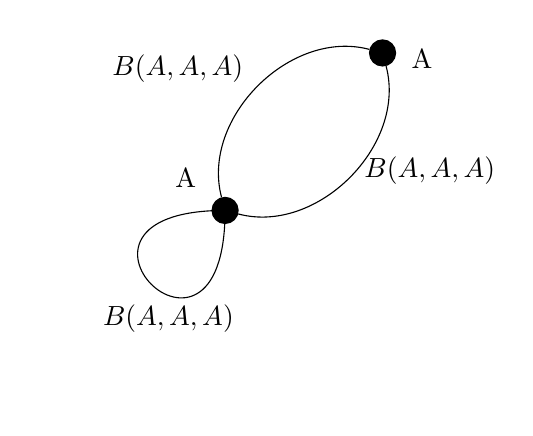
\begin{tikzpicture}
        \node[shape=circle, draw=black, fill, label={[xshift=-0.5cm, yshift=0.0cm]A}] (A) at (0,0) {} ;
        \node[shape=circle, draw=black, fill, label={[xshift=0.5cm, yshift=-0.5cm]A}] (B) at (2,2) {};
        \draw (A) edge[bend right=60] (B);
        \node (C) at (-0.6, 1.8) {$ B(A, A, A)$};
        \path [-] (A) edge[bend right=-60] (B);
        \node (C) at (2.6, 0.5) {$B(A, A, A)$};
        \draw[postaction={decorate}] 
        (0mm,0mm) 
          .. controls (-25mm,-0mm) and (-0mm,-25mm) ..
        (0mm,0mm)
          node[pos=0.6,below] {$ B(A, A, A)$};
    \end{tikzpicture}
    \caption{Example of a graph $G$ and sketch of the complex $A^{\otimes G}$. As graded vector spaces, $B = A\otimes T(\bar A[1])\otimes A$ where $T(\bar A[1]) = \bigoplus_{n\in \Z_{\geq 0}} \bar A[1]^{\otimes n}$. In this example, as graded vector spaces, $A^{\otimes G} = A^{\otimes 2} \otimes (T(\bar A[1]))^{\otimes 3}$, where each factor corresponds to a vertex or an edge. The differential is a sum of two differentials $d=d_0+d_1$ where $d_0$ is given by the differential of $A$ and $d_1$ is defined using the source and target maps of the graph and the product on $A$. }\label{fig:graph-model-example}
\end{figure}

Let $A$ be a DGCA. For any finite ordered set $S$, we can define the tensor product $A^{\otimes S} = \bigotimes_{s\in S} A$ and equip it with the usual tensor product chain complex and algebra structure. Given a map $f\colon S\to S'$ with $S = \{s_1,\dots, s_n\}$ and $S' = \{s'_1,\dots, s'_l\}$, we can construct a map $A^{\otimes S}\to A^{\otimes S'}$ using the algebra structure of $A$:
\begin{align*}
    a_{s_1}\otimes\dots\otimes a_{s_n}\mapsto (-1)^\epsilon \Prod_{f(s) =s'_1} a_s \otimes\dots \otimes \Prod_{f(s) =s'_l} a_s
\end{align*}
where $(-1)^\epsilon$ is the Koszul sign from reordering $a_{s_1}\otimes\dots\otimes a_{s_n}$ into the order on the right hand side. 

Let $A=\Omega^*(M)$ and $B = B(A, A, A)$. Consider the following maps
\begin{align*}
    \Phi\colon& (A^{\otimes 2})^{\otimes E}\to B^{\otimes E} \\
    \Psi\colon& (A^{\otimes 2})^{\otimes E} \to A^{\otimes V}\otimes A^{\otimes V}\to A^{\otimes V} 
\end{align*}
The map $\Phi$ is the product of the inclusions $A^{\otimes 2}\to B$, given simply by
$$a_{e_1}\otimes a'_{e_1}\otimes\dots\otimes a_{e_n}\otimes a'_{e_n} \mapsto (a_{e_1}\otimes a'_{e_1}) \otimes \dots\otimes (a_{e_n}\otimes a'_{e_n}).$$ 
The map $\Psi$ is induced by the map $s\coprod t\colon E\coprod E\to V\coprod V$ and the multiplication on $A$: it maps 
$$a_{e_1}\otimes a'_{e_1}\otimes\dots\otimes a_{e_n}\otimes a'_{e_n} \mapsto (-1)^\epsilon \Prod_{s(e) = v_1}a_e \Prod_{t(e) = v_1} a'_e \otimes \dots\otimes \Prod_{s(e) = v_n}a_e \Prod_{t(e) = v_n} a'_e$$
for $V = \{v_1,\dots, v_n\}$, where $\epsilon$ is the Koszul sign of permuting the factors $a_{e_1}, a'_{e_1}, \dots, a_{e_n}, a'_{e_n}$ into the sequence on the right hand side. 

We can relate $\phi^*, \psi^*$ to $\Phi, \Psi$ through the following diagram: 
\begin{center}
    \begin{tikzcd}
        B^{\otimes E} \dar["I^{\otimes E}"] & \lar["\Phi"] (A^{\otimes 2})^{\otimes E}\dar \rar["\Psi"] & A^{\otimes V} \dar[equal] \\
        \Omega^*(PM)^{\otimes E}\dar & \lar \Omega^*(M\times M)^{\otimes E} \dar\rar & \Omega^*(M)^{\otimes V}\dar \\
        \Omega^*(\Map(I, M)^{\times E}) \dar[equal] & \lar["\phi^*"]\dar[equal] \Omega^*(\Map(\{0, 1\}, M)^{\times E}) \rar["\psi^*"] & \Omega^*(\Map(\{pt\}, M)^{\times V})\dar[equal] \\
        \Omega^*(\Map(E\times I, M)) & \lar["\phi^*"] \Omega^*(\Map(E\times \{0, 1\}, M)) \rar["\psi^*"] & \Omega^*(\Map(V, M)) \\
    \end{tikzcd}
\end{center}

Thus $\Phi$ and $\Psi$ are models of $\phi$ and $\psi$:
\begin{lemma}\label{lem:graph-model-aid}
    There is a commutative diagram where each vertical map is a quasi-isomorphism:
    \begin{center}
        \begin{tikzcd}
            B^{\otimes E} \dar & \lar["\Phi"] (A^{\otimes 2})^{\otimes E}\dar \rar["\Psi"] & A^{\otimes V} \dar \\
            \Omega^*(\Map(E\times I, M)) & \lar["\phi^*"] \Omega^*(\Map(E\times \{0, 1\}, M)) \rar["\psi^*"] & \Omega^*(\Map(V, M)) \\
        \end{tikzcd}
    \end{center}
\end{lemma}

Recall that the tensor product $M\otimes_A N$ of two differential graded modules $M, N$ over a differential graded algebra $A$ is the quotient of the tensor product $M\otimes N$ by the differential ideal generated by $ma \otimes n - m\otimes an$ for homogeneous elements $m\in M, a\in A, n\in N$. 

Through the maps $\Phi, \Psi$, there is an $(A^{\otimes 2})^{\otimes E}$-module structure on $B^{\otimes E}$ and $A^{\otimes V}$. Our model of $\Omega^*(\Map(G, M))$ is defined as $A^{\otimes G} = B^{\otimes E}\otimes_{(A^{\otimes 2})^{\otimes E}} A^{\otimes V}$. One can show that $\Phi$ and $\Psi$ are maps of algebras and $A^{\otimes G}$ is the pushout in the category of differential graded commutative algebras. Thus $A^{\otimes G}$ is defined as the pushout of the model and we have an algebraic analogue of diagram \ref{diag:mapping-space-pullback}:

\begin{center}\label{diag:mapping-space-pullback-algebraic}
    \begin{tikzcd}
        (A^{\otimes 2})^{\otimes E} \dar["\Phi"] \rar["\Psi"] & A^{\otimes V} \dar \\
        B^{\otimes E} \rar & A^{\otimes G}
    \end{tikzcd}
\end{center}


\begin{construction}
    For a finite ordered graph $G$ and a manifold $M$, the \emph{iterated integral map}\index{iterated integral map!for graph mapping spaces} for $\Map(G, M)$ is the composition
    \begin{align*}
        I_G\colon A^ {\otimes G}\to\Omega^*(\Map(E\times I, M))\otimes_{\Omega^*(\Map(E\times\{0,1\}, M))} \Omega^*(\Map(V, M)) \to \Omega^*(\Map(G, M))
    \end{align*}
\end{construction}

\begin{remark}
    We can explicitly compute the map $$I_G\colon A^{\otimes G}\to \Omega^*(\Map(G, M)).$$ As graded vector spaces, $A^{\otimes G}$ is a direct sum of $\bigotimes_{e\in E} A[1]^{k_e}\oplus A^{\otimes V}$ over all $k_e\geq 0$ for $e\in E$: the outer $A$ factors of the bar construction are identified with the $A$ factors of the vertices by taking the tensor product relative to $(A^{\otimes 2})^{\otimes E}$. Write $s=\sum_{e\in E} k_e$. On each direct summand, $I_G$ is given by 
\begin{align*}
    \bigotimes_{e\in E} A[1]^{\otimes k_e} \otimes A^{\otimes V} \to \Omega^{*+s}\left(M^{s+|V|}\right)\xto{ev^*} \Omega^{*+s}\left(\Map(G, M) \times \Prod_{e\in E} \Delta^{k_e}\right) \xto{\int} \Omega^*(\Map(G, M))
\end{align*}
where the evaluation map $$ev=ev_{\{k_e\}}\colon \Map(G, M)\times \Prod_{e\in E} \Delta^{k_e} \to  M^{s+|V|}$$ evaluates each element of the mapping space at the times in $\Delta^{k_e}$ along the edge $e$ and at each vertex $v$. 

For example, if $G=\ocircle_1=S^1$ is the circle with one vertex and one edge, then $ev_n\colon LM\times \Delta^n\to M^n\times M$ is given by mapping $t_1,\dots, t_n, \gamma\mapsto \gamma(t_1),\dots,\gamma(t_n), \gamma(0)$.
\end{remark}

To apply \cref{thm:pullback-pushout} we need to add the assumption that $M$ is of finite type. Here a manifold is called of finite type if its cohomology is finite dimensional in each degree. 

\begin{theorem}\label{thm:graph-mapping-space}
    Let $M$ be a simply connected manifold and of finite type. Then the iterated integral map 
    $$I_G\colon A^{\otimes G} \to \Omega^*(\Map(G, M)).$$
    is a quasi-isomorphism, hence $A^ {\otimes G}$ is a model of $\Map(G, M)$.

    Moreover, for a morphism of graphs $G\to G'$, there is a commutative diagram
    \begin{center}
    \begin{tikzcd}
        A^{\otimes G} \dar \rar["I_G"] & \Omega^*(\Map(G, M)) \dar \\
        A^{G'}\rar["I_{G'}"] & \Omega^*(\Map(G', M))
    \end{tikzcd}
    \end{center}
\end{theorem}
\begin{proof}
    We can apply the pullback-pushout theorem \ref{thm:pullback-pushout} to the pullback diagram of $\Map(G, M)$
    \begin{center}
        \begin{tikzcd}
            \Map(E\times \{0, 1\}, M) & \lar["\phi"] \Map(V, M)  \\
            \Map(E\times I, M) \uar["\psi"] & \lar \Map(G, M) \uar
        \end{tikzcd}
    \end{center}
    All spaces here are connected and simply connected since $M$ is. The map $\Map(E\times I, M)\to\Map(\{0,1\}\times E, M)$ is a Serre fibration (it is a product of the evaluation maps $PM\to M\times M$) hence the diagram is a homotopy pullback diagram. 

    Consider the following commutative diagram:
    \begin{center}
        \[
        \begin{tikzcd}[column sep = 2em, center picture]
            \Omega^*(M^{I\times E})\otimes^L_{\Omega^*(M^{\{0, 1\}\times E})} \Omega^*(M^V) \rar& \Omega^*(M^{I\times E})\otimes_{\Omega^*(M^{\{0, 1\}\times E})} \Omega^*(M^V) \rar & \Omega^*(M^G) \\
            B^{\otimes E}\otimes^L_{(A^{\otimes 2})^{\otimes E}} A^{\otimes V} \rar["\quiso"]\uar["\quiso"]& B^{\otimes E}\otimes_{(A^{\otimes 2})^{\otimes E}} A^{\otimes V} = A^{\otimes G}\uar
        \end{tikzcd}
        \]
    \end{center}
    The vertical maps are induced by the diagram in \cref{lem:graph-model-aid}.
    The map $(A^{\otimes 2})^{\otimes E} \to B^{\otimes E}$ is a tensor product of the maps $A^{\otimes 2}\to B$, hence a cofibration over $(A^{\otimes 2})^{\otimes E}$, see \cref{lem:bar-cofibrant}. Hence the lower map is a quasi-isomorphism by \cref{thm:bar-resolution-sullivan}. The left vertical map is a quasi-isomorphism because it is a quasi-isomorphism on each of the factors, see \cref{thm:bar-quiso}. Finally, the composition of the top horizontal maps is a quasi-isomorphism by the pullback-pushout lemma \ref{thm:pullback-pushout}, using \cref{assumption}. We conclude that the map $A^{\otimes G} \to \Omega^*(\Map(G, M))$ is a quasi-isomorphism. 
\end{proof}


We can now easily give models for common spaces and maps in string topology. Let $\ocircle_1$ be the graph with one vertex and one edge, thus $LM = \Map(\ocircle_1, M)$. Further let $8$ be the graph with one vertex and two edges, so $LM\times_M LM = \Map(8, M)$. Let $\ocircle_2$ be the circle graph with two points and let $\ocircle_1\coprod \ocircle_1$ be the coproduct of graphs (disjoint union) of two copies of $\ocircle_1$.
\begin{corollary}\label{lem:model-quasi-iso-examples}
    The following maps are quasi-isomorphisms if $M$ is simply connected and of finite type.
    \begin{align*}
        B\otimes_{A^{\otimes 2}} A \xto{I_{\ocircle_1}} \Omega^*(LM)
    \end{align*}
    \begin{align*}
        (B\otimes B)\otimes_{A^{\otimes 2}\otimes A^{\otimes 2}} A^{\otimes 2} \xto{I_{\ocircle_2}}\Omega^*(Map(\ocircle_2, M))
    \end{align*}
    \begin{align*}
        (B\otimes B)\otimes_{A^{\otimes 2}\otimes A^{\otimes 2}} A \xto{I_{8}} \Omega^*(Map(8, M))
    \end{align*}
    \begin{align*}
        (B\otimes_{A^{\otimes 2}}A) \otimes (B\otimes_{A^{\otimes 2}} A) \xto{I_{\ocircle_1\coprod\ocircle_1}} \Omega^*(LM\times LM)
    \end{align*}
    \begin{align*}
        B\otimes_A B\to \Omega^*(PM\times_M PM)
    \end{align*}

    The following diagram commutes:
    \begin{center}
    \begin{tikzcd}
        (B\otimes B)\otimes_{A^{\otimes 4}} A \rar["I_8"] & \Omega^*(\Map(8)) \\
        (B\otimes_{A^{\otimes 2}}A) \otimes (B\otimes_{A^{\otimes 2}} A)\uar \rar["\ocircle_1\coprod \ocircle_1"] & \Omega^*(LM\times LM) \uar
    \end{tikzcd}
    \end{center}
\end{corollary}
The diagram follows from the naturality of $I$ with respect to the map $\ocircle_1\coprod \ocircle_1\to 8$.


\subsection{Model for the concatenation and splitting map}\label{subsec:model-concatenation} 
Concatenating and splitting up paths is not modeled by the theory of the previous subsection. 

The \emph{concatenation of paths} is defined as the map 
\begin{align*}
    c\colon PM\times_mPM&\to PM \\
    c(\gamma_1, \gamma_2)(t) &= \begin{cases}\gamma_1(\frac 12 t)&\text{if}\ t\leq\frac 12 \\ \gamma_2(\frac 12 t + \frac 12) & \text{if}\ t\geq \frac 12 \end{cases}
\end{align*}
This induces a concatenation of loops $c\colon LM\times_MLM \to LM$.
We model the concatenation of paths by the \emph{deconcatenation coproduct} on $B$
\begin{align*}
    \bar c\colon B&\to B\otimes_A B \\
    a\otimes a_1 \otimes \dots \otimes a_n \otimes a'&\mapsto \sum_{k+l=n} a\otimes a_1 \otimes \dots \otimes a_k \otimes  1 \otimes a_{k+1} \otimes \dots \otimes a_{k+l} \otimes  a'
\end{align*}
The following lemma shows that $\bar c$ models the concatenation of paths $c$ on cohomology and $\bar c\otimes\id\colon B\otimes_{A^{\otimes 2}}\to (B\otimes B)\otimes_{A^{\otimes 2}\otimes A^{\otimes 2}} A$ models the concatenation of loops. 
\begin{lemma}\label{lem:model-concatenation}
    Let $c\colon PM\times_M PM\to PM$ be the concatenation of paths. The following diagrams commute:
    \begin{equation}\label{diag:concatenation}
        \begin{tikzcd}
            B \rar \dar["\bar c"] & \Omega^*(PM) \dar["c^*"] \\
            B \otimes_A B \rar & \Omega^*(PM\times_M PM)
        \end{tikzcd}
    \end{equation}
    \qquad
    \begin{equation}\label{diag:concatenation-2}
    \begin{tikzcd}
        (B\otimes B)\otimes_{A^{\otimes 2}\otimes A^{\otimes 2}} A\rar["I_{8}"] &\Omega^*(LM\times_M LM) \\
        B\otimes_{A^{\otimes 2}}A \uar["\bar c"]\rar["I_{\ocircle_1}"] & \Omega^*(LM) \uar["c^*"]
    \end{tikzcd}
    \end{equation}
\end{lemma}
\begin{proof}
    This is stated in \cite{naef2019string} without proof. We give a detailed proof here. 
    \begin{enumerate}
        \item For diagram \ref{diag:concatenation}: let $k+l=n$, consider the maps
        \begin{align*}
            d_{k,l}\colon \Delta^k\times\Delta^l&\to \Delta^n\\
            (t_1, \dots, t_k), (t_{k+1}, \dots, t_{k+l}) &\mapsto \left(\frac 12 t_1, \dots, \frac 12 t_k, \frac 12 + \frac 12 t_{k+1}, \dots, \frac 12 + \frac 12 t_{k+l}\right)
        \end{align*}
        so that the images of the $d_{k,l}$ cover $\Delta^n$ and are disjoint except at the boundary. Consider the following diagram with $k+l=n$. 

% \begin{figure}\label{fig:path_models_1}
    \[
    \begin{tikzcd}[font=\footnotesize, column sep = 2em, center picture]
        A^{\otimes n+2}[n] \rar\dar & \Omega^{*+n}(M^{n+2}) \rar["ev^*"]\dar & \Omega^{*+n}(PM\times \Delta^n) \rar["\int_{\Delta^n}"]\dar["(d_{k,l}\times c)^*"] & \Omega^*(PM) \dar["c^*"] \\
        A^{\otimes k+l+3}[n] \rar & \Omega^{*+n}(M^{k+2}\times_M M^{l+2}) \rar["ev_{k,l}"] & \Omega^{*+n}(PM\times_M PM\times \Delta^k\times\Delta^l) \rar["\int_{\Delta^k\times\Delta^l}"] & \Omega^*(PM\times_M PM)\\
        %A^{\otimes k+2}[k]\otimes_{A} A^{\otimes l+2}[l] \rar\uar["\iso"] & \Omega^{*+k}(M^{k+2})\otimes_{A} \Omega^{*+l}(M^{l+2}) \uar\rar & \Omega^{*+k}(PM\times\Delta^k)\otimes_{A} \Omega^{*+l}(PM\times\Delta^l) \rar["\int_{\Delta^k}\otimes\int_{\Delta^l}"]\uar & \Omega^*(PM)\otimes_{A} \Omega^*(PM) \uar
    \end{tikzcd}
    \]
% \end{figure}

All squares commute except for the right, which commutes only after summing over all $k, l$ with $k+l=n$: 

\begin{align*}
    c^*\int_{\Delta^n}\omega &= c^*\sum_{k+l=n} \int_{\mathrm{im} (d_{k,l})} \omega \\
    &= \sum_{k+l=n} \int_{\Delta^k\times\Delta^l} (c\times d_{k,l})^*\omega
\end{align*}

The left hand side is the upper path of the square, the right hand side is the lower path of the square, up to commuting the factors. This concludes the proof for diagram \ref{diag:concatenation}.

    \item For diagram \ref{diag:concatenation-2}: By applying the functor $\blank \otimes_{A^{\otimes 2}} A$ to diagram \ref{diag:concatenation}, we obtain the diagram
    \begin{center}
        \begin{tikzcd}
            (B\otimes_A B)\otimes_{A^{\otimes 2}} A\rar["I_{\ocircle_2}"] &\Omega^*(\ocircle_2) \\
            B\otimes_{A^{\otimes 2}}A \uar\rar["I_{\ocircle_1}"] & \Omega^*(LM) \uar
        \end{tikzcd}
    \end{center}
    The inclusion $\Map(\ocircle_2, M)\to LM\times_M LM$ is modeled by the diagram
    \begin{center}
        \begin{tikzcd}
            (B\otimes_A B)\otimes_{A^3} A\rar &\Omega^*(LM\times_M LM) \\
            (B\otimes_A B)\otimes_{A^{\otimes 2}} A\rar \uar &\Omega^*(\ocircle_2) \uar\\
        \end{tikzcd}
    \end{center}
    as in \ref{thm:graph-mapping-space}, via the map of graphs $\ocircle_2\to 8$ mapping the two points to the pinch point of the figure $8$. Combining the two diagrams, we obtain the diagram as claimed.
\end{enumerate}
\end{proof}

Recall that the splitting of paths map is defined as
\begin{align*} 
    s\colon I\times PM &\to PM\times_M PM\\
    s(t, \gamma)&=\left(r(\gamma|_{[0, t]}) , r(\gamma|_{[t, 1]})\right)
\end{align*}
where $r$ is the reparametrization map which maps a path defined on any interval to a path on the interval $[0,1]$. We denote the induced map $I\times LM\to \Map(\ocircle_2, M)$ by $s$ as well.

% \begin{remark}Recall that in order to even define $\Omega^*(LM)$, we have to use the smooth loop space. The concatenation of smooth loops $LM\times_M LM\to LM$ will generally not yield smooth loops. To fix this, we replace the smooth loop space with the subspace of smooth loops which are constant near $0\in S^1=\R/\Z$. One can show that this subspace is homotopy equivalent to the original smooth loop space, using a homotopy between the identity of $S^1$ and a map $S^1\to S^1$ which is constant near $0$. Similarly we replace $LM\times_M LM$ by the subspace of maps $S^1\vee S^1\to M$ which are constant near $0$ and similar replacements apply to $LM$. 
% \end{remark}

We introduce a model of the interval $\mathcal I = \R (1-t) \oplus \R t \oplus \R dt\subset \Omega^*(I)$, the space of Whitney forms on the interval. There is a projection 
\begin{align*}
    \Omega^*(I) &\to \mathcal I\\
    f&\mapsto f(0)(1-t) + f(1) t + \left(\int_I f\right) dt
\end{align*}
which is a quasi-isomorphism with quasi-inverse given by the inclusion $$\iota_{\mathcal I}\colon \mathcal I \subset \Omega^*(I).$$ 

Recall from \cref{thm:path-models-0} that $\alpha\colon B\to A$ is given the direct summands of $B$ by the product for $n=0$ and $0$ for $n>0$.

We model the splitting map $s$ by the map 
\begin{align*}
    \bar s \colon B\otimes_A B&\to \mathcal I\otimes B \\
    a_1 \otimes \gamma_1 \otimes a_2 \otimes \gamma_2 \otimes a_3 &\mapsto  (1-t) \otimes \alpha (a_1 \otimes \gamma_1 \otimes a_2)1_A \otimes \gamma_2 \otimes a_3 \\
    &\quad+ t\otimes a_1 \otimes \gamma_1 \otimes 1_A \alpha (a_2 \otimes \gamma_2 \otimes a_3)  \\
    &\quad +  (-1) ^{\abs{a_1\gamma_1a_2}} dt\otimes a_1 \otimes (\gamma_1\otimes a_2\otimes \gamma_2) \otimes a_3
\end{align*}
for $a_i\in A, \gamma_1\in A[1]^{\otimes k}, \gamma_2\in A[1]^{\otimes l}$.

The following is a slight reformulation of \cite{naef2019string}{Prop. 4.2}.
\begin{theorem}\label{thm:model-splitting}
    The following diagrams commute in the derived category of chain complexes $D(Ch_\R)$:

    \begin{tikzcd}
        \mathcal I \otimes B \rar["\iota_{\mathcal I} \times I"] & \Omega^*(I\times PM) \\
        B\otimes_A B \rar["I"] \uar["\bar s"] &\Omega^*(PM\times_M PM) \uar["s^*"]
    \end{tikzcd}
    \qquad
    \begin{tikzcd}
        \mathcal I \otimes (B\otimes_{A^{\otimes 2}} A) \rar["\iota_{\mathcal I}\times I"] & \Omega^*(I\times LM) \\
        (B\otimes_A B)\otimes_{A^{\otimes 2}} A \rar["I"] \uar & \Omega^*(\Map(\ocircle_2, M))\uar["s^*"]
    \end{tikzcd}
\end{theorem}
All the horizontal maps are quasi-isomorphisms from \cref{thm:graph-mapping-space}.

For spaces $X, Y$ and forms $\omega_1\in\Omega^*(X), \omega_2\in\Omega^*(Y)$, we write $\omega_1\times\omega_2 = p_1^*\omega_1 \wedge p_2\omega_2\in\Omega^*(X\times Y)$, where $p_1\colon X\times Y\to X$ and $p_2\colon X\times Y\to Y$ are the projections.

\begin{proof}
    %This is stated in \cite{naef2019string} without proof. We give a detailed proof here. 
    The second diagram follows from the first diagram, by a similar argument as in the proof of \cref{lem:model-concatenation}. Thus we only consider the first diagram.

    We factor $s^*$ through $\mathcal I\otimes \Omega^*(PM)$. There is a quasi-isomorphism $\mathcal I\otimes\Omega^*(PM)\to \Omega^*(I\times PM)$ given by $\iota_{\mathcal I}\times\id$ with quasi-inverse and left inverse given by 
    \begin{align*}
        k\colon\Omega^*(I\times PM) &\to \mathcal I \otimes \Omega^*(PM) \\
        \omega & \mapsto (1-t)\omega|_{t=0} + t\ \omega|_{t=1} + dt \int_I \omega
    \end{align*}
    where $\omega|_{t=0,1}$ is the image of $\omega$ under the pullback of the inclusion $PM\to I\times PM$ at $t=0$ resp.\ $t=1$.

    Denote by $\epsilon_{0}$ resp.\ $\epsilon_1\colon PM\to PM\times_M PM$ the maps $\gamma\mapsto \mathrm{const}(\gamma(0))\times \gamma$ resp.\ $\gamma\mapsto \gamma\times \mathrm{const}(\gamma(1))$. The composition $\hat s = k\comp s^*$ is
    \begin{align*}
        \hat s\colon \Omega^*(PM\times_M PM)\to \mathcal I\otimes\Omega^*(PM)\\
        \omega \mapsto (1-t)\ \epsilon_0^*(\omega) + t\ \epsilon_1^*(\omega) + dt \int_I s^*\omega
    \end{align*}

    In $D(Ch_{\R})$, the maps $k$ and $\iota_{\mathcal I}\times \id$ are inverses and hence $(\iota_{\mathcal I}\times \id)\comp \hat s = s^*$. Hence in $D(Ch_{\R})$, the map $s^*$ is  equal to the map
    \begin{align*}
        \hat s\colon \Omega^*(PM\times_M PM)\to \Omega^*(I\times PM)\\
        \omega \mapsto (1-t)\ \epsilon_0^*(\omega) + t\ \epsilon_1^*(\omega) + dt \int_I s^*\omega
    \end{align*}

    Since the constant map $M\to PM$ is modeled by $\alpha$ from \cref{thm:path-models-0}, the maps $\epsilon_i$ are modeled by $\alpha\otimes\id$ resp.\ $\id\otimes\alpha\colon B\otimes_A B\to B$.
    
    It remains to give an algebraic model of the map $\omega\mapsto \int_I s^*\omega$. Let $r\colon \Delta^k\times\Delta^l\times I\to \Delta^{n+1}$, mapping $(s_1,\dots, s_k), (t_1,\dots, t_k), t\mapsto (ts_1, \dots, ts_k, t+(1-t)t_1, \dots, t+(1-t)t_l)$ and similarly $r'\colon \Delta^k\times I\times\Delta^l\to \Delta^{n+1}$, equal to $r$ up to swapping the factors. We consider the following diagram in the derived category, where $k+l=n$:
    \[
    \begin{tikzcd}[center picture]
        \Omega^{*}(PM\times_M PM)\dar["s^*"] & \lar["\int_{\Delta^k\times\Delta^l}"] \Omega^{*+k+l}(PM\times_M PM\times \Delta^k\times \Delta^l )\dar["(\id\times s)^*"] & \lar["ev_{k,l}"]  \Omega^{*+k+l}(M^{1+k+1+l+1})\dar[equal] \\
        \Omega^{*}(PM\times I) \dar["\int_I"] &\lar["\int_{\Delta^k\times\Delta^l}"] \Omega^{*+k+l}(PM\times I\times \Delta^k\times\Delta^l) \dar[equal] & \lar["(ev\comp (\id\times r)^*"] \Omega^{*+k+l}(M^{1+k+1+l+1}) \dar[equal] \\
        \Omega^{*-1}(PM) \dar["\pm\id"] & \lar["\int_{\Delta^k\times\Delta^l\times I}"] \dar \Omega^{*+k+l}(PM\times I\times \Delta^k\times\Delta^l) &\lar["(ev\comp (\id\times r)^*"]\dar \Omega^{*+k+l}(M^{1+k+1+l+1}) \\
        \Omega^{*-1}(PM) \dar[equal] & \lar["\int_{\Delta^k\times I\times \Delta^l}"] \dar["(\id\times r')^!"] \Omega^{*+k+l}(PM\times \Delta^k\times I\times\Delta^l) &\lar["(ev\comp (\id\times r')^*"]\dar["\id"] \Omega^{*+k+l}(M^{1+k+1+l+1}) \\
        \Omega^{*-1}(PM) & \lar["\int_{\Delta^{n+1}}"] \Omega^{*+n}(PM \times \Delta^{n+1}) &\lar["ev_{n+1}^*"] \Omega^{*+n}(M\times M^{n+1}\times M)
    \end{tikzcd}
    \]
   
    Everything except for the lower two squares commutes on the chain level. We cannot construct the umkehr map $(\id\times r')^!\colon\Omega^{*+k+l}(PM\times \Delta^k\times I\times\Delta^l)\to \Omega^{*+n}(PM\times \Delta^{n+1})$ via a fiber integral on the chain level, as we have done for other umkehr maps so far: $r'$ has finite fiber almost everywhere, but we have restricted ourselves to de Rham forms that are smooth and defined everywhere. We work in the derived category instead and pass to the singular cochain complex. 
    
    Let $p_{\Delta^k\times I\times\Delta^l}\colon M\times\Delta^k\times\Delta^l\times I \to M$ and $p_{\Delta^{n+1}}\colon M\times \Delta^{n+1}\to M$ be the projections. We replace the lower two squares with the quasi-isomorphic diagram
    \begin{center}
    \begin{tikzcd}
        C^{*-1}(M) \dar[equal] & \lar["p_{\Delta^k\times I\times\Delta^l}^!"] C^{*+k+l}(M\times \Delta^k\times I\times\Delta^l) \dar["(\id\times r)^!"] & \lar["(\Delta\comp(\id\times r))^*"] C^{*+k+l}(M^{1+k+1+l+1}) \dar["\pm\id"]\\
        C^{*-1}(M) & \lar["p_{\Delta^{n+1}}^!"] C^{*+n}(M\times \Delta^{n+1}) &\lar["\Delta^*"] C^{*+n}(M^{1+(n+1)+1})
    \end{tikzcd}
    \end{center}
    The umkehr map in the center can be constructed in $D(Ch_\R)$, because both spaces satisfy Poincaré duality relative to their boundary, compare \cref{subsec:umkehr_maps_via_pd}. 
    We then construct the map $\Omega^{*+k+l}(\Delta^k\times I\times \Delta^l\times PM)\to \Omega^{*+n}(\Delta^{n+1}\times PM)$ in $D(Ch(\R))$ as the map in the center, taken through the isomorphisms between the diagrams. Since umkehr maps compose, the left square commutes. To compute the umkehr map $r'^!$, since the map $r'\colon (\Delta^k\times I\times \Delta^l, \partial \Delta^k\times I\times \Delta^l)\to (\Delta^{n+1}, \Delta^{n+1})$ preserves the orientation, the fundamental class is preserved by $r_*$. So $r^!$ maps $1$ to $1$ and since both spaces are contractible, this determines $r^!$ uniquely in the derived category. On the other hand, $r^*$ maps $1$ to $1$, hence the composition is $r'^! r'^* = \id$. In fact, $(r'\times \id)^!(\id\times r')^* = \id$. This shows that the right diagram commutes. 

    Thus we have shown that the following commutes in $D(Ch(k))$: 

    \begin{center}
        \begin{tikzcd}
        \Omega^*(PM\times_M PM)\dar["\int_I s^*\omega"] &\lar B\otimes_A B \dar \\
        \Omega^{*-1}(PM) & \lar B[-1]
    \end{tikzcd}
    \end{center}
    where the right vertical map is $a_1(\gamma_1)a_2(\gamma_2)a_3 \mapsto (-1)^{\abs{a_1\gamma_1a_2}} a_1(\gamma_1|a_2|\gamma_2)a_3$. Hence we are done.
    % \[
    % \begin{tikzcd}[center picture]
    %     \Omega^*(PM\times_M PM) \dar & \lar \Omega^{*+k+l}((\Delta^k\times PM) \times_M(\Delta^k\times PM)) \dar & \lar \Omega^{*+k+l}(M^{1+k+1+l+1}) \dar \\
    %     \Omega^{*}(PM\times_M PM)\dar & \lar["\int_{\Delta^k\times\Delta^l}"] \Omega^{*+k+l}(\Delta^k\times \Delta^l \times PM\times_M PM)\dar & \lar  \Omega^{*+k+l}(M^{1+k+1+l+1})\dar \\
    %     \Omega^{*}(I\times PM) \dar["\id"] &\lar["\int_{\Delta^k\times\Delta^l}"] \Omega^{*+k+l}(\Delta^k\times\Delta^l\times I\times PM) \dar["\wedge dt"] & \lar \Omega^{*+k+l}(M^{1+k+1+l+1}) \dar["\wedge dt"] \\
    %     \Omega^{*}(I\times PM) \dar["\id"] & \lar["\int_{\Delta^k\times\Delta^l\times I}"] \dar \Omega^{*+k+l+1}(\Delta^{k}\times\Delta^l\times I\times I \times PM) &\lar\dar \Omega^{*+k+l+1}(I\times M^{1+k+1+l+1}) \\
    %     \Omega^{*}(I\times PM) & \lar["\int_{\Delta^{n+1}}"] \Omega^{*+n+1}(\Delta^{n+1} \times I\times PM) &\lar \Omega^{*+n+1}(I\times M\times M^{n+1}\times M)
    % \end{tikzcd}
    % \]
    % \begin{tikzcd}
    %     \Omega^{*+1}(PM\times_M PM) \dar & \lar\dar B\otimes_A B\\
    %     \Omega^{*+1}(I\times PM) \dar & \lar\dar  \mathcal I \otimes B \\
    %     \Omega^*(PM) & \lar B
    % \end{tikzcd}
\end{proof}

\begin{remark}
    In \cite{naef2019string} it is also stated that the wedge product on $\Omega^*(PM)$ corresponds to the shuffle product $\shuffle$ (see \cref{def:shuffle-product}) on $B(\Omega^*(M), \Omega^*(M), \Omega^*(M))$:
    \begin{center}
    \begin{tikzcd}
        B\otimes B\dar["\shuffle"] \rar["I\otimes I"]&\Omega^*(PM)\otimes\Omega^*(PM) \dar["\wedge"]\\
        B \rar["I"] & \Omega^*(PM)
    \end{tikzcd}
    \end{center}

    No proof is given in \cite{naef2019string}. We only give a sketch of a proof since we will not use this statement later. The wedge product of the fiber integrals over $\Delta^k$ and $\Delta^l$ in $I(a(a_1|\dots|a_k)a') \wedge I(b(a_{k+1}|\dots|a_{k+l})b')$ can be rewritten as a fiber integral over $\Delta^k\times\Delta^l$ of a single differential form. By an Eilenberg-Zilber argument, one can decompose $\Delta^{k}\times\Delta^k$ into copies of $\Delta^{k+l}$, using shuffle permutations and the degeneracy maps $\Delta^{k+l}\to \Delta^k, \Delta^{k+l}\to \Delta^l$. So the fiber integral is a sum of fiber integrals of certain classes over $\Delta^{k+l}$. With some work, one can represent this again as a sum of iterated integrals.
\end{remark}





\section{Algebraic Models of String Topology Operations}\label{sec:loop-models}
As an application of the previous subsection, we are able to describe maps involved in the construction of the string topology operations, such as the inclusion $LM\times_M LM\to LM\times LM$ and the composition $LM\times_M LM\to LM$. In \cref{subsec:loop-product-model} we give a model of the loop product using Hochschild homology and show that the iterated integral map intertwines this with the loop product in the derived category. We also show that the different constructions of the loop product via configuration spaces from \cref{subsec:loop-product} and via tubular neighborhoods and the Thom isomorphism from \cref{subsec:loop-product-classical} yield the same maps on cohomology. In \cref{subsec:poincare-algebra} we explain how one can obtain a chain level model of the loop coproduct. In \cref{subsec:co-bv-alg} we show that the iterated integral map from the Hochschild complex into $\Omega^*(LM)$ preserves the co-BV operator as a map of derived chain complexes. In particular this gives a proof that the Chas-Sullivan operations satisfy the co-BV algebra relations  on cohomology in the simply connected case. 

\subsection{Loop Product Model (Cohomology Coproduct)}\label{subsec:loop-product-model}
To give a model of the Loop product we need to model the intersection map $i^!\colon H^*(LM\times LM) \from H^{*-n}(LM\times_M LM)$. In \cref{constr:loop-intersection-via-configuration} we constructed this as the following zigzag in $D(Ch)$:
\begin{center}
    \begin{tikzcd}[column sep = 1em, center picture, font=\small]
        \Omega^*(LM\times LM) &\lar \cone\left(\Omega^*(LM\times LM)\to \Omega^*(LM\times LM|_{\cConf_M(2)})\right) \dar["\quiso"] & \\ 
        & \cone\left(\Omega^*(LM\times LM|_M)\to \Omega^*(LM\times LM|_{UTM})\right) & \lar \Omega^{*-n}(LM\times LM|_M)[-n]
    \end{tikzcd}
\end{center}
Here $\cone$ denotes the mapping cone. Using the pullback-pushout lemma \ref{thm:pullback-pushout} we can rewrite this, using the derived relative tensor product $M\otimes^L_{A^{\otimes 2}}N$ over the DGCA $A^{\otimes 2}$. This can be constructed as the bar construction $M\otimes^L_A N = B(M, A, N)$, compare \cref{subsec:bar_construction}. Let $A=\Omega^*(M)$ and $D = \Omega^*(LM)$, then the zigzag above can be rewritten as: 
\begin{center}
    \begin{tikzcd}[center picture]
        D^{\otimes 2} &\lar \cone\left(D^{\otimes 2}\to D^{\otimes 2}\otimes^L_{A^{\otimes 2}}\Omega^*(\cConf_M(2))\right) \dar["\quiso"] &
        \\ & \cone\left(D^{\otimes 2}\otimes^L_{A^{\otimes 2}} A \to D^{\otimes 2} \otimes^L_{A^{\otimes 2}} \Omega^*(UTM) \right) & \lar D^{\otimes 2}\otimes^L_{A^{\otimes 2}} A[-n] 
    \end{tikzcd}
\end{center}
which comes with a quasi-isomorphism to the original zigzag. 


% Assume we have a model for the inclusion $UTM = \partial \cConf_M(2)\to \cConf_M(2)$, hence a diagram
% \begin{center}
%     \begin{tikzcd}
%         C\rar\dar["\quiso"] & U \dar["\quiso"] \\
%         \Omega^*(\cConf_M(2)) \rar & \Omega^*(UTM)
%     \end{tikzcd}
% \end{center} 
% Using the models from the previous subsection, we can rewrite the above zigzag again:
% \begin{center}
%     \begin{tikzcd}[font=\footnotesize, column sep = 1em, center picture]
%         B\otimes_{A^{\otimes 2}} A\otimes B\otimes_{A^{\otimes 2}} A & \lar \cone\left(B\otimes_{A^{\otimes 2}} A\otimes B\otimes_{A^{\otimes 2}} A \to (B\otimes B) \otimes_{A^{\otimes 2}\otimes A^{\otimes 2}} C\right) \dar["\quiso"] && \\
%         &\cone\left(B\otimes_{A^{\otimes 2}} B \otimes_{A^{\otimes 2}} A \to B\otimes_{A^{\otimes 2}} B\otimes_{A^{\otimes 2}} U\right) & \lar B\otimes_{A^4} B[-n] & \lar B\otimes_{A^{\otimes 2}} A[-n]
%     \end{tikzcd}
% \end{center}
The new zigzag can be obtained from the following much simpler zigzag of $A$-bimodules by tensoring with $D^{\otimes 2}$ over $A^{\otimes 2}$:
\begin{center}
    \begin{tikzcd}
        A\otimes A & \lar \cone(A\otimes A \to \Omega^*(\cConf_M(2))) \dar["\quiso"]& \\
        & \cone(A \to \Omega^*(UTM)) & \lar A[-n]
    \end{tikzcd}
\end{center}

and this is the intersection map $\Delta^!\colon\Omega^*(M\times M)\from \Omega^{*-n}(M)$ as constructed in \ref{subsec:intersection-in-M-via-conf}. Thus we conclude the following lemma:

\begin{lemma}
    The following diagram commutes in $D(Ch)$:
    \begin{center}
    \begin{tikzcd}
        \Omega^*(LM\times LM) & \lar["i^!"] \Omega^{*}(LM\times_M LM)[-n]  \\
        \uar["\quiso"] \Omega^*(LM)\otimes \Omega^*(LM) \otimes^L_{A^{\otimes 2}} A^{\otimes 2} & \uar["\quiso"]\lar["\id\otimes\Delta^!"] \Omega^*(LM)\otimes \Omega^*(LM) \otimes^L_{A^{\otimes 2}} A[-n]
    \end{tikzcd}
    \end{center}
    The map $\Delta^!\colon \Omega^*(M)[-n]\to\Omega^*(M)\otimes \Omega^*(M)$ is the intersection coproduct of $M$, see \cref{subsec:intersection-in-M-via-conf}.
\end{lemma}
With a similar analysis of the classical construction of the loop product from \ref{constr:loop-product-classical}, one can show the same lemma for the intersection map there. Thus we can show the following:

\begin{corollary}\label{thm:loop-products-identity}
    Let $M$ be a closed oriented, simply connected manifold. Let $A = \Omega^*(M)$.

    The two constructions of the derived intersection map $i^!\colon\Omega^*(LM\times LM) \from \Omega^{*}(LM\times_M LM)[-n]$ from \cref{subsec:loop-product-classical} and \cref{constr:loop-intersection-via-configuration} are equal as maps in $D(Ch(\R))$. In particular they are the same on cohomology.
\end{corollary}

\begin{theorem}\label{thm:loop-product-derived}
    Let $M$ be a closed oriented, simply connected manifold. Let $A = \Omega^*(M)$ and $B=B(A, A, A)$ the bar construction of $A$.
    The following diagram in $D(Ch)$ commutes:
    \begin{center}
    \begin{tikzcd}
        \Omega^*(LM)\otimes\Omega^*(LM) & \lar["i^!"] \Omega^*(LM\times_M LM)[-n] & \lar["c"] \Omega^*(LM)[-n] \\
        B\otimes_{A^{\otimes 2}} A\otimes B\otimes_{A^{\otimes 2}} A \uar["\quiso"] & \lar["\id\otimes\Delta^!"] B^{\otimes 2}\otimes_{A^{\otimes 4}} A\uar["\quiso"] & B\otimes_{A^{\otimes 2}} A \lar["\bar c"]\uar["\quiso"]
    \end{tikzcd}
    \end{center}
    The upper horizontal composition is the loop product (cohomology coproduct). The vertical quasi-isomorphisms are iterated integral type maps (see \cref{thm:graph-mapping-space}). The lower horizontal composition is induced by the intersection coproduct on $A$ and the deconcatenation coproduct on $B\to B\otimes_A B$ (see \cref{lem:model-concatenation}).
\end{theorem}

\subsection{Frobenius Algebra Models}\label{subsec:poincare-algebra}

We would like to work with the models from the previous section as if they were implemented at the chain level. All the maps relating to $A$ and $B(A, A, A)$ exist at the chain level except for the intersection map $\Delta^!\colon A\to A\otimes A[n]$. 
By a theorem of Lambrechts and Stanley \cite{lambrechts2008poincare}, one can construct an algebra that is quasi-isomorphic to $\Omega^*(M)$ and that has a coproduct on the chain level which is equal to $\Delta^!$ in $D(Ch)$. 

\subsubsection{Poincaré Duality Algebras and Frobenius Algebras}

Let $k$ be a field of any characteristic, let $A$ be a graded algebra and let $V$ be a graded vector space over $k$. We call a bilinear graded map $\mu\colon V\otimes V\to k[-n]$ a pairing of degree $n$. Denote by $V^\vee$ the graded dual of $V$.

\begin{definition}
    \begin{enumerate}
        \item A graded module $V$ is connected if $V^0 \iso k$ and simply connected if additionally $V^1 = 0$. It is of finite type if it has finite dimension in each degree.
        \item A pairing $\mu\colon V\otimes V\to k[-n]$ is nondegenerate if $\mu(v, v') = 0$ for all $v'\in V$ implies $v=0$.
        \item A pairing is perfect if the map $V\to V^\vee$, $v\mapsto \mu(v,\dot)$ is an isomorphism. 
    \end{enumerate}
\end{definition}

Note that any perfect pairing is nondegenerate. If $V$ is not finite dimensional, the converse is not generally true. 

\begin{definition}
    A \emph{Poincaré duality algebra}\index{Poincaré duality algebra} or Poincaré duality CDGA in dimension $n$ is a connected CDGA $A$ and a chain map $\epsilon\colon A\to k[-n]$ of degree $-n$, such that the induced bilinear pairing
    \begin{align*}
        A\otimes A\to k[-n], a\otimes b\mapsto \epsilon(ab)
    \end{align*}
    is non-degenerate. The map $\epsilon$ is called the orientation map of $A$. A graded algebra is a Poincaré duality algebra if it is a Poincaré duality CDGA with differential zero. 
\end{definition}
The condition $\epsilon(dA) = 0$ implies that $H^*(A)$ is a Poincaré duality algebra of dimension $n$.

The following is the main result of 
\begin{theorem}[\cite{lambrechts2008poincare}]\label{thm:lambrechts-stanley-model}
    Let $k$ be a field of any characteristic and let $A$ be a CDGA over $k$ such that $H^*(A)$ is a simply connected oriented Poincaré duality algebra in dimension $n$ of finite type. Then there exists a CDGA $A'$ weakly equivalent to $A$ such that $A'$ is a simply connected Poincaré CDGA of finite type.
\end{theorem}
Two CDGAs $A$ and $A'$ are weakly equivalent if there exists a zigzag of quasi-isomorphisms and morphisms of CDGAs $A\xto{\quiso} \dots\xfrom{\quiso} A'$. In fact, an inspection of the proof in \cite{lambrechts2008poincare} shows that in the theorem one can take this zigzag to be
\begin{align*}
    A' \xfrom{\quiso} S\xto{\quiso} A
\end{align*}
where $S$ is a minimal Sullivan model of $A$. 

Moreover, if the orientation on $H^*(A)\to k[-n]$ is induced by an orientation map $A\to k[-n]$ on $A$, one can define an orientation on $S$ such that the morphisms in the zigzag preserve the orientation.

This construction is not functorial in $A$.

%\begin{proof}[Sketch of proof] We give a sketch of the proof in \cite{lambrechts2008poincare}. Since $A$ is simply connected and has finite Betti numbers, by taking a minimal Sullivan model, one may assume that $A$ is of finite type, $A^0 = k, A^1 = 0$ and $A^2\subset \ker d$. One can show that there exists a chain map $\epsilon\colon A\to k[-n]$ which induces the orientation map of the Poincaré duality structure of $H^*(A)$. This orientation map may not induce nondegenerate pairings $A^k\otimes A^{n-k}\to A^n\to k$: there may be orphan elements $a$ with $\epsilon(ab) = 0$ for all $b$. Quotienting the orphans $\mathcal O$ yields a differential Poincaré algebra $A/\mathcal O$. The problem is that the quotient map might not be a quasi-isomorphism as $\mathcal O$ need not be acyclic. However \cite{lambrechts2008poincare} give a construction where $A$ is inductively replaced with quasi-isomorphic algebras such that the homology of the orphans is reduced to $0$. 
%\end{proof}

We show that if $A$ is a finite dimensional Poincaré duality CDGA, then it has the additional structure of a coproduct, which together with the product on $A$ forms a Frobenius algebra. 

\begin{construction} Assume that $A$ is a finite dimensional Poincaré duality CDGA. Thus the nondegeneracy of the pairing $A^k\otimes A^{n-k} \to k$ implies that it is perfect, hence $A$ is isomorphic to its degree shifted graded dual $A \iso A^\vee [-n]$, where $A^\vee = \Hom(A, k)$. Using this observation, we can construct the \emph{coproduct} of the Poincaré duality algebra as the following degree $n$ map:
\begin{align*}
    \Delta\colon A\to A^\vee[-n] \to (A\otimes A)^\vee[-n] \iso A^\vee\otimes A^\vee[-n] \iso A\otimes A[n]
\end{align*}
Here the second map is induced by the product on $A$ and the third map is an isomorphism since $A$ is finite dimensional. 
\end{construction}

\begin{definition}
    A \emphi{differential graded Frobenius algebra} is a unital CDGA $A$ together with a coproduct $\Delta\colon A\to A\otimes A$ of possibly nonzero degree, such that $\Delta$ is a coassociative cocommutative chain map, $\Delta$ is counital,  and such that the Frobenius relation holds:
    \begin{align*}
        a\Delta(a') = \Delta(aa') = \Delta(a) a'\in A\otimes A\\
    \end{align*}
\end{definition}
The Frobenius relation is equivalent to $\Delta$ being a map of $A$-modules and the multiplication being a map of $A$-comodules.

\begin{proposition}
    The coproduct constructed for a finite dimensional Poincaré duality CDGA makes $A$ into a Frobenius algebra with counit $\epsilon$ given by the orientation.
\end{proposition}

Since $\Delta(a) = a\Delta(1)$, the coproduct is completely determined by the "diagonal cocycle" $\Delta(1)=\Delta_A\in (A\otimes A)^{(n)}$. One can characterize this in terms of a basis of $A$: Given a homogeneous basis $\{a_i\}$ of $A$, there  exists a dual basis $\{a_i^*\}$ with respect to the pairing, i.e.\ such that $\epsilon(a_i a_j^*) = \delta_{ij}$ is given by the Kronecker symbol. Then $\Delta(1) = \sum_i (-1)^{\abs{a_i}} a_i \otimes a_i^*\in A\otimes A$ independent of the choice of basis. Denote $e_A = m(\Delta_A) = \sum_i (-1)^{\abs{a_i}} a_i a_i^*$ where $m$ is the multiplication in $A$. Since $\epsilon\colon A^n\to k$ is an isomorphism, denote $\vol_A\defeq \epsilon^{-1}(1)$. Then $e_A = \chi(A) \vol_A$ or equivalently $\epsilon(e_A) = \chi(A)$, where $\chi(A) = \sum (-1)^i\dim A_i$ is the Euler characteristic of $A$. 

\begin{proposition}
    The Euler characteristic of $A$ is
    \begin{align*}
        \chi(A) \defeq \sum (-1)^i\dim A_i = \epsilon(e_A) = \epsilon(m(\Delta(1)))
    \end{align*}
\end{proposition}

\subsection{Frobenius algebra models}

We begin by stating the main result of this subsection. 
\begin{theorem}\label{thm:frobenius-model}
    \begin{enumerate}
    \item If $M$ is a closed oriented simply connected manifold, there exists a finite dimensional Frobenius algebra $A$ which is quasi-isomorphic to $\Omega^*(M)$ through a zigzag $A\from \dots\to \Omega^*(M)$ of algebra maps, such that this chain of isomorphisms in the derived category takes the coproduct on $A$ to the intersection coproduct $\Delta^!$ on $\Omega^*(M)$. 
    
    \item Moreover the graded dual $A^\vee$ is quasi-isomorphic to $C_*(M)$, and the coproduct on $A^\vee$ is identified with the Alexander-Whitney diagonal $C_*(M)\to C_*(M)\otimes C_*(M)$ and the product on $A^\vee$ is identified with the intersection product on $C_*(M)$ in $D(Ch)$.
    \end{enumerate}
\end{theorem}

We will call such an $A$ a \emph{Frobenius algebra model} of $M$ in this work, but this terminology is not standard. Given such a model of $\Omega^*(M)$, we can replace $\Omega^*(M)$ in \cref{thm:loop-product-derived} with $A$ and obtain the following:

\begin{theorem}
    If $M$ is a closed oriented simply connected manifold and $A$ is a Frobenius algebra model of $M$, then in the derived category, the loop product is given under the isomorphism $\Omega^*(LM)\quiso B(A, A, A)\otimes_{A^{\otimes 2}} A$ of \cref{thm:loop-product-derived} by the chain map
    \begin{align*}
        B(A, A, A)\otimes_{A^{\otimes 2}} A &\to B(A, A, A)\otimes_{A^{\otimes 2}} A \otimes B(A, A, A)\otimes_{A^{\otimes 2}} A \\
        a_0\otimes\dots \otimes a_{n+1}\otimes a &\mapsto \sum(-1)^{\deg a'(\deg a_{i+1}+\dots+\deg a_{n+1} - (n-i-1))}\\
        \qquad& (a_0 \otimes\dots\otimes a_i \otimes 1 \otimes a')\otimes (1\otimes a_{i+1}\otimes\dots\otimes a_{n+1}\otimes a'')
    \end{align*}
    where we are using Sweedler's notation for the coproduct $\Delta a = \sum a'\otimes a''$. This is the tensor product of the intersection coproduct on $A$ and the deconcatenation coproduct on $B(A, A, A)$.
\end{theorem}

\begin{proof}[Proof of \cref{thm:frobenius-model}]
    \begin{enumerate}
        \item 
    $\Omega^*(M)$ is a cdga with orientation $\Omega^n(M)\to \R$ given by the integral $\int_M\omega$. By \cref{thm:lambrechts-stanley-model}, $\Omega^*(M)$ is quasi-isomorphic to a finite dimensional simply connected Poincaré duality algebra $A$ through a zigzag $A\from S\to \Omega^*(M)$. In particular $A$ is a Frobenius algebra. We need to show that the coproduct coincides with the coproduct on $\Omega^*(M)$. 


    Consider the zigzag $$A\xfrom{\quiso} S \xto{\quiso} \Omega^*(M)\xto{I_{DR}} C^*_\infty(M) \from C^*(M).\label{eqn:pf-frobenius-model-1}$$ We show that all the maps in zigzag \ref{eqn:pf-frobenius-model-1} preserve the product and pairing up to homotopy. The first two maps preserve the product and orientation map by the remarks after \cref{thm:lambrechts-stanley-model}. The de Rham map $I_{DR}$ preserves the product up to homotopy (in fact it is a map of $A_\infty$ algebras, cf.\ \cite{gugenheim1977chen}) and the map $C^*_\infty(M) \from C^*(M)$ preserves the cup product on the chain level. The orientation map on $C^*(M)$ is given by pairing with a representative of the fundamental class, different representatives yield homotopic orientations. $I_{dR}$ preserves the orientation map on the chain level and $C^*_\infty(M) \from C^*(M)$ preserves it on the chain level if one chooses the same (smooth) representative of the fundamental class in both instances. 

    The coproduct of $A$ by definition fits into the following diagram:
    \begin{equation}\label{diag:pf-frobenius-model-1}
        \begin{tikzcd}
            A \dar["\iso"]\rar["\Delta"] & A\otimes A[n] \dar["\iso"] \\
            A^\vee[-n] \rar & A^\vee\otimes A^\vee[-n]
        \end{tikzcd}
    \end{equation}

    The intersection coproduct is described by the following diagram
    \begin{equation}\label{diag:pf-frobenius-model-2}
    \begin{tikzcd}
    C^*(M) \dar["\capp {[M]}"] \rar["\Delta^!"] & C^{*}(M)\otimes C^*(M)[n] \dar["\capp{[M]}\otimes\capp{[M]}"] \\
    C_{-*}(M)[-n] \rar & C_{-*}(M)\otimes C_{-*}(M)[-n] &
    \end{tikzcd}
    \end{equation}

    We will show that in $D(Ch)$, one can connect the diagrams \ref{diag:pf-frobenius-model-1} and \ref{diag:pf-frobenius-model-2} using the zigzag \ref{eqn:pf-frobenius-model-1} and its graded dual.

    Using the map $A\from S$ and the graded dual $A^\vee\from S^\vee$, we obtain a cube-shaped diagram in $D(Ch)$ with commutative faces with left face given by diagram \ref{diag:pf-frobenius-model-1} and right face given by
    \begin{equation}
        \begin{tikzcd}
            S \dar\rar & S\otimes S[n] \dar \\
            S^\vee[-n] \rar & S^\vee\otimes S^\vee[-n]
        \end{tikzcd}
    \end{equation}
    Proceeding along the zigzag \ref{eqn:pf-frobenius-model-1}, we obtain a sequence of cubes with commutative faces, connecting diagram \ref{diag:pf-frobenius-model-1} to the diagram 
    \begin{equation}\label{diag:pf-frobenius-model-3}
        \begin{tikzcd}
        C^*(M) \dar \arrow[r] & C^{*}(M)\otimes C^*(M)[n] \dar \\
        C^*(M)^\vee[-n] \rar & C^{*}(M)^\vee\otimes C^{*}(M)^\vee[-n] &
        \end{tikzcd}
    \end{equation}
    Thus the zigzag \ref{eqn:pf-frobenius-model-1} intertwines the coproduct on $A$ with the top map in this diagram in $D(Ch)$. It remains to show that this map is the intersection map $\Delta^!$. We can relate this to the defining diagram \ref{diag:pf-frobenius-model-2} of $\Delta^!$ through the double dual inclusion $C_*(M)\to C_*(M)^{\vee\vee} = C^*(M)^{\vee}$. Since $C_*(M)$ has finite dimensional cohomology, the double dual inclusion is a quasi-isomorphism, hence an isomorphism in $D(Ch)$ \footnote{In field coefficients we can show this as follows: any complex with finite dimensional cohomology is isomorphic to a direct sum of a finite dimensional complex with zero differential and an acyclic complex. In both of these cases the double dual inclusion is clearly a quasi-isomorphism, hence also for the direct sum. }. Thus we can exhibit one last cube which connects diagram \ref{diag:pf-frobenius-model-3} to diagram \ref{diag:pf-frobenius-model-2} to the claim on the coproducts.

    \item We have already shown that $A^{\vee} \quiso C_*(M)$ and that this sequence of quasi-isomorphisms identifies the coproduct on $A^{\vee}$ with the diagonal on $C_*(M)$. The claim about the intersection product is proven with the same method as the claim on the intersection coproduct in (1). 
    \end{enumerate}
\end{proof}
% \begin{proposition}\label{prop:lambrechts-stanley-model-coproduct}
%     In the zigzag $A'\xfrom{\quiso} S \xto{\quiso} A$ in theorem \ref{thm:lambrechts-stanley-model}, the diagonal element $\Delta_{A'}\in A'\otimes A'$ has a preimage $\Delta_S\in S\otimes S$. 
% \end{proposition}
% This statement is proposition 15 in \cite{idrissi2019lambrechts}.
% It can be shown by a careful inspection of the proof of \ref{thm:lambrechts-stanley-model}.


\subsection{The co-BV-algebra structure} \label{subsec:co-bv-alg}
We have seen that the loop coproduct on $H^*(LM)$ is modeled by the coproduct on $B(A, A, A)\otimes A$. To complete the discussion of the BV algebra structure on $H_*(LM)$, which corresponds to the co-BV structure on $H^*(LM)$, we consider the BV operator $\Delta$. The BV operator on $H_*(LM)$ is given by mapping $$\Delta\colon C_*(LM)\xto{[S^1]\times\blank} C_{*+1}(S^1\times LM)\xto{\rho_*} C_{*+1}(LM)$$
where $[S^1]$ represents the fundamental class of $S^1$ and $\rho\colon S^1\times LM\to LM$ is the translation action by $\rho(t, \alpha)(s) = \alpha(t+s)$. In cohomology, the co-BV operator is the degree $-1$ operator $$\Delta^{BV}\colon \Omega^*(LM) \xto{\rho^*} \Omega^*(S^1\times LM) \xto{\int_{S^1}} \Omega^{*-1}(LM)$$.

The co-BV operator on the Hochschild complex $B\otimes_{A\otimes A} A$ is given by $$B(a_0, \dots, a_n) = \sum_{j=0}^n \pm a_j\otimes  a_{j+1}\otimes  \dots\otimes  a_n\otimes  a_0\otimes  \dots \otimes a_{j-1} \otimes 1$$

\begin{theorem}\label{thm:bv-iso}
    Given the conditions of \cref{thm:loop-product-derived}, the operators $B$ and $\Delta^{BV}$, as maps of derived chain complexes, are intertwined by the iterated integral map $B\otimes_{A^{\otimes 2}} A \xto{\quiso}\Omega^*(LM)$ . Hence the iterated integral map is an isomorphism of derived co-BV algebras. 
\end{theorem}

\begin{proof}
Following \cite{naef2019string}, we represent the action $\rho$ on $LM = PM\times_{M\times M} M$ using the splitting map $s\colon I \times LM\to\Map(\ocircle_2, M)$ from \cref{thm:model-splitting}. Translating a loop by $t$ is the same as composing its restriction to $[t, 1]$ with its restriction to $[0, t]$. This shows that in the following diagram, the right part commutes up to homotopy (since the paths are reparametrized).

\begin{center}
\begin{tikzcd}
    LM & \lar I\times LM\rar["s"]\dar &\Map(\ocircle_2, M) \rar["\tau"] &\Map(\ocircle_2, M)\rar["c"]& LM \\
    &\ar[ul] S^1\times LM\ar[rrru, bend right=10, "\rho"]
\end{tikzcd}
\end{center}
Here $\tau$ exchanges the two parts of the circle and $c$ is the concatenation map. The left part is the projection to $LM$. Using the models we have obtained so far, we can represent this on differential forms. Letting $\gamma\in B, a\in A$ and representing the coproduct as $\sum \gamma'\otimes\gamma''$, we obtain 

\begin{center}
\begin{tikzcd}
    \Omega^{*}(I\times LM) & \lar["s^*"] \Omega^*(\Map(\ocircle_2, M)) & \lar["\tau^*"] \Omega^*(\Map(\ocircle_2, M)) &\lar["c^*"] \Omega^*(LM) \\
    \mathcal I \otimes B\otimes_{A^{\otimes 2}} A \uar &\lar(B\otimes B) \otimes_{A^{\otimes 4}} A^{\otimes 2} \uar &\lar (B\otimes B) \otimes_{A^{\otimes 4}} A^{\otimes 2} \uar & \lar["\bar c"] B\otimes_{A^{\otimes 2}} A \uar \\
    \pm dt (\gamma''|a|\gamma') \otimes 1 +\dots  &\lar[mapsto] \pm \gamma''\otimes\gamma'\otimes \otimes 1\otimes a &\lar \pm \gamma'\otimes\gamma''\otimes a\otimes 1 &\lar \gamma\otimes a
\end{tikzcd}
\end{center}

We have used the model of $c$ from \cref{lem:model-concatenation}, $\tau$ from \cref{thm:graph-mapping-space} and $s$ from \cref{thm:model-splitting}. The image in $\mathcal I \otimes B\otimes_{A^{\otimes 2}} A$ contains two other summands, which contain $t$ or $(1-t)$ as factors in $\mathcal I$. 

To conclude, we have to show that the following diagram commutes in the derived category, where $p\colon I\times LM\to S^1 \times LM$
\begin{equation}\label{diag:pf-bv-iso}
\begin{tikzcd}
    \Omega^{*-1}(LM) &\lar["\int_I"]\Omega^*(I\times LM) \\
    & \ar[ul, "\int_{S^1}"] \Omega^*(S^1\times LM)\uar["p^*"]
\end{tikzcd}
\end{equation}
If it commutes, then we can compute $\Delta^{BV}$ by taking the fiber integral $\int_{I}\colon\Omega^*(I\times LM)\to \Omega^{*-1}(LM)$ after the chain above, and this corresponds to projecting to the $dt$ summand in $\mathcal I\otimes B\otimes_{A^{\otimes 2}} A$, which shows the claim.

To show that the diagram commutes, let $\mathcal S = k\langle 1\rangle\oplus k\langle dt\rangle$ be the two dimensional chain complex  with two generators $1$ and $dt$ of degree $0$ resp.\ $1$ and differential $0$. This is quasi-isomorphic to $\Omega^*(S^1)$ and we there is a quasi-isomorphism $\mathcal S\otimes \Omega^*(LM)\to\Omega^*(S^1\times LM)$. Recall also the interval complex $\mathcal I$ in \cref{thm:model-splitting}, which also has an isomorphism $\mathcal I\otimes\Omega^*(LM) \to \Omega^*(I\times LM) $. We can replace diagram \ref{diag:pf-bv-iso} with the diagram
\begin{center}
    \begin{tikzcd}
        \Omega^{*-1}(LM) &\lar\mathcal I\otimes \Omega^*(LM) \\
        & \ar[ul] \mathcal S\otimes\Omega^*(LM) \uar
    \end{tikzcd}
\end{center}
where the maps into $\Omega^*(LM)$ are given by projecting $1\otimes \omega_1+dt\otimes\omega'$ resp.\ $1\otimes\omega_1+t\otimes \omega_2+dt\otimes \omega'$ to $\omega'$. The pullback $\Omega^*(S^1\times LM)\to \Omega^(\mathcal S\times LM)$ is modeled by the inclusion $\mathcal S\to\mathcal I$. This diagram commutes on the chain level. The quasi-isomorphisms from this into diagram \ref{diag:pf-bv-iso} give rise to three squares which commute on the chain level. This shows that diagram \ref{diag:pf-bv-iso} commutes in $D(Ch)$.
\end{proof}

\begin{corollary}
    If $M$ is a simply connected closed oriented manifold, the loop coproduct and $\Delta^{BV}$ form a BV-coalgebra on the cohomology $H^*(LM)$.
\end{corollary}
\begin{proof}
    For any Frobenius algebra $A$, one can show algebraically that operations $\Delta$ and $B$ on the Hochschild complex $B(A, A, A)\otimes_{A^{\otimes 2}} A$ satisfy the co-BV relations in $D(Ch)$, see theorem 5.4 in \cite{abbaspour2015algebraic} or theorem 1 of \cite{tradler2008bvalg}.

    In particular if we take $A$ to be a Frobenius algebra model of $\Omega^*(M)$, then the homology of the Hochschild complex has the structure of a co-BV algebra. Since the zigzag of quasi-isomorphism $B\otimes_{A^{\otimes 2}}A\xto{\quiso}\dots\xfrom{\quiso} \Omega^*(LM)$ preserves the co-BV operations on cohomology, the co-BV relations hold in the cohomology of $LM$. 
\end{proof}





\section{Further Developments}
\subsection{Loop Coproduct}
One can perform a analysis similar as in \cref{subsec:loop-product-model} for the loop coproduct (cohomology product). Recall that this is a map $H^*(LM, M)\otimes H^*(LM, M)\to H^*(LM, M)$. If $A$ is quasi-isomorphic to $\Omega^*(M)$, then there is a quasi-isomorphism $\Omega^*(LM, M) = \cone(\Omega^*(LM)\to \Omega^*(M))\quiso \cone(B(A, A, A)\otimes_{A^{\otimes 2}} A \xto{\alpha\otimes \id} A)$ where $\alpha$ is the model of the constant path inclusion map from \cref{thm:path-models-0}. The latter is quasi-isomorphic to the reduced Hochschild complex
\begin{align*}
\bar C(A) \defeq \bigoplus_{k\geq 1} (A[1])^{\otimes  k} \otimes A = B(A, A, A)\otimes_{A^{\otimes 2}} A / A
\end{align*}
If $A$ is a Frobenius algebra model of $\Omega^*(M)$, one can define a degree $n-1$ product on $\bar C(A)$ by mapping $\alpha\in A[1]^{\otimes k}, x\in A, \beta\in A[1]^{\otimes l}, y\in A$ to 
\begin{align*}
    \alpha\otimes x\otimes \beta\otimes y  \mapsto  \pm (\alpha \otimes (xy)_{(1)}\otimes\beta)\otimes (xy)_{(2)}
\end{align*}
where in Sweedler's notation, the coproduct $\Delta(xy) = \sum (xy)_{(1)} \otimes (xy)_{(2)} = (xy)_{(1)} \otimes (xy)_{(2)}$.


\begin{theorem}{\cite[Thm. 1.3]{naef2019string}}
    If $A$ is a Frobenius algebra model of $\Omega^*(M)$, then there is a chain of quasi-isomorphisms $\bar C(A)\quiso \Omega^*(LM, M)$ which intertwines the product on $H^*(LM, M)$ from \cref{subsec:loop-coproduct} with the product on $H^*(\bar C(A))$.
\end{theorem}
The proof of this is very similar to the proof of \cref{thm:loop-product-derived}, using the models of the splitting, concatenation and intersection maps that we have shown. It is more technical, because $H^*(LM, M)$ is modeled by mapping cones from the outset and hence the construction of the intersection map in \cref{subsec:loop-coproduct} involves taking mapping cones of mapping cones. For details of the proof we refer to \cite[Sec. 6]{naef2019string}
% We only consider the $\chi=0$ case, where we have the following commutative diagram:
% \begin{center}
% \begin{tikzcd}
%     H^*(LM\times LM) \dar["\quiso"] \rar & H^*(LM\times_M LM) \rar& H^{*+n}(\Map(\ocircle_2, M)) \rar & H^{*+n}(LM\times I) \rar & H^{*+n+1}(LM)\\
%     (B\otimes B)\otimes_{A^4} A^2 & (B\otimes B)\otimes_{A^4} A & (B\otimes B)\otimes_{A^4} A^2 & B\otimes_{A^2} A\otimes \mathcal I & B\otimes_{A^2} A
% \end{tikzcd}
% \end{center}

\subsection{Cyclic Homology}
The cyclic group $\Z/n\Z$ acts on $A^{\otimes n}$ via the generator
\begin{align*}
    t=t_{n-1}\colon A^{\otimes n}\to A^{\otimes n} \\
    a_1, \dots, a_n \mapsto \pm a_n\otimes a_0\otimes\dots\otimes a_{n-1}
\end{align*}
Let $N = \id+t+\dots+t^{n-1}$. One checks that $t$ and thus $N$ induce chain maps on $\hat B\otimes_{A^{\otimes 2}} A = \hat C(A)$, where $\hat B$ is the unnormalized bar construction, hence $\hat C(A)$ is the unnormalized Hochschild complex. 

The \emph{cyclic complex} $Cyc(A)$ of $A$ is the image of $N$ in $\hat C(A)$, which is a subcomplex.  Equivalently, it is the total complex of $A^{\otimes n} / (\id-t)$, with differential induced by the differential of the Hochschild complex. 
Thus we have the following sequence
\begin{align*}
    \hat C(A) \to Cyc(A) \to \hat C(A) \xto{\id-t} C(A)
\end{align*}


\section{Configuration Spaces}

\paragraph{Definition} For $X$ a topological space resp.\ a set, let
\begin{align*}
    \Conf_X(n) = \{(x_1,\dots, x_n)\in X^n \mid x_i \neq x_j\ \text{if}\ i\neq j\}
\end{align*}
We write $\Conf_m(n) \coloneqq \Conf_{\R^m(n)}$. Note for a natural number $n$, we write $\underline n \defeq \{1, \dots, n\}$; thus we can write $\Conf_{\underline m}(n)$, which is a finite set and not a space. 

\paragraph{Homotopy Properties} The configuration spaces are homotopy equivalent to the little disks operad. For an overview of properties of the little disks operad see~\cite{fresse2017homotopy}. There is a recognition principle by Fiedorowicz, which gives sufficient conditions for an operad to be homotopy equivalent to the little 2-disks operad. There is no higher-dimensional analogue, because the recognition principle relies on the universal covering. 

\paragraph{Fadell-Neuwirth Tower} There is a tower of fibrations $\Conf_m(n) \to \Conf_m(n-1) \to \dots \to \Conf_m(2) \simeq S^{m-1}$, which split (e.g. by adding a point at infinity or duplicating the $i$th point). The fiber sequence is $\bigvee_{n-1} S^{m-1} \to \Conf_m(n) \to \Conf_m(n-1)$. Check Lem 3.4 in~\cite{sinha2010homology}. 

\subsection{Homology and Cohomology} 
See the notes of the cacti operads talk for more detail on this, 

It is well-known that $H^*(\Conf_m(n))$ is the free graded commutative algebra generated by $\alpha_{ij}$ with degree $1$ modulo the relations $\alpha_{ij} = \pm\alpha_{ji}$, $\alpha_{ii}=0$ and $\alpha_{ij}\alpha_{jk} + \alpha_{jk}\alpha_{ki} + \alpha_{ki}\alpha_{ij} = 0$. The generators are given by $\pi_{ij}^*\omega$ for $\omega\in C^{m-1}(\Conf_m(2))$ representing a fundamental cohomology class, (note the homotopy equivalence $\Conf_m(2)\simeq S^{m-1}$). This is a classical result by Arnol'd, proven via spectral sequences, through analysis of the fibration maps $\Conf_m(n) \to \Conf_m(n-1)$. 

In homology, it is known that $H_*(\Conf_m(n))$ is the Gerstenhaber operad for $m=2$ and an analog for $m>2$. Explicitly, this is the universal operad generated by $\mu\in H_0(\Conf_m(2))$ and $b\in H_{m-1}(2)$, where $\mu$ is commutative and associative, $b$ is anticommutative and satisfies the Jacobi identity, and both are related via the Poisson identity. 

\paragraph{Duality}
Let $\Delta_m^{(r)} \defeq \{x\in M^r \mid \exists i\neq j \ \text{s.t.}\ x_i = x_j\} = M^r\setminus \Conf_M(r)$. By Poincaré-Lefschetz duality, there is an isomorphism 
\begin{align*}
    H_*(\Conf_M(r)) \iso H_c^{mr- *}(M^r, \Delta^{(r)}_M)
\end{align*}




\subsection{Graph Complex of Configuration Spaces}

\subsubsection[The euclidean case]{The case $M=\R^m$}

\paragraph{Homology} We first exhibit a homological complex construction; this is ad-hoc, not following any reference. Recall from earlier that the homology is given as an operad generated by a multiplication $\mu$ and a bracket operation $b$. To a rooted binary tree with labeled vertices one can assign an element of $H_*(\Conf_m(n))$ by putting $b$ at each of the inner vertices. To a collection of such rooted trees (a forest), one can assign an element of $H_*(\Conf_m(n))$ by multiplying the previous elements up. These elements generate the homology as a module. 

We now create an operad of chain complexes related to rooted trees $\mathcal{RT}$, by using the same generators $\mu$ and $b=b_2$ as before, but we add generators $b_k\in\mathcal{RT}(k)$, which corresponds to a corolla with $k$ incoming vertices. Compositions of the generators $b_k$ can be graphically depicted as rooted trees, now no longer binary. $\mu$ is still commutative and associative. I haven't figured out how the Poisson relation translates to the higher terms, thus the operad structure is somewhat unclear for forest-like elements. The differential is given by the dual of edge contraction modulo some symmetries, so that the differential of $b_3$ is the Jacobi element of $b_2$. There is an exact sequence $H_{k(m-1)-1}(\Conf_m(k), \partial\Conf_m(k)) \to H_{k(m-1)-2}(\partial\Conf_m(k)) \to H_{k(m-1)-2}(\Conf_m(k))$. The generator $b_k$ represents the fundamental class of $H_{k(m-1)-1}(\Conf_m(k), \partial\Conf_m(k))$.

\paragraph{Cohomology} We now outline the complex describing the cohomology of $\Conf_m(n)$. For a detailed construction, see \cite[Chapter 6]{lambrechts2014formality}. Consider diagrams (graphs) $\Gamma$ with $n$ labeled ``exterior'' points and an arbitrary finite number of indistinguishable ``interior'' points. Define a graded vector space freely generated by these graphs, where the degree of a graph is 
\begin{align*}
    \deg \Gamma = \abs{E_\Gamma} \cdot (m-1) - \abs{I_\Gamma} \cdot m.
\end{align*} 
We omit some details here: to choose appropriate signs in the differential later, one has to induce orders on most of the data of the graphs and talk about loops, parallel edges etc. The differential is given by edge contraction for edges with at least one internal vertex. Admissible diagrams contain no loops, no double edges, no internal vertices of valence $\leq 2$ and each internal vertex is connected to some external vertex. 

The admissible diagrams form a graph complex $\coGraphs_m$ with differential given by edge contraction. They form a Hopf cooperad with multiplication given by union of graphs, identifying the external vertices by their labels, and cooperadic cocomposition is dual to the operad with operadic composition $\comp_i$ which inserts at the node $i$ a graph and sums over all choices of connecting the loose edges to $i$. 

\begin{theorem}
    The complex of admissible diagrams is quasi-isomorphic to the singular cochain complex of $\cConf$.
\end{theorem}

\paragraph{Graph Complex according to Idrissy \cite{idrissi2021real}} Assume $M$ is a simply connected compact manifold and $A$ a Poincaré duality model of $M$. The Lambrechts-Stanley model of $\Conf_m(r)$ is the chain complex 
\begin{align*}
    G_A(r) \defeq A^{r\otimes} \otimes S(\omega_{ij})_{1 \leq i\neq j\leq r} / I.
\end{align*}
where $I$ is generated by 
\begin{itemize}
    \item the relations $\omega_{ij}^2, \omega_{ji} = (-1)^m \omega_{ij}$, $\omega_{ij}\omega_{jk} + \omega_{jk}\omega_{ki} + \omega_{ki}\omega_{ij} = 0$ that appear in the presentation of the cohomology by Arnol'd.
    \item $p_i^*(a)\omega_{ij} = p_j^*\omega_{ij}$ for an $a\in A$ and $1\leq i\neq j \leq r$. 
\end{itemize}

Here, $p_{ij} \colon A\otimes A \to A^{\otimes r}$ is $p_{ij}^*(a\otimes b) = p_i^*(a)\cdot p_j^*(b)$ where $p_i^*\colon A\to A^{\otimes r}$
\begin{align*}
    p_i^*(a) \defeq 1\otimes \cdots \otimes 1\otimes a\otimes\cdots\otimes 1
\end{align*}
with the $a$ in the $i$-th position. 

The differential $d = d_A + d_{split}$ on $G_A(r)$ is the sum of the differential induced by that on $A$ and replacing an edge by the diagonal class of $A$
\begin{align*}
    d_{split}(\omega_{ij}) = p_{ij}^*(\Delta_A).
\end{align*}



\paragraph{Intuition} The following is not meant to be precisely true, but it still gives good intuition. Let $\Gamma$ be an admissible diagram with $\ell$ interior vertices and fix an order on the interior vertices. Consider the intersection $\bigcap \pi_{ij}^{-1}(c_{ij})\subset \cConf_m(n+l)$, where $c_{ij}$ are constants. This is a space with expected codimension $\abs{(E_\Gamma)}\cdot (m-1)$, we interpret it as a homology class in $H_*(\cConf_m(n+\ell), \partial\cConf_m(n+\ell))$. Map this along the projection $p_{n,\ell}\colon \cConf_m(n+\ell)/\partial\cConf_m(n+\ell) \to \cConf_m(n)/\partial\cConf_m(n)$ which forgets the last $\ell$ points, denote the resulting class by $a_\Gamma\in H_*(\cConf_m(n), \partial\cConf_m(n))$, now of expected codimension $\abs{(E_\Gamma)}\cdot (m-1) - \ell\cdot m$. The boundary of the space is given by edge contraction of $\Gamma$. Under Poincare duality, it corresponds to the form $\bigwedge \alpha_{ij}$ of degree $\abs{E_\Gamma}\cdot (m-1)$. 

For example, figure \ref{graph-complex-ex} shows how the Arnol'd identity $\alpha_{12}\alpha_{23} + \alpha_{23}\alpha_{31} + \alpha_{31}\alpha_{12} = 0$ in cohomology arises in this way: Interpret the diagram in (b) as the space of configurations of four points where the relative directions between the interior and the exterior point are fixed. The codimension one boundary of this is given by the configurations where the interior point is infinitesimally close to one of the three exterior points (and the relative directions are still fixed). Forgetting the interior point now yields three components as in (a).  

\begin{figure}[ht]
    \centering
    \begin{subfigure}[b]{0.65\textwidth}
        \centering
        \includesvg[width=\textwidth]{img/graph-complex-jacobi-2}
        \caption{The Arnol'd identity $\alpha_{12}\alpha_{23} + \alpha_{23}\alpha_{31} + \alpha_{31}\alpha_{12} = 0$}
    \end{subfigure}
    \hfill
    \begin{subfigure}[b]{0.3\textwidth}
        \centering
        \includesvg[width=\textwidth]{img/graph-complex-jacobi-1}
        \caption{A cochain whose boundary is the Arnol'd identity}
    \end{subfigure} 
    \caption{Arnol'd identity in the graph complex. }\label{graph-complex-ex}
\end{figure}

This intuition the definition of the boundary operator and the product structure. The operad structure is not immediately clear. 

Note that the projection $\cConf_m(n+\ell) \to \cConf_m(n)$ becomes an umkehr map in cohomology due to Poincare duality. Thus one can use fiber integration to represent this. The construction ``configuration space integral'' quasi-isomorphism $Graphs_m \to \Omega_{PA}(\cConf_m)$ essentially works as described above. The construction of the umkehr map is difficult, as the fiber is not a manifold, hence one uses PA forms here. 

\subsubsection{The manifold case}

Following \cite{campos2016model}. 

%\paragraph{Decorated Graphs} Let $H$ be a vector space and $S$ be a collection of graphs with vertex sets $V_G$ for $G\in S$. The vector space of decorated graphs is the space

%\begin{align*}
%    \bigoplus {G\in S} \Lambda(H_v \mid v\in V_G)
%\end{align*}

%where $\Lambda$ is the commutative algebra generated freely by the vector spaces and the $H_v$ are distinct copies of $H$ for each vertex $v$. Thus each vertex may be decorated with multiple elements of $H$ at each vertex, which are related tensorially. 

% \paragraph{Pre-dual graphs} Let $V$ be an $N$-dimensional graded vector space with a non-degenerate pairing of degree $-D$; $\langle\blank,\blank,\rangle\colon V\otimes V \to \R$ s.t. $\langle x, y\rangle = (-1)^{kl+d}\langle y, x\rangle$. The example to keep in mind is the cohomology of a connected $N$-manifold. We may require that the pairing is compatible with the multiplication or a differential. 

% Let $e_1, \dots, e_N$ be a basis of $V$. Denote by $\coGra_V(n)$ the free graded commutative algebra generated by symbols $s^{ij}$ of degree $D-1$ for $i,j \leq n$ and $e_1^j\dots e_N^j, j=1,\dots,n$, quotiented by $e^j_1 - 1$. Define a differential via 
% \begin{align*}
%     &de^j_\alpha = 0 \\
%     &ds^{ij} = \sum_{\alpha, \beta} g^{\alpha\beta}e^i_\alpha e^j_\beta
% \end{align*}
% where $g^{kl}$ is the inverse of the matrix describing the pairing on $V$ (so $\sum_{g^{\alpha, \beta}} e_\alpha e_\beta$ is the ``diagonal class'' i.e.\ the associated copairing). More abstractly, one can also present this without choosing a basis in $V$, by considering the graded commutative algebra generated by $n$ different copies of $V$ and the free symbols $s^{ij}$. A homogeneous element corresponds to a graph with $n$ vertices and decorations at each vertex with elements of $V$, see figure \ref{cw-graph-example}. 

If $M$ is a compact orientable manifold, denote by $\coGra_M(n) = \coGra_{H^*(M)}(n)$. If $M = \R^D$ and hence $V=k$ concentrated in degree $0$, then the above construction, omitting differentials, yields a graded vector space, which we denote $\coGra_D(n)$; this corresponds to undecorated differentials. 

$\coGra_D$ is a cooperad and $\coGra_M$ is a comodule of $\coGra_D$. 

\begin{figure}[ht]
    \centering
    \includegraphics[width=0.8\textwidth]{img/campos-willacher-graph-dual-example.png}
    \caption{An example of a graph describing an element in $\coGra_V(4)$}\label{cw-graph-example}
\end{figure}

\paragraph{The dual graph complex $\coGraphs_M(n)$} As a vector space, it is spanned by $n$ labeled external vertices and an arbitrary finite number of internal vertices, decorated by (possibly multiple) cohomology classes of deg $\geq 1$, under the condition that there are no connected components without external vertices. There is a graded commutative algebra structure given by superposition of external vertices (i.e. disjoint union of graphs followed by identifying the external vertices with the same label). The differential splits as $\delta_{contr} + \delta_{cut} = \delta_{contr} + \Delta^* + \delta_{Z_M}$, where $\delta_{contr}$ contracts edges with at least one internal vertex and $\delta_{cut}$ splits edges with the copairing. This may produce ``forbidden'' graphs containing connected components without external vertices. This is the $\delta_{Z_M}$ part, which maps these components to a scalar via the function $Z_M$.

There is a similar construction for the $M=\R^D$ case for $\coGraphs_D(n)$, the difference is that all internal vertices of graphs are required to be at least trivalent (and no decorations are required). This has a cooperad structure which is induced by the dual of contracting a subgraph: for the coaction on a graph $\Gamma$ one sums over tuples $\Gamma', \Gamma_1, \dots, \Gamma_k)$ such that when each graph $\Gamma_i$ is inserted at the vertex $i$ of $\Gamma'$, one can reconnect the loose edges such that one obtains $\Gamma$.  

TODO: Image

\begin{theorem}
There is a quasi-isomorphism between $\coGraphs_D$ and $\Omega_{PA}(\cConf_D)$ (which is equivalent to $\Apl(\cConf_D)$), which is compatible with the cooperad structures (in an appropriate sense).

There is an equivalence between $\coGraphs_M$ and $\mathcal A_{PL}(\cConf_M)$ which is compatible with the cooperadic comodule structure. 
\end{theorem}

\begin{figure}[ht]
    \centering
    \includegraphics[width=0.5\textwidth]{img/cw-graphs-ast-example.png}
    \caption{An example element of $\coGraphs_V(4)$}\label{cw-graphs-ast-example.png}
\end{figure}    
\begin{figure}[ht]
    \centering
    \includegraphics[width=0.7\textwidth]{img/cw-graphs-mult.png}
    \caption{An example element of $\coGraphs_V(4)$}\label{cw-graphs-mult}
\end{figure}



\newpage
\appendix





\section{Elements of Singular Cohomology}

In this section, we state classical results of singular homology and cohomology for reference and comparison with the main part of the thesis. Specifically, we consider Poincaré duality, the intersection product, the Thom isomorphism and the slant product. All of these provide examples of umkehr maps and we are interested in them from this viewpoint. 

Umkehr maps are a phenomenon where a continuous map $f\colon X\to Y$ induces not only a covariant map $f_*\colon H_*(X)\to H_*(Y)$ but also a contravariant map $f^!\colon H_*(Y)\to H_*(X)$, possibly of nonzero degree. One can informally think of a homology class as represented by a subspace, and the map $f_*$ takes the image, while $f^!$ can be thought of as taking the preimage. For example, the umkehr map $\Delta^!$ of the diagonal $\Delta\colon X\to X\times X$ can be thought of as the intersection with the diagonal and $\Delta_!$ is called the intersection product. While the construction of $f_*$ on the singular chain complex $C_*(X)$ is easy, one cannot easily represent the preimage of a singular simplex in $Y$ using singular simplices in $X$ and in general there is some technical burden to the construction of $f^!$. Similarly in cohomology, if one thinks of a degree $k$ cohomology class as represented by a subspace of codimension $k$, then one may think of $f^*$ as taking the preimage, while the covariant $f_!$ takes the image along $f$. 


We define umkehr maps via Poincaré duality in the case of closed oriented manifolds in \cref{subsec:umkehr_maps_via_pd}. A more general definitions of umkehr maps is given in \cite{cohen2009umkehr}, but we do not use it in this work. A special role is taken by the intersection product, which is the umkehr map of the diagonal. In \cref{subsec:intersection-product-via-pd}, we construct the intersection product and show some of its algebraic properties. The Thom isomorphism is a classical construction of an oriented vector bundle $E\to B$, which induces an isomorphism on homology $H_{*+n}(E, E_0) \xto{\quiso} H^{*}(B)$, where $E_0$ is $E$ minus the zero section. In \cref{subsec:thom-iso} we show that it is the umkehr map of the zero section map $B\to (E, E_0)$, in the case where our definition of umkehr maps applies. There is another well known construction of the intersection product using the Thom isomorphism and tubular neighborhoods. In this construction, using tubular neighborhoods, the diagonal of a manifold is identified with the zero section of a bundle, so that the Thom isomorphism provides an umkehr map. In \cref{subsec:intersection-via-tubular} we show that this construction of the intersection product yields the same map. Finally, in \cref{subsec:slant_product} we review formal properties of the slant product. The slant product can be used to construct umkehr maps $Y\times X\to Y$ if $X$ has a fundamental class and it is a version of fiber integration in singular chains. 

We use singular chains and cochains with $\Z$-coefficients in this section, unless stated otherwise.


\subsection{Umkehr Maps via Poincaré Duality} \label{subsec:umkehr_maps_via_pd}

One can use Poincaré duality to construct umkehr maps as maps in the derived category of chain complexes. We first recall the statement of Poincaré duality. 

Let $M$ be a smooth manifold of dimension $n$, possibly with boundary $\partial M$. 

\begin{definition}
    A \emph{homological orientation} of $M$ is an assignment of a homology class $z_p\in H_n(M, M\setminus \{p\})$ for each $p\in M$, which is locally consistent in the sense that there exists a covering of $M$ with open sets $U$ diffeomorphic to $\R^n$, such that for all $p, q\in M$, the chain of isomorphisms $H^*n(M, M\setminus\{p\})\iso H^*(U, U\setminus\{p\})\iso H^*(U, U\setminus\{q\}) \iso H^*n(M, M\setminus\{q\})$ maps $z_p$ to $z_q$. 
\end{definition}

This is from \cite[Subsec. 3.3]{hatcher2002algebraic}. One can show that a homological orientation with coefficients in $\Z$ or $\Q$ is corresponds bijectively to an orientation of $M$ and the corresponding notions of orientability are equivalent. 

\begin{theorem} \label{thm:poincare_duality}
    Let $M$ be a smooth compact oriented manifold, possibly with boundary.
\begin{enumerate}[(a)]
    \item There exists a unique \emphi{fundamental class} $[M]\in H_n(M,\partial M)$, such that for any $p\in M\setminus \partial M$, we have $[M]|_{(M, M\setminus\{p\})} = z_p\in H_n(M, M\setminus \{p\})$.
    \item If $\partial M = A \union B$ is the union of two compact $(n-1)$-dimensional manifolds with common boundary $\partial A = \partial B = A\isect B$, then the cap product with $[M]$ gives an isomorphism
    \begin{align*}
        H^k(M, A) \to H_{n-k}(M, B).
    \end{align*}
    \item In particular, there are isomorphisms
    \begin{align*}
        H^k(M) \to H_{n-k}(M, \partial M) \\
        H^k(M,\partial M) \to H_{n-k}(M).
    \end{align*}
\end{enumerate}
\end{theorem}

Parts (b) and (c) are \cite[Thm 3.43]{hatcher2002algebraic}, part (a) is due to the remark just before the cited theorem, as a consequence of \cite[Thm 3.27]{hatcher2002algebraic}. 


\begin{definition}
Let $f\colon M\to  N$ be a map of smooth closed oriented manifolds with $m=\dim M$ and $n=\dim N$. Then there is a contravariant \emphi{umkehr map} on homology which we denote by $f_!\colon H_*(N)\to H_{*+m-n}(M)$ which is defined via Poincaré duality as the unique map that makes the following diagram commutative:
\begin{equation}
    \begin{tikzcd}
        H_*(N)  \rar["f_!"] & H_{*+m-n}(M)  \\
        H^{n-*}(N) \uar["\iso"]\rar["f^*"] & H^{n-*}(M) \uar["\iso"]
    \end{tikzcd}
\end{equation}
More generally, the analogous diagram in the derived category of chain complexes $D(Ch(\Z))$ yields a derived umkehr map $f_! \colon C_*(N) \to C_{*+m-n}(M)$.

Similarly, the covariant \emph{umkehr map} on cohomology $f^!\colon H^*(M)\to H^{*-m+n}(N)$ is defined via the diagram
\begin{equation}
    \begin{tikzcd}
        H^*(M)  \rar["f^!"] & H^{*-m+n}(N)  \\
        H_{m-*}(M) \uar["\iso"]\rar["f_*"] & H_{m-*}(N) \uar["\iso"]
    \end{tikzcd}
\end{equation}
\end{definition}

\begin{remark}
    We follow the convention from \cite{bredon2013topology} in using the lower shriek notation $f_!$ for the homological, contravariant umkehr map and $f^!$ for the cohomological, covariant umkehr map. 
\end{remark}

\begin{definition}
If $(M, \partial M = A\union B)$ and $(N, \partial N = C \union D)$ are as required for Poincaré duality in \cref{thm:poincare_duality} then a map of pairs $f\colon M \to N$ with $f(A)\subset C$ and $f(B)\subset D)$ gives rise to a \emphi{relative umkehr map}
\begin{equation}
    \begin{tikzcd}
        H_*(N, C)  \rar["f_!"] & H_{*+m-n}(M, A)  \\
        H^{n-*}(N, D) \uar["\iso"]\rar["f^*"] & H^{n-*}(M, B) \uar["\iso"]
    \end{tikzcd}
\end{equation}
where $m=\dim M$ and $n=\dim N$.
\end{definition}

If $M$ is a closed oriented manifold, denote by $\mu_M$ its Poincaré duality pairing:
\begin{align*}
    \mu_M\colon & C^*(M)\otimes C^*(M)\to k \\
    &a\otimes b \mapsto \langle a\cupp b, [M]\rangle
\end{align*}

\begin{proposition}
    The umkehr map $f^!$ of a map $f\colon M\to N$ of closed oriented manifolds is adjoint to $f^*$ with respect to the Poincaré duality pairings in the sense that
    \begin{align*}
        \mu_N\comp (f^!\otimes\id) = \mu_M\comp(\id\otimes f^*)
    \end{align*}
\end{proposition}
\begin{proof}
    This follows from a routine computation using properties of the cap product. 
\end{proof}
Similarly, one can define a pairing on homology with coefficients in a field $k$ by $H^*(M)\otimes H^*(M) \to H^{*-n}(M)\to k$ using the intersection product and the map $C_*(M)\to k$. There are also copairings, e.g. on homology given by $k\to H_n(M)\to H_*(M)\otimes H_*(M)[n]$ by mapping $1$ to the fundamental class $[M]$ and then using the diagonal map.

\subsection{Intersection Product} \label{subsec:intersection-product-via-pd}

We use field coefficients in this section, so that $H_*(C_*(M)\otimes C_*(M)) \iso H_*(M)\otimes H_*(M)$. %This is just to ease the notation, one may instead work in the derived category, using $C_*(M)\otimes C_*(M)$ in place of $H_*(M)\otimes H_*(M)$ etc.

\begin{definition}\label{def:loop-product-classical}
    Let $M$ be a closed oriented manifold of dimension $m$. 
The intersection product $\cdot\colon H_*(M)\otimes H_*(M)\to H_{*-m}(M)$ is the Poincaré dual of the cup product. This means it is the upper map in the following commutative square, where the vertical maps are given by Poincaré duality and the lower map is the cup product.
\begin{equation}
    \begin{tikzcd}
        H_*(M) \otimes H_*(M)  \rar["\cdot"] & H_{*-m}(M)  \\
        H^{m-*}(M)\otimes H^{m-*}(M) \uar["\quiso"] \rar["\cupp"] &  H^{2m-*}(M) \uar["\quiso"]
    \end{tikzcd}
\end{equation}
More abstractly, we can regard it as a map in the derived category $D(Ch(k))$ given as the top map in the diagram
\begin{equation}
    \begin{tikzcd}
        C_*(M) \otimes C_*(M)  \rar["\cdot"] & C_{*-m}(M)  \\
        C^{m-*}(M)\otimes C^{m-*}(M) \uar["\quiso"]\rar["\cupp"] &  C^{2m-*}(M) \uar["\quiso"]
    \end{tikzcd}
\end{equation}
\end{definition}
\begin{remark}
Since under the isomorphism $H_*(M\times M) \iso H_*(M)\otimes H_*(M)$, the cup product corresponds to the diagonal map, one can equivalently use the following diagram
\begin{equation}
    \begin{tikzcd}
        H_*(M\times M) \dar["\iso"] \rar["\Delta_!"] & H_{*-m}(M) \dar["\iso"] \\
        H^{2m-*}(M\times M) \rar["\Delta^*"] & H^{2m-*}(M)
    \end{tikzcd}
\end{equation}
where the left vertical morphism is the Poincaré Duality of $M\times M$. Thus up to the isomorphism $H_*(M\times M) \iso H_*(M)\otimes H_*(M)$, the intersection product $\cdot$ is the umkehr map $\Delta_!$.
\end{remark}

We state some computational rules for the intersection product, in relation to the cap product $\capp$.
\begin{proposition}\label{prop:isect-naturality}
    \begin{enumerate}
        \item For any $b, c \in H_*(M), \alpha\in H^*(M)$, $(b\cdot c)\capp \alpha = b\cdot (c\capp \alpha)$.
        \item If $a\in H_i(M)$ and $b\in H_j(M)$,
        \begin{align*}
            b\cdot a = b\capp PD^{-1}(a)
        \end{align*}
        where $PD^{-1}$ is the inverse of the Poincaré duality map $C^{m-i}(M)\xto{\capp [M]} C_{i}(M)$ on homology.
        \item Let $f\colon M\to N$ be a smooth map of Poincaré spaces, then the intersection product is natural in the following sense: 
        \begin{align*}
            f_*(a) \cdot b = f_*(a \cdot f_!(b)).
        \end{align*}
        for $a\in H_*(M), b\in H_*(N)$.
        \item The intersection product is associative and satisfies $a\cdot b = (-1)^{(n-i)(n-j)}b\cdot a$.
    \end{enumerate}
    More abstractly, one can interpret these maps as maps on derived chain complexes, such that similar identities hold. For example, the maps $\cdot$ and $\capp \comp (\id\otimes PD^{-1})\colon C_*(M) \otimes C^{-*}(M) \to C_{*}(M)$ agree. 
\end{proposition}
\begin{proof}
    The first part follows from the identity $(\beta\cupp \gamma) \cupp \alpha = \beta \cupp (\gamma \cupp \alpha)$ on cohomology by mapping $\beta$ and $\gamma$ through the Poincaré duality map. The second part follows from the calculation $b\cdot a = b\cdot [M]\cdot a = b\cdot ([M]\capp \alpha) = (b\cdot [M]) \capp \alpha = b\capp \alpha$. The third part follows from the second part and the naturality property of the cap product. 
\end{proof}


There is a dual construction on cohomology, which yields a degree $m$ coproduct map $H^{*-n}(M)\to H^*(M)\otimes H^*(M)$, given by 
\begin{equation}
    \begin{tikzcd}
        C^*(M) \dar["\quiso"]\rar["\Delta^!"] & C^*(M)\otimes C^*(M)[m] \dar["\quiso"]\\
        C_{m-*}(M)  \rar["\Delta"] & C_{-*}(M)\otimes C_{-*}(M)[m]
    \end{tikzcd}
\end{equation}


\subsection{Thom Isomorphism}\label{subsec:thom-iso}
We introduce the Thom isomorphism, following \cite{milnor1974characteristic}. 
Let $\xi$ be topological vector bundle $E\xrightarrow{\pi} B$ of rank $n$ and let $E_0$ be $E$ minus the zero section. Denote the fiber by $F = F_b =\pi^{-1}(b)$. %Let $UE\to DE$ be the inclusion of the unit sphere bundle of $E$ into its unit disk bundle, then the pairs of $(UE, DE)$ and $(E_0, E)$ are homotopy equivalent and the space $Th(\xi) = DE / UE$ is called the Thom space of $\xi$. 

\begin{definition}
    We will call a family $\{u_b\in H^n(F_b, F_b\setminus\{0\})\}_{b\in B}$ an \emph{cohomological orientation} of $\xi$ if for every trivialization $E|_U\to U\times \R^n$ and all $b, b'\in U$, the isomorphism $H^n(F_b, F_b\setminus 0) \from H^n(E|_U, E|_U\setminus 0) \to H^n(F_{b'}, F_{b'}\setminus 0)$ maps $u_b$ to $u_{b'}$.
\end{definition}
If coefficients in a ring $R$ are used, this is called a cohomological $R$-orientation. If $\xi$ is oriented, one can assign canonically to every fiber $F=\pi^{-1}(b)$ a cohomology class $u_b = u_F\in H^n(F, F_0)$, such that the assignments are locally compatible. Thus an orientation of $\xi$ induces a cohomological orientation with $\Z$-coefficients. Conversely a cohomological orientation with $\Z$-coefficients induces an orientation of $\xi$. 


\begin{theorem}
    Let $\xi$ be a rank $n$ vector bundle with paracompact base space, with a selected cohomological orientation.
    \begin{enumerate}[(a)]
        \item There exists a unique cohomology class $u=u(\xi)\in H^n(E, E_0)$ such that $u|_F = u_F\in H^n(F, F_0)$. This is called the \emphi{Thom class},  fundamental class or orientation class of $\xi$. 
        \item The following map is an isomorphism
        \begin{align*}
            y \mapsto y\cupp u, \quad H^*(E) \to H^{n+*}(E, E_0)    
        \end{align*}
        \item The following map is an isomorphism
        \begin{align*}
            \eta \mapsto \eta\capp u, \quad H_{*+n}(E, E_0) \to H^{*}(E)
        \end{align*}
    \end{enumerate}
\end{theorem}

\begin{definition}
The \emphi{Thom isomorphism} is one of the following compositions of isomorphisms
\begin{align*}
    \Phi^*\colon H^*(B)\xrightarrow{\pi^*}H^*(E)\xrightarrow{\cupp u}H^{*+n}(E, E_0) \\
    \Phi_*\colon H_{*+n}(E, E_0) \xrightarrow{\capp u} H_*(E)\xrightarrow{\pi_*}H_*(B)
\end{align*}
\end{definition}

\begin{proof}
For a detailed proof of the theorem, see \cite{milnor1974characteristic}. We give a quick sketch of the proof there. One first verifies that the theorem holds for trivial vector bundles, i.e.\ cross products. Using a Mayer-Vietoris argument one then shows that it holds on finite unions of trivialization domains, in particular on compact base spaces. For the general cases, one uses that homology is a colimit indexed by compact spaces.
\end{proof}

\begin{theorem}\label{thm:thom_class_dual}
    Let $E\to M$ be a smooth orientable rank $r$ vector bundle over a compact orientable manifold with boundary $\partial M$. Then the Thom class $u=u(E)\in H^r(E, E_0)$ is Poincare dual to the zero section of $E$: After choosing a metric, let $DE$ and $SE$ be the unit ball resp.\ sphere bundles of $E$ and $[DE, SE]\in H^{r+n}(DE, SE)$ the fundamental class, then
    \begin{align*}
        [DE, SE] \capp u = s_*[M]\in H_n(DE)
    \end{align*}
    where $s_*\colon M\to E$ is the zero section map.
\end{theorem}
\begin{proof}[Proof Sketch]
    In a trivialization domain $U$, one has $E|_U = U \times \R^r$ and the orientation classes are given as follows. The restriction of $u$ to $(E|_U, E_0|_U)$ is the pullback of a class in the fiber direction: $u|_U = \pi_{D^r}^{*}\left(u_{(D^r, S^{r-1})}\right)\in H^*(E|_U, E_0|_U)$, for some $u_{(D^r, S^{r-1})}\in H^*(D^r, S^{r-1})$. The fundamental class $[DE, SE]$ is locally a cross product: at any $p\in U$, one has $[DE, SE]|_{(DE|_U, DE|_{U\setminus\{p\}})} = [M]|_{(U, U\setminus\{p\})} \times [D^r] \in H^*(E|_U, E|_{U\setminus\{p\}} \union E_0|_{U})$. Thus $[DE, SE]|_{(DE|_U, DE|_{U\setminus\{p\}})} \capp u|_U = [M]|_{(U, U\setminus\{p\})}$.
\end{proof}
For an alternative proof, this is lemma 4.1 in \cite{hutchings2011cup}. From this we easily conclude that the Thom isomorphism is the umkehr map of the zero section. 


\begin{corollary} \label{thm:thom_iso_umkehr}
        If $E\to M$ is as in \cref{thm:thom_class_dual}, then the Thom isomorphism $\Phi_*\colon H_{*+n}(E, E_0) \xrightarrow{\capp u} H_*(E)\xrightarrow{\pi_*}H_*(M)$ is up to sign the umkehr map of the zero section, seen as a map $s\colon (B, \emptyset) \to (DE, SE)$. 
        
        The composition $H_*(M)\xto{\Phi_*^{-1}} H_{*+n}(DE, SE) \xto{\partial} H_{*+n-1}(SE)$ is up to sign the umkehr map of the projection $p\colon SE\to M$.
\end{corollary}
\begin{proof}
    For the first claim, let $a\in H^*(DE, SE)$, we compute $\pi_*(([DE, SE]\capp a)\capp u) = \pm\pi_*(s_*[M] \capp a) = \pm \pi_*s_*([M]\capp s^*a) = \pm[M] \capp s^* a$. Hence the Thom isomorphism maps the Poincaré dual of $a$ to the Poincaré dual of $s^*(a)$. 

    The second claim is equivalent to showing that $\partial$ is equal to the composition $p_!\comp s_!\colon H_*(DE, SE) \to H_{*-1}(SE)$. Let $a\in H^*(DE, SE)$, then $p_!s_!([DE, SE]\capp a) = p_!([M] \capp s^*a) = [SE]\capp p^*s^*a$. The composition $s\comp p$ is homotopic to inclusion $(SE, \emptyset)\to (DE, SE)$. On the other hand, a computation of the boundary operator shows $\partial([DE, SE]\capp a) = \partial[DE,SE] \capp a|_{SE}$. 
\end{proof}


We conclude the subsection with a quick diversion on the Euler class.

\begin{definition}\label{def:euler_class}
    Let $\xi$ be an oriented rank $r$ vector bundle. The \emphi{Euler class} $e(\xi)\in H^r(B)$ of $\xi$ is image of the Thom class $u\in H^r(E, E_0)$ under the composition of maps $H^r(E, E_0)\to H^r(E)\to H^r(B)$.
\end{definition}
Equivalently, the Euler class is the class that corresponds to $u\cupp u$ under the Thom isomorphism, since $\phi(e) = p^*(e) \cupp u = j^*(u)\cupp u = u\cupp u$, for $p\colon E\to B$ and $j^*\colon H^*(E, E_0) \to H^*(E)$. 
\begin{theorem}\label{thm:euler_class}
    If $M$ is a smooth closed orientable manifold of dimension $n$ and $\xi=TM$ is its tangent bundle, then its Euler characteristic is 
    \begin{align*}
        \chi(M) = \langle e(TM), [M]\rangle.
    \end{align*}
    if we use coefficients in any characteristic $0$ field.

    More generally, under the hypotheses of \ref{thm:thom_class_dual}, letting $s\colon B\to E$ be a section, the Euler class is Poincaré dual to the intersection $\pi_*(s_*[B]\cdot s_*[B])\in H^{n-r}(B)$ of two sections in $E$.
\end{theorem}
As a consequence of the theorem, the Euler class vanishes if and only if the Euler characteristic vanishes, and this is equivalent to the Thom class $u$ having a preimage wrt.\ the map $H^{r-1}(TM_0) \to H^r(TM, TM_0)$.
\begin{proof}[Sketch of proof]
The second part is an easy computation using \cref{thm:thom_class_dual}, see \cite[Thm 5.2]{hutchings2011cup}. 

In \cite{milnor1974characteristic}, the first part is shown using Poincaré duality. We only give a quick sketch here. As we recall in \cref{subsec:intersection-via-tubular}, the intersection product can be presented using tubular neighborhoods, and similarly the intersection coproduct $\Delta$ on cohomology. One shows that the Euler class is Poincaré dual to $\cdot(\Delta([M]))\in H_n(M)$, i.e.\ the self-intersection of the diagonal in $H_*(M\times M)$. Thus $e(TM) = \cupp(\Delta(1))\in H^n(M)$ using the cup product and the intersection coproduct on cohomology. Since $H^*(M)$ is a Frobenius algebra, its Euler characteristic is $\chi_M = \epsilon(\cupp(\Delta(1))) = \langle e(TM), [M]\rangle$ (see \cref{subsec:poincare-algebra}).

Alternatively, in \cite{hutchings2011cup}, the first part is concluded from the second using the Lefschetz fixed point theorem and intersection theory using differential topology.
\end{proof}


    
\subsection{Gysin Sequence}\label{subsec:gysin_sequence}
We follow \cite[pp. 438]{hatcher2002algebraic}. Consider fiber bundles with spherical fiber $S^{r-1}\to E\xrightarrow{p} B$. The Gysin sequence is an exact sequence relating $p_*$ and $p_!$. 

\begin{theorem}
    Let $S^{r-1} \to E \xrightarrow{p} B$ be a fiber bundle over a paracompact base space, such that the associated disk bundle is orientable, denote by $e\in H^r(B)$ the Euler class of this disk bundle. The \emphi{Gysin sequence} is the following exact sequence
    \begin{align*}
        \dots \to H_{i-r+1}(B) \xto{p_!} H_i(E) \xrightarrow{p_*} H_i(B) \xrightarrow{\capp e} H_{i-r}(B) \to \dots
    \end{align*}
    and in cohomology
    \begin{align*}
        \dots \to H^{i-r}(B) \xrightarrow{\cupp e} H^i(B) \xrightarrow{p^*} H^i(E) \xto{p^!} H^{i-r+1}(B)\to \dots
    \end{align*}
    Here $p^! = \Phi^{-1}\comp\delta$by definition and similarly for $p_!$; this is the umkehr map of $p$ if $E$ and $M$ are closed and oriented.
\end{theorem}

\begin{proof}
We can construct the associated $r$-disk bundle of $E$ as the mapping cylinder $M_p = (([0, 1]\times E) \coprod B) / (0, x) \sim p(x)$. Through the mapping cylinder, the map $p$ is factored into a cofibration $\iota\colon E\to M_p$ and a surjective homotopy equivalence $\tilde p\colon E \injto M_p \surjto B$. We assume that $M_p$ is orientable, so a Thom class $u\in H^r(M_p, E)$ exists. 

We have the following commutative diagram: 

\begin{tikzcd}
    \dots \rar & H^i(M_p, E) \rar["j^*"] & H^i(M_p) \rar["\iota^*"] & H^i(E) \rar["\delta"] & H^{i+1}(M_p, E) \rar  &\dots \\
    \dots \rar & H^{i-r}(B) \uar["\Phi"][swap]{\iso}\rar["\cupp e"] & H^i(B)  \uar["\tilde p^*"][swap]{\iso} \rar["p^*"] & H^i(E) \uar["\id"]\rar & H^{i-r+1}(B) \uar["\Phi"][swap]{\iso} \rar  &\dots
\end{tikzcd}

Here $\Phi$ is the Thom isomorphism of the disk bundle $M_p\to B$, $e$ is the Euler class of $M_p$ and the vertical $p^*$ is an isomorphism as $M_p$ deformation retracts onto $B$. The square containing the map $\cupp e$ commutes due to the following: since $p^*(e) = j^*(c)$ by the definition of the Euler class, we can compute for $b\in H^{i-r}(B)$ that $j^*\Phi(b) = j^*(p^*(b)\cup u) = p^*(b) \cupp j^*(c) = p^*(b) \cupp p^*(e) = p^*(b\cupp e)$. 

By \cref{thm:thom_iso_umkehr}, the map $H^i(E)\to H^{i-r+1}(B)$ is the umkehr map $p^!$ of the projection $p\colon E\to B$ if $E$ and $M$ are compact and oriented, and we shall denote it by $p^!$ in general.

Since the upper sequence is exact, so is the lower sequence. We have shown the exactness of the sequence in cohomology, the sequence in homology is analogous. 
\end{proof}


Recall from the remarks after \cref{def:euler_class} that the Euler class is Poincaré dual a certain homology class, namely a class obtained by intersecting two sections in $M_p$, so the map $\capp e$ is the same as taking the intersection product with such a homology class. 



\subsection{Intersection product via Tubular neighborhoods} \label{subsec:intersection-via-tubular}
Recall that the Thom isomorphism can be interpreted as an intersection with the zero section of a vector bundle. The intersection product is equivalent to taking the intersection with the diagonal in $M\times M$. Using tubular neighborhoods, one can express the diagonal as the zero section of a bundle and hence express the intersection product via the Thom isomorphism.

\begin{construction}\label{constr:isect-via-tubular}
Let $N\subset M\times M$ be a tubular neighborhood of the diagonal, so that $N$ is isomorphic to the normal of the tangent bundle of the diagonal $\Delta(M)\subset M\times M$. Note that the normal bundle is isomorphic to the tangent bundle via $(X, Y)\mapsto (X, -Y)$. Denote by $DTM$ the disk bundle of the tangent bundle $TM$ and $DT_0M$ the disk bundle minus the zero section. Similarly, $N_0$ is $N$ minus $M$. Then we have the following sequence of maps
\begin{equation}
\begin{tikzcd}
    H_*(M\times M) \rar & H_*(M\times M, M\times M\setminus \Delta) & \lar["\iso"] H_*(N, N_0) \dar["\iso"] &\ \\
    & & H_*(DTM, DT_0M) \rar["\pi_*(\cdot \capp u)"] & H_{*-m}(M)
\end{tikzcd}
\end{equation}
The second map is an excision isomorphism and the last map is the Thom isomorphism of the tangent bundle of $M$, i.e.\ the cap product with the Thom class $u=u(TM)$. 
\end{construction}

\begin{theorem}\label{thm:intersection_product_tubular}
    The intersection product $\Delta_!$ as defined in \cref{def:loop-product-classical} is equal to the map defined above
\end{theorem}
\begin{proof}
    \begin{enumerate}
        \item We first show that the intersection product $\Delta_!$ is equal to the following map, which intersects at the diagonal of $M\times M$: 
        \begin{align*}
            H_*(M\times M) \xrightarrow{\capp [\Delta]} H_{*-m}(M\times M) \xrightarrow{p_{1*}} H_{*-m}(M)
        \end{align*}
        The first map intersects with the diagonal, that is the intersection with the diagonal homology class $\Delta_*[M]\in H_n(M\times M)$, where the intersection product is defined via Poincaré Duality. The second map is the projection to the first factor of the product (the following calculation also shows that one could just as well use the second instead).

        By the naturality property of the intersection product, one has for any $a\in H_*(M\times M)$ that
        \begin{align*}
            p_{1*}(a \capp \Delta_*([M])) &= p_{1*}\Delta_*(\Delta^!(a) \capp [M]) \\
            &= p_{1*}\Delta_*(\Delta^!(a)) = \Delta^!(a)
        \end{align*}
        Since $\Delta^!$ is the intersection product, this shows the first claim.

        \item Let $[\Delta] = \Delta_*[M]\in H_n(M\times M)$ be the fundamental class of the diagonal and $[\Delta]^*\in H^n(M\times M)$ its Poincaré dual. On the other hand, let $u\in H^n(DTM, DT_0M)$ be the Thom class of $DTM\to M$ and denote by $u_N\in H^n(N, N_0)$ and $u_{\Delta}\in H^n(M\times M, M\times M\setminus\Delta)$ be its images under the isomorphisms $H^*(DTM, DT_0M) \xto{\quiso} H^*(N, N_0) \xfrom{\quiso} H^*(M\times M, M\times M\setminus\Delta)$. In lemma 4.2 of \cite{hutchings2011cup} it is shown that the image of $u_\Delta$ in $H^n(M\times M)$ is $[\Delta]^*$.

        Hence the intersection product is equal to $p_{1*}(\cdot \capp [\Delta]^*$. 
        \begin{align*}
            H_*(M\times M) \xrightarrow{\capp u^{M\times M}_\Delta} H_{*-m}(M\times M) \xrightarrow{p_{1*}} H_{*-m}(M)
        \end{align*}
            

        \item We now consider the following diagram, which translates the map from part 2 into the map defined via tubular neighborhoods.  Denote by $u_N\in H_m(N, N_0)$ and $u_{\Delta M}\in H_m(M\times M, M\times M\setminus \Delta M)$ the image of $u$ under the chain of maps $H_m(DTM, DT_0M) \iso H_m(N, N_0) \iso H_m(M\times M, M\times M\setminus \Delta M)$.
        
        \begin{center}
        \begin{tikzcd}
            H_*(M\times M) \rar \dar["\capp {[\Delta]}^*"] & H_*(M\times M, M\times M\setminus \Delta) \dar["\capp u_\Delta"] &  \lar["\iso"] H_*(N, N_0) \dar["\capp u_N"] \rar["\iso"] & \dar["\capp u"] H_*(DTM, DT_0M) \\
            H_{*-m}(M\times M) \rar\dar["p_{1*}"] & H_{*-m}(M\times M) \dar["p_{1*}"] & \lar H_{*-m}(N) \rar \dar["\iso"]& H_{*-m}(DTM) \dar["\iso"]\\
            H_{*-m}(M) \rar["="]& H_{*-m}(M) & \lar["="] H_{*-m}(M) \rar["="] & H_{*-m}(M) 
        \end{tikzcd}
        \end{center}

        The top squares commute due to the naturality of the cap product. The maps in the bottom squares are all either versions of the diagonal map, identity maps or the projection $H_*(M\times M)\to H_*(M)$, hence commutativity is easy to see. The left vertical maps give the intersection product from step 2 and the composition of the top row and right column give the map defined in \ref{subsec:intersection-via-tubular}.
    \end{enumerate}

\end{proof}

\begin{remark}
    One can perform an analogous construction and argument for the degree $n$ coproduct $\Delta^!$ in cohomology.
\end{remark}
%\paragraph{Definition using Configuration Spaces} This definition is used in 


\subsection{Slant Product}\label{subsec:slant_product}

The slant product on cohomology is a map $$/\colon C^n(Y\times X)\otimes C_i(X)\to C^{n-i}(Y).$$ If $X$ is a space with Poincaré duality and with fundamental class $[X]$, then the map $\blank / [X], C^*(X\times Y)\to C^*(Y)$ is the umkehr map of the projection $X\times Y\to Y$. In a de Rham setting the slant product is given via fiber integration, as is shown in subsection \ref{subsec:fiber-integration}. 


We review formal properties of this operation, following \cite[chapter 6.1]{spanier1989algebraic}, see there for proofs and details. 

\begin{definition}
    The \emph{slant product on cohomology}\index{slant product!on cohomology} is the map
\begin{align*}
    \slant\colon C^n(Y\times X) \otimes C_i(X) \to C^{n-i}(Y)
\end{align*}
which is defined by the relation
$$\langle c^*/c', c\rangle = \langle c^*, c' \times c)\rangle$$
for $c^*\in C^n(Y\times X), c'\in C_i(X), c\in C_{n-i}(Y)$
% \begin{align*}
%     C^n(Y\times X) \otimes C_i(X) \xto{EZ_i\otimes \id} C^{n-i}(Y)\otimes C^{i}(X)\otimes C_i(X) \xto{\id\otimes\varepsilon} C^{n-i}(Y)
% \end{align*}
where $\times\colon C_*(Y)\otimes C_*(X)\to C_*(Y\times X)$ is the Eilenberg Zilber map.
\end{definition}

\begin{proposition}
    The slant product satisfies the following properties:
    \begin{enumerate}
    \item $(c\times c')\slant\alpha = c\langle c', \alpha \rangle$ for $c\in H^*(Y), c'\in H^*(X), \alpha\in H_*(Y)$.
    \item \emph{Boundary relation}: for $c^*\in C^n(Y\times X)$ and $c\in C_i(X)$,
            \begin{align*}
                \delta (c^* / c) = \delta c^* / c + (-1)^{n-i} c^* / \partial c
            \end{align*}

    % \item \emph{Duality Relation}: 
    %     For $z\in C^*(Y\times X), \xi\in C_*(X), \eta\in C_*(Y)$,  $$\langle z\slant\xi, \eta\rangle = \langle z, \xi\times \eta\rangle.$$ 
    \item \emph{Naturality}: 
        Let $f\colon X\to X', g\colon Y\to Y'$ be continuous and $u\in C^n(X'\times Y'), z\in C_q(Y)$, then in $C^{n-q}(X)$, one has $$((f\times g)^*u)/z = f^*(u/g_*(z)).$$
\end{enumerate}
\end{proposition}

There is a relative version 
\begin{align*}
    \slant\colon H^n((Y,B)\times (X, A))\otimes H_i(X, A) \to H^{n-i}(Y, B)
\end{align*}



\begin{remark}
    There is a related operation on homology, also called the slant product, which is a map $$\backslash \colon C^i(X) \otimes C_n(X\times Y) \to C_{n-i}(Y).$$ A reference is \cite[VII.11]{dold2012lectures}.
\end{remark}
% The \emph{slant product on homology}\index{slant product!on homology} is a product operation on homology and cohomology. The slant product relates to the cap product similarly to how the cross product relates to the cup product. Let $X$ and $Y$ be topological spaces. The (cohomological) slant product is an operation 
% \begin{align*}
%     \backslash \colon C^i(X) \otimes C_n(X\times Y) \to C_{n-i}(Y)
% \end{align*}
% Let $\varepsilon \colon C_*(X; R) \otimes C^*(X; R) \to R$ be the standard evaluation map. The slant product is given as 
% \begin{align*}
%     C^i(X) \otimes C_n(X\times Y) \to C^i(X) \otimes C_k(X)\otimes C_{n-k}(Y) \to C_{n-i}(Y)
% \end{align*}
% This yields a map in homology
% \begin{align*}
%     H^i(X)\otimes H_n(X\times Y) \to H_{n-i}(Y)
% \end{align*}

% \begin{remark}
% Equivalently, one can define the slant product using the cap product as the following map
% \begin{align*}
%     C^i(X)\otimes C_n(X\times Y) \xto{p_X^*} C^i(X\times Y) \otimes C_n(X\times Y) \xto{\capp} C_{n-i}(X\times Y) \xto{p_{Y*}} C_{n-i}(Y)
% \end{align*}
% which is analogous to the relation between the cup product and cross product on cohomology $a\times b = p_X^*a \cupp p_Y^* b$. The slant product satisfies analogous properties as the cap product, for example naturality, associativity wrt.\ the cross product, duality ($\langle x\times y, \eta\rangle = \langle x, y\backslash\eta \rangle$). See \cite[VII.11]{dold2012lectures}.
% \end{remark}

% There is a relative version for pairs $(X, A)$ and $(Y, B)$:
% \begin{align*}
%     H^i(X, A)\otimes H_n(X\times Y, A\times Y\union X\times B) \to H_{n-i}(Y, B)
% \end{align*}





\section{Elements of Homological Algebra}

\subsection{Two sided Bar Construction}\label{subsec:bar_construction}
Let $K$ be a field, $A$ be a unital differential graded algebra over $K$, $M$ a right dg $A$ module and $N$ a left $A$ dg module. The tensor product chain complex $M\otimes A^{k}\otimes N$ is a chain complex with the usual tensor product differential 
\begin{align*}
    d_0(m\otimes a_1\otimes \dots\otimes  a_k\otimes  n) = &dm\otimes a_1\otimes \dots\otimes a_k\otimes n+(-1)^{\epsilon_1}m\otimes da_1\otimes \dots\otimes a_k\otimes n\\&+(-1)^{\epsilon_2}m\otimes a_1\otimes da_2\otimes \dots\otimes a_k\otimes n + \dots \\&+ (-1)^{\epsilon_{k+1}}m\otimes a_1\otimes \dots\otimes a_k\otimes dn
\end{align*}
where $\epsilon_l = \abs{m}+\abs{a_1}+\dots+\abs{a_{l-1}}$. The collection of chain complexes $M\otimes A^k\otimes N$ forms a simplicial chain complex: the face maps are chain maps $d^i_k\colon M\otimes A^{\otimes k}\otimes N\to M\otimes A^{\otimes {k-1}}\otimes N$ 
\begin{align*}
    d^i_k(m, a_1, \dots, a_k, n) = \begin{cases}ma_1\otimes\dots\otimes a_k\otimes n & \text{if}\ i=0\\
    m\otimes \dots\otimes a_ia_{i+1}\otimes \dots\otimes n\\
    m\otimes a_1\otimes\dots\otimes a_k n & \text{if}\ i=k
\end{cases}
\end{align*}
for $i=0,\dots, k$ and the degeneracy maps are chain maps $s^i_k\colon M\otimes A^{\otimes k}\otimes N\to M\otimes A^{\otimes {k+1}}\otimes N$ for $i=0, \dots, k$
\begin{align*}
    s^i_k(m, a_1,\dots, a_k, n) = m\otimes a_1\otimes\dots\otimes a_i\otimes 1\otimes a_{i+1}\otimes\dots\otimes n.
\end{align*}
The face maps combine to a degree $0$ map
\begin{align*}
    d_1&\colon M\otimes A^{k}\otimes N\to M\otimes A^{k-1}\otimes N, \\
    d_1& = \sum_{i=0}^k (-1)^i d_k^i
\end{align*} 
 from the simplicial relations it follows that $d_1\comp d_1 = 0$ and since the face maps are chain maps, $d_1 \comp d_0 = d_0\comp d_1$. 
% Equivalently, $d_1$ is the degree $1$ chain map
% \begin{align*}
%     d_1&\colon M\otimes A^{\otimes k}[k]\otimes N\to M\otimes A^{\otimes (k-1)}[k-1]\otimes N, \\
%     d_1& = -\sum_{i=0}^k (-1)^i d_k^i
% \end{align*}
% Here, for any cochain complex $X$, the shifted complex $X[k]$ is the complex with $X[k]^n = X^{n+k}$ and $d^n_{X[k]} = (-1)^k d_X^{n+k}$.

Denote by $\hat B(M, A, N)$ the unnormalized two sided bar construction, namely 
\begin{align*}
    \hat B(M, A, N) = \bigoplus_{n\geq 0} M\otimes A[1]^{\otimes n} \otimes N
\end{align*}
and let $B(M, A, N) = \bigoplus_{n\geq 0} M\otimes \overline {A}[1]^{\otimes n}\otimes N$ be its (simplicial) normalization, where $\overline A = A/\langle 1\rangle$ as a quotient of vector spaces. The normalization is the quotient by the image of the degeneracy maps. 

This is the totalization of a double complex and we define its differential as 

\begin{align*}
    d(m\otimes a_1\otimes \dots\otimes a_k\otimes n) = d_0(m\otimes a_1\otimes \dots\otimes a_k\otimes n) + (-1)^\epsilon d_1(m\otimes a_1\otimes \dots\otimes a_k\otimes n)
\end{align*}
with $\epsilon = \abs{m}+\abs{a_1}+\dots+\abs{a_{k}} + \abs{n} - k$.

\begin{lemma}\label{lem:bar-normalization}
    The normalization map $\hat B(M, A, N)\to B(M, A, N)$ induces a quasi-isomorphism of chain complexes.
\end{lemma}
\begin{proof}
The normalization map is surjective and it suffices to show that the kernel is acyclic. The kernel is generated by elements of the form $s_i(x)$ where $s_i = s^i_k$ is the degeneracy map as above. By direct computation, $d(s_i(s_i(x))) = s_i d(s_i(x)) + \pm s_i(x)$, thus if $ds_i(x) = 0$, then $s_i(x)$ is a boundary.
\end{proof}

\begin{theorem}\label{thm:bar_resolution}
    \begin{enumerate}[(a)]
        \item The following sequence 
    \begin{align*}
        M \xfrom{d_1} M\otimes A\xfrom{d_1} M\otimes A^{\otimes 2} \xfrom{d_1} \dots
    \end{align*}
    is split exact, hence a resolution of $M$ by free $A$-modules. 

    The canonical map $B(M, A, A)\to M$ given by the product map $M\otimes A\to M$ for $n=0$ and $0$ otherwise, is a quasi-isomorphism of chain complexes. 
\end{enumerate}
\end{theorem}
\begin{proof}
    (a): Consider the map $b=s^i_{p-1}\colon M\otimes A^{\otimes p}\to M\otimes A^{\otimes (p+1)}$ which maps $m\otimes a_1\otimes\dots\otimes a_p\mapsto m\otimes a_1\otimes\dots\otimes a_n\otimes 1$. Then $d_1 b + b d_1 = \id_{M\otimes A^{\otimes p}}$. Hence the sequence above is indeed exact. 

    The total complex $\Tot(M\from M\otimes A\from M\otimes A^{\otimes 2}\from \dots)$ is acyclic: Let $a\in M\otimes A^{\otimes n}$ such that $da = 0$, then $dba = dba + bda = a + d_0 ba + bd_0 a$ hence in homology $[a]=[bd_0a] = [(bd_0)^n a]\in H^*(\Tot(M\from M\otimes A\from M\otimes A^{\otimes 2}\from \dots))$. But $b$ commutes with $d_0$, hence $[(bd_0)^2a] = 0$. 
  
    There exists a short exact sequence of chain complexes
    \begin{align*}
        0\to A\to \Tot(M\from M\otimes A\from \dots) \to \Tot(0 \from M\from M\otimes A \from\dots) \to 0
    \end{align*}
    Since the middle complex is acyclic, in the associated long exact sequence there is an isomorphism $H^{*-1}(\Tot(0\from M\otimes A \from \dots))\iso H^*(M)$, and this is induced by the map $M\otimes A\to M$ on chains.
\end{proof}

\begin{definition}\label{def:shuffle-product}
If $A$ is (graded) commutative, then $B(A, A, A)$ is a (graded) commutative dg algebra with the \emphi{shuffle product}. This is defined as

\begin{align*}
    a(a_1|\dots|a_n)a' \shuffle b(a_{n+1}|\dots|a_{n+m})b' = \sum_{\sigma\in\mathrm{Sh}(n, m)} (-1)^{\epsilon}ab(a_{\sigma(1)}|\dots |a_{\sigma(n+m)})a'b'
\end{align*}
where $\epsilon$ is the Koszul sign arising by permuting the factors on the left hand side into the order on the right hand side; note that the middle factors $a_i\in A[1]$ have their degree shifted. 
\end{definition}

For example,
\begin{align*}
    a(a_1)a' \shuffle b(a_2)b' = (-1)^{\abs{a'}\abs{b}+\abs{a'}(\abs{a_2}-1) + \abs{b}(\abs{a_1}-1)}\left(ab(a_1|a_2)a'b' + (-1)^{(\abs{a_1}-1)(\abs{a_2}-1)}ab(a_2|a_1)a'b'\right)
\end{align*}

There is also a deconcatenation coproduct on $B(A, A, A)$, this is a map $B(A, A, A)\to B(A, A, A)\otimes_A B(A, A, A)$. This can be defined as 
$$\alpha = \alpha(\alpha_1|\dots|\alpha_n)\alpha' \mapsto \sum_i\alpha(\alpha_1|\dots|\alpha_i) 1 (\alpha_{i+1}|\dots|\alpha_n)\alpha'$$
This comultiplication has a counit given by the multiplication map $\varepsilon \colon B(A, A, A)\to A$. 

This equips $B(A, A, A)$ with the structure of a Hopf algebra over $A$ if $A$ is commutative and unital.

% \begin{theorem}
%     Let $f\colon A\to A'$ be a morphism in $CDGA_K^{\geq 0}$ (K a field). If $f$ is a quasi-isomorphism, then the induced morphism $f_*\colon B(A, A, A)\to B(A', A', A')$ is a quasi-isomorphism.
% \end{theorem}
% \begin{proof}
%     We first show that $f$ induces a quasi-isomorphism $A^{\otimes p} \to A'^{\otimes p}$. This follows from the following lemma: 
%     \begin{lemma} If $f\colon A\to A'$ is a quasi-isomorphism of chain complexes of $K$-vector spaces, then for any chain complex $B$, the map $f\otimes \id\colon A\otimes B\to A'\otimes B$ is a quasi-isomorphism. 
%     \end{lemma}
%     \begin{proof}
%         Since we are working with field coefficients, $B$ is a direct sum of complexes of the form $\dots\to0\to K\to 0\to\dots$ and $\dots\to 0\to K\xto{\sim} K\to 0\to\dots$. For any such complex the claim is easy to check. Since homology and direct sum commute, a direct sum of quasi-isomorphisms is again a quasi-isomorphism.
%     \end{proof}
%     Define a filtration on the bar construction via $F^pB(A, A, A) = \bigoplus_{n\leq p} A\otimes A^n\otimes A$. Each $F^pB(A, A, A)$ is a chain complex and there is an exact sequence of chain complexes
%     \begin{align*}
%         0\to F^pB(A, A, A)\to F^{p+1}(A, A, A) \to A^{\otimes(p+3)} \to 0
%     \end{align*}
%     Using induction and the five lemma, we can show that for all $p$, the map $F^pB(A, A, A)\to F^pB(A', A', A')$ is a quasi-isomorphism. Finally, $B(A, A, A)=\colim_{p\in \N} F^pB(A, A, A)$ as a colimit of chain complexes, and the map $B(A, A, A)\to B(A', A', A')$ is a filtered colimit of quasi-isomorphisms. Any filtered colimit of quasi-isomorphisms is again a quasi-isomorphism, as one can check using the explicit construction of filtered colimits. 
    
%     For a more explicit argument, we show injectivity explicitly. Let $a\in B(A, A, A)$ such that $d(a) = 0$ and $f_*(a)=d(b')\in B(A', A', A')$ is a boundary. Then $b'\in F^pB(A', A', A')$ for some $p$, so $a$ is a boundary in $F^pB(A', A', A')$ and since $f_*\colon F^pB(A, A, A)\to F^pB(A', A', A')$ is a quasi-isomorphism, there exists $b\in F^pB(A, A, A)$ such that $db = a$ (even though not necessarily $f_*b = b'$). Thus $f_*$ induces an injective map on homology. Surjectivity is similar. 
% \end{proof}


Let $M, N, M', N'$ be $A$-modules and consider morphisms of $A$-modules $M\to M'$ and $N\to N'$, then there is a morphism of chain complexes $B(M, A, N)\to B(M', A, N')$. Recall that we use coefficients in a field.

Similarly we may change the differential graded algebra $A$. Let $A'\to A$ be a morphism of differential graded algebras. This makes the $A$-modules $M$ and $N$ into left resp.\ right $A'$-modules and we can take the bar construction $B(M, A', N)$, moreover there is a natural chain map $B(M, A', N)\to B(M, A, N)$.

\begin{theorem} \label{thm:bar-quiso} Assume that $A$, $A'$, $M$, $M'$, $N$, $N'$ are bounded below chain complexes.
    \begin{enumerate}
    \item If the maps $M\to M'$ and $N\to N'$ are quasi-isomorphisms, then the induced map $B(M, A, N)\to B(M', A', N')$ is a quasi-isomorphism.
    \item If the map $A'\to A$ is a quasi-isomorphism, then so is the map $B(M, A', N)\to B(M, A, N)$. 
    \end{enumerate}
\end{theorem}
For the proof we use the following lemma:
\begin{lemma} If $f\colon C\to C'$ is a quasi-isomorphism of chain complexes of $K$-vector spaces, then for any bounded below chain complex $B$, the map $f\otimes \id\colon C\otimes B\to C'\otimes B$ is a quasi-isomorphism. 
\end{lemma}
\begin{proof}
    Since we are working with field coefficients, $B$ is a direct sum of complexes of the form $\dots\to0\to K\to 0\to\dots$ and $\dots\to 0\to K\xto{\sim} K\to 0\to\dots$. For any such complex the claim is easy to check. Since homology and direct sum commute, a direct sum of quasi-isomorphisms is again a quasi-isomorphism.
\end{proof}
\begin{proof}[Proof of \cref{thm:bar-quiso}]
    \begin{enumerate}
        \item By the lemma, the induced maps $M\otimes A^{\otimes p}\otimes N \to M'\otimes A'^{\otimes p}\otimes N'$ are quasi-isomorphisms. 

Define a filtration on the bar construction via $F^pB(M, A, N) = \bigoplus_{n\leq p} M\otimes A^n\otimes N$. Each $F^pB(M, A, N)$ is a chain complex and there is an exact sequence of chain complexes
\begin{align*}
    0\to F^pB(M, A, N)\to F^{p+1}(M, A, N) \to M\otimes A^{\otimes(p+1)}\otimes N \to 0
\end{align*}
Using induction and the five lemma, we can show that for all $p$, the map $F^pB(M, A, N)\to F^pB(M', A, N')$ is a quasi-isomorphism. Finally, $B(M, A, N)=\colim_{p\in \N} F^pB(M, A, N)$ as a colimit of chain complexes, and the map $B(M, A, N)\to B(M', A, N')$ is a filtered colimit of quasi-isomorphisms. Any filtered colimit of quasi-isomorphisms is again a quasi-isomorphism, as one can check using the explicit construction of filtered colimits. 

For a more explicit argument, we show injectivity explicitly. Let $f\colon B(M, A, N)\to B(M', A, N')$. Let $a\in B(M, A, N)$ such that $d(a) = 0$ and $f(a)=d(b')\in B(M', A', N')$ is a boundary. Then $b'\in F^pB(M', A', N')$ for some $p$, so $a$ is a boundary in $F^pB(M', A', N')$ and since the map $f\colon F^pB(M, A, N)\to F^pB(M', A', N')$ is a quasi-isomorphism, there exists $b\in F^pB(M, A, N)$ such that $db = a$ (even though not necessarily $f(b) = b'$). Thus $f$ induces an injective map on homology. Surjectivity is similar. 
\item As in (1), the maps $M\otimes A'^{\otimes p}\otimes N\to M\otimes A^{\otimes p}\otimes N$ are quasi-isomorphisms and we proceed as in the proof of (1). 
\end{enumerate}
\end{proof}


% \begin{theorem}
%     Given a degreewise surjective map $p \colon C\to D$ and a map $ f\colon B(A, A, A)\to D$ of $A^{\otimes 2} = A\otimes A^{op}$-modules, there exists a lift $\tilde f\colon B(A, A, A) \to C$ such that $\tilde f\comp p = f$. That is, $B(A, A, A)$ is cofibrant in the projective model category of dg $A^{\otimes 2}$-modules.
% \end{theorem}
% \begin{proof}
%     The complex $A\otimes A\from A^{\otimes 3}\from \dots$ is split exact (as seen above) and a complex of projective (free) $A\otimes A^{op}$ modules 
% \end{proof}

In the following we work in the projective (Quillen) model category of dg $A^e=A\otimes A^{op}$ modules and dg $A$-modules, see \ref{subsec:model-dg-mod}. 
\begin{lemma}\label{lem:bar-cofibrant}
    The bar construction $B(A, A, A)$ is cofibrant as a dg $A^e$-module. The bar construction $B(A, A, M)$ is a cofibrant dg $A$-module.
\end{lemma}
\begin{proof}
    Consider again the resolution
    \begin{align*}
        A \xfrom{d_1} A^{\otimes 2} \xfrom{d_1} A^{\otimes 3} \xfrom{d_1} \dots
    \end{align*}
    Each $A^{\otimes n}$ for $n\geq 2$ is cofibrant: recall that the functor $\blank\otimes A^e\colon Ch(K)\to dg-A^e-Mod$ preserves cofibrations since the model structure on $dg-A^e-Mod$ is transferred from $Ch(K)$. $A^{\otimes n}$ is isomorphic to $A^e \otimes A^{n-2}$ and in $Ch(K)$ every complex is cofibrant since $K$ is a field. Similarly, each $A^{\otimes n}\otimes M$ is a cofibrant dg $A$-module.

    We conclude with theorem \ref{thm:cofibrant-resolution-dga-mod}. 
\end{proof}

\begin{theorem}\label{thm:cofibrant-resolution-dga-mod}
    Let $A$ be a differential graded algebra over a field, and let $$M_1\xfrom{d_1} M_2\xfrom{d_1}\dots$$ be an exact sequence of Quillen-cofibrant DG $A$-modules. Then the total complex $$\mathrm{Tot}(M)=\Tot(M_1\xfrom{d_1} M_2\xfrom{d_1} \dots)$$ is Quillen-cofibrant.
    % \begin{center}
    %     \begin{tikzcd}
    %         M_1 \rar["f"]\dar & D\dar[twoheadrightarrow] \\
    %         T \rar \ar[ur, dotted,"\tilde f"] & E 
    %     \end{tikzcd}
    % \end{center}
\end{theorem}

\begin{proof}
    Let $F^p\mathrm{Tot}(M) = \Tot(M_1\from\dots\from M_p)$. Since each $M_p$ is cofibrant, the inclusions $F^{p-1}\mathrm{Tot}(M) \to F^p\mathrm{Tot}(M)$ are cofibrations (\ref{thm:dg-module-cofibrant-cokernel}). Hence by induction each $F^p\mathrm{Tot}(M)$ is Quillen-cofibrant. Thus the colimit $\mathrm{Tot}(M)$ is also cofibrant. 
\end{proof}

TODO: Generalize this to hold for cofibrant $P$. 
\begin{theorem}\label{thm:bar-resolution-sullivan}
    If $A\to P = A\otimes \Lambda V$ is a relative Sullivan algebra, then the map $B(M, A, P) \to M\otimes_A P$ is a quasi-isomorphism.
\end{theorem}
\begin{proof}
    We begin by defining a map $b$ as in \ref{thm:bar_resolution}. The map $$\bar b \colon M\otimes (A\otimes \Lambda V) \to M\otimes (A\otimes \Lambda V),\quad m\otimes (a\otimes v)\mapsto (ma)\otimes (1\otimes v)$$ lifts to a map $b\colon M\otimes_A P\to M\otimes P$. It commutes with $d_0$ and $\id_{M\otimes_A P} = d_1 b$. Similarly, let 
    \begin{align*}
        b\colon M\otimes A^{\otimes k} \otimes (A\otimes \Lambda V)&\to M\otimes A^{\otimes (k+1)} \to (A\otimes \Lambda V), \\
        m\otimes a \otimes (a'\otimes v) &\mapsto m\otimes a \otimes a' \otimes (1\otimes v)
    \end{align*}
    Then $b d_1 + d_1 b = \id$ and $b$ commutes with $d_0$. We then proceed as in the proof of part (a) of \ref{thm:bar_resolution}. 
\end{proof}
\begin{remark}
    The same proof applies more generally, for any left dg-$A$-module $P$ which admits a map $P\to A\otimes P$ which is a right inverse of the multiplication map and a map of left dg-$A$-modules.
\end{remark}

There is a canonical map $B(M, A, P)\to M\otimes_A P$ which is induced by the mapping the summand $M\otimes P$ of the bar construction to $M\otimes_A P$ and the remaining summands to $0$. 
\begin{theorem}\label{thm:bar-resolution-sullivan-1}
    If $P$ is a cofibrant dg-$A$-module, then the map $B(M, A, P)\to M\otimes_A P$ is a quasi-isomorphism. 
\end{theorem}
We conclude this from a more general statement. For this, given a commutative square of chain complexes
\[
    \begin{tikzcd}
        M \dar["g"] \rar["f"] & N\dar["g'"] \\
        M' \rar["f'"] & N'
    \end{tikzcd}
\]
the totalization $\Tot(M, N, M', N')$ of this diagram is the chain complex which is given as a graded module by 
$$\Tot(M, N, M', N') = M[-2]\oplus N[-1]\oplus M'[-1]\oplus N'$$ with differential given by 
$$(m, n, m', n') \mapsto (d_M m, -d_N n + f(m), -d_{M'} m' + g(m), d_{N'} n' + f'(m') + g'(n')))$$
This is a double mapping cone in the following sense: the diagram induces a map between the mapping cones $\cone(f)\to \cone(f')$ and by construction, $\Tot(M, N, M', N') = \cone(\cone(f)\to \cone(f'))$ and similarly for the vertical maps. 

In our context, a map $p\colon P'\to P$ of $A$-modules induces a diagram 
\[\begin{tikzcd}\label{diag:bar-relative-tensor-comparison}
    B(M, A, P') \dar \rar & B(M, A, P)\dar \\
    M\otimes_A P' \rar & M\otimes_A P
\end{tikzcd}\]
We denote the total complex by $T(p) = \Tot(B(M, A, P'), B(M, A, P), M\otimes_A P',  M\otimes_A P)$.

\begin{theorem}\label{thm:bar-construction-totalization}
    If the map $P'\to P$ is a cofibration in the projective model category of $A$-modules, then the total complex of the above diagram is acyclic.
\end{theorem}
\begin{proof}[Proof of \cref{thm:bar-resolution-sullivan-1}]
$P$ is cofibrant if $0\to P$ is a cofibration. The total complex in this case is $\cone(B(M, A, P) \to M\otimes_A P)$. This being acyclic means that the map $B(M, A, P)\to M\otimes_A P$ is a cofibration as claimed.
\end{proof}

\begin{proof}[Proof of \cref{thm:bar-construction-totalization}]
        Let $J$ be the collection of maps $P'\to P$ such that the totalization of diagram \ref{diag:bar-relative-tensor-comparison} is acyclic.
        \begin{enumerate}
            \item We begin by showing that $J$ contains the generating cofibrations. Define the map of chain complexes $i_n\colon S^{n-1}\to D^n$ as the following map: 
        
    \begin{center}
        \begin{tikzcd}[sep=10pt]
            S^{n-1} \ar[d, "{ i_n }"] \ar[r, phantom, ":"] &\big[\; \cdots & \ar[l] 0  \ar[d] & \ar[l] 0  \ar[d] & \ar[l] 0  \ar[d] & \ar[l] K  \ar[d, "{\mathrm{id}}"] & \ar[l] 0  \ar[d] & \ar[l] \cdots \;\big] \\
            D^n \ar[r, phantom, ":"] & \big[\; \cdots & \ar[l] 0  & \ar[l] 0 & \ar[l] \underset{ \mathclap{ \raisebox{-3pt}{ \scalebox{.7}{ $\mathrm{deg} = n$ } } } }{ K } &  \ar[l, "{ \mathrm{id} }"]K & 0 \ar[l] & \cdots \ar[l] \;\big] 
        \end{tikzcd}
    \end{center}
    The generating cofibrations of the projective model category of dg $A$-modules are the images of this under the functor $A\otimes \blank$ by \cref{thm:proj}. TODO: Reference here. 
    There are isomorphisms of chain complexes $M\otimes_A A\otimes S^{n-1} = M\otimes S^{n-1}$, $M\otimes_A A\otimes D^n = M\otimes D^n$ and also $B(M, A, A\otimes S^{n-1}) = B(M, A, A)\otimes S^{n-1}$ and $B(M, A, A\otimes D^n) = B(M, A, A)\otimes D^n$. Under these isomorphisms, the left vertical map in diagram \ref{diag:bar-relative-tensor-comparison} is the map $B(M, A, A)\otimes S^{n-1}\to M\otimes S^{n-1}$. The map $B(M, A, A)\to M$ is a quasi-isomorphism, hence the vertical mapping cone is acyclic. Similarly the right mapping cone is acyclic and hence the double mapping cone $T(p)$ is acyclic. 
    \item We show that $J$ is closed with respect to retracts. Recall that $p\colon P'\to P$ is a retract of $s\colon S'\to S$ if there is a commutative diagram as follows: 
    \[\begin{tikzcd}
        P'\dar \rar["i"] & S'\dar \rar["r"] & P'\dar \\
        P\rar["j"] & S \rar["t"] & P
    \end{tikzcd}\]
    such that $ri = \id_{P'}$ and $tj = \id_P$. We are to show that if $p$ is a retract of $s$ then $s\in J$ implies $p\in J$. There is a commutative diagram of mapping cones
    \[\begin{tikzcd}
        \cone(B(M, A, P') \to M\otimes_A P')\dar["i_*"] \rar["p_*"] & \cone(B(M, A, P)\to M\otimes_A P)\dar["j_*"] \\
        \cone(B(M, A, S')\dar["r_*"] \to M\otimes_A S') \rar["s_*"] & \cone(B(M, A, S)\to M\otimes_A S)\dar["t_*"] \\
        \cone(B(M, A, P') \to M\otimes_A P') \rar["p_*"] & \cone(B(M, A, P)\to M\otimes_A P) \\
    \end{tikzcd}\]
    where e.g.\ $p_*$ is the map between mapping cones that is induced by $p$ as in diagram \ref{diag:bar-relative-tensor-comparison} and similar for $i_*, j_*$ etc.
    Thus the maps $i$ and $j$ induce a map $T(p)\to T(s)$ and similarly $r$ and $t$ induce a map $T(s)\to T(p)$. These maps compose to the identity since $ri=\id$ and $tj=\id$. Thus since $T(s)$ is acyclic, so is $T(p)$.
    \item We show that $J$ is closed with respect to pushouts. Thus consider a pushout  diagram of $A$-modules
    \[\begin{tikzcd}
        S'\dar["f"] \rar["p"] & S\dar \\
        P' \rar & P=P'\oplus_{S'} S
    \end{tikzcd}\]
    $P=P'\oplus_{S'} S$ is the quotient of $P'\oplus S$ by $p(s') = f(s')$. Assume that the map $s\colon S'\to S$ is in $J$, we need to show that the map $p\colon P'\to P$ is in $J$. 
\end{enumerate}
\end{proof}





\subsection{Pullback-Pushout Lemma / Eilenberg Moore Theorem}\label{subsec:eilenberg_moore}
Consider the following pullback of topological spaces:
\begin{center}
\begin{tikzcd}
    E\times_B X \arrow[d] \arrow[r] & E \arrow[d]{p} \\
    X \arrow[r] & B
\end{tikzcd}
\end{center}

We want to describe the dgca model of the pullback $E\times_B X$ using a dgca model of the diagram $E\to B\from X$. Since homology is invariant with respect to homotopy, it makes sense to consider homotopy pullbacks. 

In \cite[15.8]{hess2007rational} there is the following statement using Sullivan models:
\begin{theorem}\label{thm:pullback-pushout-sullivan}
    Let $p\colon E\to B$ be a Serre fibration, where $E$ is path connected and $B$ is simply connected, with fiber $F$, let $f\colon X\to B$ be continuous and either $B$ or $X$ simply connected. Suppose that $B$ or $F$ is of finite rational type. Given a commutative diagram of CDGA's
    \begin{center}
    \begin{tikzcd}
        A_X \dar["\simeq"] &\lar["\phi"] A_B \dar["\simeq"]\rar["\iota"] & A_E \dar["\simeq"] \\
        \Apl(X) &\lar["\Apl(f)"] \Apl(B) \rar["\Apl(p)"] &\Apl(E)
    \end{tikzcd}
    \end{center}
    in which $A_X$ and $A_B$ are Sullivan algebras and $\iota\colon A_B\to A_E$ is a relative Sullivan algebra, consider the pushout diagram in $\mathbf{CDGA}_\Q$
    \begin{center}
    \begin{tikzcd}
        A_B \rar["\phi"] \dar & A_X\dar\\
        A_E \rar &A_X\otimes_{A_B} A_E
    \end{tikzcd}
    \end{center}
    The induced map of cochain algebras 
    $$A_X\otimes_{A_B} A_E \to \Apl(E\times_B X)$$
    is a quasi-isomorphism of CDGAs.
\end{theorem}


% \begin{theorem}
%     Assume $p$ is a Serre fibration with fiber $F$, so that the diagram is a homotopy pushout diagram, $E$ is path connected, either $X$ or $B$ are simply connected, and either $B$ or $F$ is of finite rational type. 
    
%     Then the natural map from the homotopy pushout (in the projective model structure of DGCAs)
%     \begin{align*}
%         \Apl(X) \otimes^h_{\Apl(B) }\Apl(E)\to \Apl(X) \otimes_{\Apl(B) }\Apl(E) \to \Apl(E\times_B X)
%     \end{align*}
%     is a quasi-isomorphism. 
%     \end{theorem}
%     \begin{proof}
%         Sullivan algebras are cofibrant and relative Sullivan algebras are cofibrations (though not every cofibrant object is a Sullivan algebra) in the projective model structure of CDGAs, see \ref{def:sullivan-algebra}. Hence by \ref{thm:homotopy_pushout_sufficient}, the pushout of the diagram $A_X \from A_B\to A_E$ is quasi-isomorphic to the homotopy pushout. The following diagram shows that the composition above is a quasi-isomorphism. 
%         \begin{center}
%         \begin{tikzcd}
%             \Apl(E)\otimes^h_{\Apl(B)}\Apl(X) \rar& \Apl(E)\otimes_{\Apl(B)} \Apl(X) \rar & \Apl(E\times_B X) \\
%             A_E\otimes^h_{A_B}A_X \uar["\sim"] \rar["\sim"]& A_E\otimes_{A_B}A_X \uar\ar[ur, "\sim"] & 
%         \end{tikzcd}
%         \end{center}
%     \end{proof}
\begin{theorem}\label{thm:pullback-pushout}
Assume $p$ is a Serre fibration with fiber $F$, so that the diagram is a homotopy pushout diagram, $E$ is path connected, either $X$ or $B$ are simply connected, and either $B$ or $F$ is of finite rational type. 

Then the natural map
\begin{align*}
    B(\Apl(X),\Apl(B), \Apl(E)) \to \Apl(X) \otimes_{\Apl(B) }\Apl(E) \to \Apl(E\times_B X)
\end{align*}
is a quasi-isomorphism. 
\end{theorem}
\begin{proof}
    Consider the following diagram.
    \begin{center}
    \begin{tikzcd}
        B(\Apl(E), \Apl(B), \Apl(X)) \rar& \Apl(E)\otimes_{\Apl(B)} \Apl(X) \rar & \Apl(E\times_B X) \\
        B(A_E\otimes, A_B, A_X) \uar["\sim"] \rar["\sim"]& A_E\otimes_{A_B}A_X \uar\ar[ur, "\sim"] & 
    \end{tikzcd}
    \end{center}
    The map between the bar construction is a quasi-isomorphism since all the involved maps are quasi-isomorphisms, see \ref{thm:bar-quiso}. The lower horizontal map is a quasi-isomorphism since $A_B\to A_E$ is a relative Sullivan algebra, see \ref{thm:bar-resolution-sullivan}. Hence the upper horizontal composition is a quasi-isomorphism.
\end{proof}

We can replace $A_{PL}$ with other functors if they compute the same cohomology:
\begin{theorem}
    Let $F$ be a functor $\cat{Top}\to CDGA_{\geq 0}(K)$ that is equivalent to $\Apl$, i.e.\ there is a zigzag of natural quasi-isomorphisms $F \nto \dots \nfrom \Apl$. Under the hypotheses of theorem \ref{thm:pullback-pushout-sullivan}, the natural map 
    \begin{align*}
        B(F(E), F(B), F(X)) \to F(E)\otimes_{F(B)} F(X) \to F(E\times_B X)
    \end{align*}
    is also a quasi-isomorphism.
\end{theorem}
\begin{proof}
    Consider the case of a single natural quasi-isomorphism $F \nto G$, the general case is similar. We have the following diagram
    \begin{center}
        \begin{tikzcd}
            B(F(E), F(B), F(X)) \dar\rar & F(E)\otimes_{F(B)} F(X) \dar\rar & \dar F(E\times_B X) \\
            B(G(E), G(B), G(X)) \rar & G(E)\otimes_{G(B)} G(X) \rar &G(E\times_B X)
        \end{tikzcd}
    \end{center}
    By hypothesis, the left and right vertical maps are quasi-isomorphisms, so the upper horizontal composition map is a quasi-isomorphism if and only if the lower is.
\end{proof}
The same proof applies on suitable subcategories of $\mathcal{Top}$.




% Consequently, if the diagrams $A_X \from A_B\to A_E$ and $A_{PL}(X) \from A_{PL}(B) \to A_{PL}(E)$ are connected by zigzags of quasi-isomorphisms, then there exists a zigzag of quasi-isomorphisms connecting $A_X\otimes_{A_B}^L A_E$ to $\Apl(E\times_B X)$. 
% \end{theorem}

% The problem with the above argument is that we cannot easily show that the homotopy pushout is constructed using the bar construction: we can show that this is cofibrant as a dg-module, but not as a dg-algebra. We can also try to work explicitly, taking $A_E\otimes^L_{A_B} A_X = B(A_E, A_B, A_X)$. We then have to show that the natural map $B(A_E, A_B, A_X)$ is a quasi-isomorphism.

% The left derived tensor product can be constructed for example using the two sided bar construction
% $$ M\otimes_{A}^L N = B(M, A, N) = \bigoplus_{n\geq 0} M\otimes \overline{A}^{\otimes n}\otimes N$$
% with the usual differential of the two-sided bar construction (see below).
% Here the left derived tensor product is quasi-free (i.e.\ free after forgetting the differential) as an $\Apl(X) \otimes\Apl(E)$-module.



%For the proof they reference~\cite[Proposition 15.8]{naef2022string}, where this is shown in the case that $A_X$, $A_E$ and $A_B$ are Sullivan models. By homotopy invariance of the homotopy pushout, this then also holds for general dgca models. Note that field coefficients are used here. In \cite{hatcher2004spectral} there is the additional assumption that the cohomology of $E, B, X$ are finitely generated in each dimension. In \cite{ramzi_eilenberg} both the simply connectedness and the vanishing fundamental group are replaced with more general hypotheses.


% We are interested in describing the chain complex of $E\times_B X$ using the chain complexes of the span $X \to B \leftarrow E$. Since homology is a homotopy invariant, it makes sense to consider this as a homotopy pullback; this is the case for example if the vertical arrows are fibrations. The general statement that one might hope for here is that the homotopy pullback commutes with the chain complex functor. This is wrong in general, however it is true under certain connectedness assumptions on the involved spaces. 

% Homotopy limits take a bit of time to describe and we do not go in-depth here. The basic problem is that homotopy equivalent diagrams of e.g.\ spaces or chain complexes generally don't yield homotopy equivalent limits resp.\ colimits. One also cannot work in the homotopy category, where homotopic maps are identified, as this category is known to not have many limits resp.\ colimits. 

% There are two basic ideas to computing homotopy limits. The first is to replace the diagram with a homotopy equivalent version that is somehow general enough that the usual limit construction gives the correct homotopy pushout. An investigation of the properties that make this work leads to the notion of model categories, which are categories equipped with distinguished classes of morphisms, namely weak equivalences, cofibrations and fibrations. See for example~\cite{dwyer1995homotopy} (other references).

% The second idea is to make homotopies between maps, and higher homotopies part of the structure of the category, which leads to the notion of $\infty$-categories~\cite{lurie2009higher},\ \cite{lurie2017higher} (other references) (also known as quasicategories or $(\infty, 1)$-categories). In an $\infty$-category, composition of morphisms is only defined up to homotopy. Much of the language and theorems of regular categories translate to $\infty$-categories. A notion of limits and colimits in $\infty$-categories exists and it agrees with homotopy limits resp.~colimits in the examples. We briefly unpack what this means for pullbacks. Recall that in a normal pullback, to every cone, the pullback assigns a universal arrow to the pullback cone, which makes certain triangles commute. In homotopy, these triangles commute only up to homotopy and we consider homotopies part of the data. Hence a cone consists not only of natural morphisms, but also of explicit homotopies that make the relevant triangles commute up to homotopy. The pullback is a universal cone and the universal property assigns to each cone not only a universal arrow, but also homotopies which make the relevant diagrams commute. As this assignment depends on the cone, it depends not only on the morphisms of the cone, but also on the homotopies. This assignment is no longer unique, instead one requires that the space of suitable data is contractible, which is where higher homotopies appear. 

There is a homology version of the theorem, this is the Eilenberg-Moore spectral sequence~\cite{eilenberg1966homology} of homology. Here any space should have the homotopy type of a CW complex.

\begin{theorem}
    Consider a pullback of topological spaces as above, again with $p$ a fibration, $B$ pathwise connected and simply connected. Then for any commutative ring $K$, the natural map
    \begin{align*}
        C_*(E)\boxtimes_{C_*(B)}^h C_*(X) \to C_*(E\times_B X)
    \end{align*}
    is a quasi-isomorphism.
\end{theorem}

% Note that there is an equivalent pullback diagram
% \begin{center}
% \begin{tikzcd}
%     E\times_B X \arrow[d] \arrow[r] & B \arrow[d] \\
%     E\times X \arrow[r] & B \times B
% \end{tikzcd}
% \end{center}
% which identifies the homotopy fiber of the vertical maps, hence there is a homotopy fiber sequence $\Omega B \to E\times_B X \to E\times X$, i.e. the homotopy fiber of $E\times_B X \to E\times X$ is the loop space $\Omega B$.





\section{Homotopy Pushouts}

When considering the homotopy type of spaces, a frequent problem is that standard constructions such as pushouts and pullbacks do not preserve homotopy equivalence: homotopy equivalences of diagrams do not have homotopy equivalent pushouts. There are several approaches to fix this. 

The universal property of pushouts of topological spaces applies only to squares that are strictly commutative, not to squares that commute up to homotopy. The double mapping cylinder is a construction that more generally yields a universal map for any homotopy commutative square. One can try to come up with a universal property that takes homotopy into account, but it turns out one has to take into account not only homotopies, but also homotopies of homotopies and higher homotopies, which quickly becomes unwieldy in an elementary treatment. The theory of $(\infty, 1)$-categories is the natural framework for category theory which involves homotopies and higher homotopies. We try to work with more elementary methods here.

One observation is that for certain diagrams, so called cofibrant diagrams, homotopy equivalences do indeed induce induce homotopy equivalences of the pushouts. One can thus replace any diagram with a weakly equivalent cofibrant diagram and then take the pushout. The notion of model categories is used to make these notions precise and arrive at a definition of homotopy pushouts. 

\subsection{Homotopy Pushouts of Topological Spaces}\label{subsec:homotopy-pushouts-spaces}


Consider diagrams in of topological spaces of the form $X \xfrom{f} A \xto{g} Y$. The pushout $X\coprod_A Y$ of such a diagram is in general poorly behaved with respect to homotopy: in a diagram as follows, where the vertical maps are homotopy equivalences

\begin{center}
    \begin{tikzcd}
    X \dar& \lar["f"] \dar A \rar["g"] & Y\dar \\
    X' & \lar["f'"] A' \rar["g'"] & Y'
    \end{tikzcd}
\end{center}
the map of pushouts $X\coprod_A Y \to X'\coprod_{A'} Y'$ need not be a homotopy equivalence. For example, let $*$ be the one point space, $S^n$ the $n$-dimensional sphere and $D^n$ the $n$-dimensional disk. Compare the diagram $*\from S^{n-1}\to D^n$, with pushout $S^n$ and the homotopy equivalent diagram $*\from S^{n-1}\to *$, whose pushout is $*$, thus the pushouts are not homotopy equivalent. The homotopy pushout is a version of the pushout which is homotopy invariant. 

In contrast to the pushout of topological spaces, a universal property is difficult to formulate in the language of categories. We present two approaches, following \cite[1.2]{may2011more}. The first is via a direct construction, called the double mapping cylinder, which is a standard construction of the homotopy pushout. One may then define when a diagram is a homotopy pushout diagram by comparing to the double mapping cylinder. A second approach is to identify certain diagrams that are "`general enough"', so that the normal pushout is also homotopy pushout. 

\begin{definition}
    Let $X\xleftarrow{f}W\xrightarrow{g}Y$ be given. The \emph{double mapping cylinder} of $f, g$ is the quotient space
    \begin{align*}
        M(f, g) = \frac{X\coprod(W\times I)\coprod Y}{f(w)\sim (w,0)\quad (w, 1)\sim g(w)}
    \end{align*}
    There are obvious inclusion maps $i_X\colon X\to M(f, g), i_Y\colon Y\to M(f, g)$. There is a canonical homotopy $\psi=\psi_{f, g}\colon i_xf\simeq i_Yg$ given by $\psi_t(w) = (w, t)$ for $w\in W, t\in I$. 
    \begin{equation}
        \begin{tikzcd}[column sep=.2cm, row sep=.2cm]
            W \arrow[rr,"g"]\arrow[dd,"f"] && Y \arrow[dd, "i_Y"] \\
            & \xRightarrow{\psi} & \\
            X \arrow[rr, "i_X"] && M(f, g)
        \end{tikzcd}
    \end{equation}
    We will call this square the \emph{standard homotopy pushout} of $f$ and $g$.
\end{definition}

\begin{remark}
Suppose we are given another square with homotopy
\begin{equation}\label{diag:square_with_homotopy}
    \begin{tikzcd}[column sep=.2cm, row sep=.2cm]
        W \arrow[rr,"g"]\arrow[dd,"f"] && Y \arrow[dd, "k"] \\
        & \xRightarrow{F} & \\
        X \arrow[rr, "h"] && Z
    \end{tikzcd}
\end{equation}
then we get a comparison map 
\begin{align*}
    &\theta_F\colon M(f,g)\to Z \\
    &\theta_F(x) = h(x), \quad \theta_F(y) = k(y), \quad \theta_F(w, t) = F(w, t)
\end{align*}
This fits into a diagram
\begin{equation}
    \begin{tikzcd}
    W \ar[r, "g"] \ar[d, "f"]  &  Y \ar[d, "i_Y"] \ar[ddr, bend left, "k"]  & \\
    X \ar[r, "i_X"] \ar[drr, bend right, "h"]  &  M(f, g) \ar[dr, "\theta_F"]  &  \\
    &  &  Z
\end{tikzcd}
\end{equation}
and we have the following equations
\begin{align*}
    \theta_F \psi = F, \quad \theta_F i_X = h, \quad \theta_F i_Y = k
\end{align*}
Note that the first equation is an equation of homotopies and is not pictured in the diagram. 
\end{remark}

The following lemma shows that this homotopy pushout is homotopy invariant.
\begin{lemma}\label{lem:standard-homotopy-pushout-hteq}
    Consider the diagram of spaces as follows, such that the vertical maps are all homotopy equivalences. 
    \begin{center}
        \begin{tikzcd}
        X \dar& \lar["f"] \dar W \rar["g"] & Y\dar \\
        X' & \lar["f'"] W' \rar["g'"] & Y'
        \end{tikzcd}
    \end{center}
    Then the standard homotopy pushouts $M(f, g) \quiso M(f', g')$ are homotopy-equivalent.
\end{lemma}
We postpone the proof until after \cref{thm:homotopy-pushout-properties}

\begin{definition}
    The diagram \ref{diag:square_with_homotopy} is called a \emph{homotopy pushout diagram} if the natural map $\theta_F$ is a homotopy equivalence. In this case we will call $Z$ a homotopy pushout of the diagram $X\xfrom f W \xto g Y$.
\end{definition}

% \begin{definition}
%     A \emphi{homotopy pushout} of topological spaces $X\xleftarrow{f}W\xrightarrow{g}Y$ is a square with homotopy 
%     \begin{equation}
%         \begin{tikzcd}[column sep=.2cm, row sep=.2cm]
%             W \arrow[rr,"g"]\arrow[dd,"f"] && Y \arrow[dd, "k'"] \\
%             & \xRightarrow{F'} & \\
%             X \arrow[rr, "h'"] && Z'
%         \end{tikzcd}
%     \end{equation}
%     such that for any other square with homotopy as in \ref{diag:square_with_homotopy}, there exists is a map $\theta_F\colon Z'\to Z$ such that $ \theta_F F' = F, \quad \theta_F h' = h, \quad \theta_F k' = k$, moreover the subspace of $\theta_F$ satisfying these equations in $\Hom(W\times I, Z)$ is contractible.
% \end{definition}

% \begin{remark}
% If one unwraps the standard definition of pushouts of $(\infty, 1)$-categories in the $(\infty, 1)$-category of topological spaces, one obtains a slightly different universal property, notably the equations are required to hold only up to homotopy. The version of the definition given above is slightly friendlier for explicit computation. In the following we show that our definition is computed by the standard homotopy pushout and that it is homotopy invariant, which shows that it is the right notion. 
% \end{remark}

% \begin{theorem}
%     \begin{enumerate}
%     \item 
%     \item Any two homotopy pushouts over $X\xleftarrow{f}W\xrightarrow{g}Y$ are canonically homotopy equivalent.
%     \item In particular, a square with homotopy as in \ref{diag:square_with_homotopy} is a homotopy pushout if and only if the natural map $\theta_F\colon F\to Z$ is a homotopy equivalence. 
%     \end{enumerate}
% \end{theorem}

The following theorem shows that homotopy pushouts can be computed using cofibrations. See \ref{subsec:spaces_modelcat} for definitions of fibrations and cofibrations of topological spaces.
\begin{theorem}\label{thm:homotopy-pushout-properties}
    Consider the diagram

    \begin{center}
        \begin{tikzcd}
        X \dar& \lar["f"] \dar W \rar["g"] & Y\dar \\
        X' & \lar["f'"] W' \rar["g'"] & Y'
        \end{tikzcd}
    \end{center}

    \begin{enumerate}
    \item Assume that in the diagram 
    both $f$ and $f'$ are cofibrations. If all the vertical maps are homotopy equivalences, then so is the induced map of their pushouts (as topological spaces) $X\coprod_A Y \to X'\coprod_{W'} Y'$.
    \item If $f$ is a cofibration, then the natural map $M(f,g)\to X\coprod_W Y$ is a homotopy equivalence. Thus the pushout is a homotopy pushout in this case. 
    \item If in the diagram, the vertical maps are homotopy equivalences, then $M(f, g)$ and $M(f', g')$ are homotopy equivalent through the induced map.
    \end{enumerate}
\end{theorem}
This is 2.1.3 and 2.1.4 in \cite{may2011more}. The main work is the first part. The second part follows from the first by noting that $M(f, g)$ is the pushout of the cofibration $W\to M(f)$ and the map $W\to Y$ and we have a homotopy equivalence $Mf \to X$. The third follows from the second. A dual version of the theorem holds for homotopy pullbacks with fibrations instead of cofibrations.


\begin{proof}[Proof of \cref{lem:standard-homotopy-pushout-hteq}]
    Factor $f\colon W\to X$ into $W\to M(f)\to X$ through a cofibration and a homotopy equivalence. As above, $M(f, g)$ is the pushout of the cofibration $W\to M(f)$ and the map $W\to Y$. Similarly $M(f', g')$ is the pushout of the cofibration $W'\to M(f')$ and the map $W'\to Y'$. Hence by (1) of \cref{thm:homotopy-pushout-properties}, the induced map $M(f, g)\to M(f', g')$ is a homotopy equivalence. 
\end{proof}


\begin{definition}
    The homotopy pushout of a map $f\colon A\to B$ together with the canonical map $A\to *$ where $*$ is the one point space is called the \emph{homotopy cofiber} of $f$ and denoted $\cofib(f)$. 
\end{definition}
By the preceding theorem, if $f$ is a cofibration, then the cofiber is homotopy equivalent to the quotient $B/A$.


\begin{theorem}[Pasting Lemma]\label{thm:pasting-lemma}
    \begin{enumerate}
    \item Given a diagram of two commutative squares, if the right square is a (homotopy) pullback, then the total square is a (homotopy) pullback if and only if the left square is a pullback. Similarly if the left square is a (homotopy) pushout, then the total square is a (homotopy) pushout if and only if the right square is a (homotopy) pushout.
\begin{equation}\label{diag:pushout-morphism}
    \begin{tikzcd}
        A \dar\rar & B \dar\rar &\dar C \\
        D \rar & E \rar & F
    \end{tikzcd}
\end{equation}
    \item For any homotopy pushout diagram, there is a homotopy equivalence between the homotopy cofibers of the vertical maps (and similarly of the horizontal maps).
\end{enumerate}
\end{theorem}
\begin{proof}
    \begin{enumerate}
        \item The statement on regular (non-homotopy) pullbacks and pushouts holds in any category, see e.g.\ \cite[p. 72, ex. 8]{mac2013categories}.
            
            In case all the vertical maps are cofibrations, the homotopy pushout is just the normal pushout by \cref{thm:homotopy-pushout-properties}. In general, one may factor any map as a cofibration followed by a homotopy equivalence, hence one may replace diagram \ref{diag:pushout-morphism} by a homotopy equivalent diagram in which the vertical maps are cofibrations. 
        \item For the homotopy equivalence of cofibers, consider the diagram
        \begin{equation}
            \begin{tikzcd}
                A \dar\rar & B \dar\rar &\dar * \\
                D \rar & E \rar & F
            \end{tikzcd}
        \end{equation}
        Assume that the left square is a homotopy pushout, then by (1), the right square is a homotopy pushout if and only if the total square is a homotopy pushout. By definition, this means that $F$ is a homotopy pushout of the map $B\to E$ if and only if it is a homotopy pushout of the map $A\to D$. 
    \end{enumerate}
\end{proof}

We will show that the reduced homology of the homotopy cofiber is the isomorphic to the homology of the mapping cone of chain complexes. In particular the reduced homology of a homotopy cofiber is isomorphic to the relative homology of the pair.

Recall that the mapping cone of a chain map $\phi\colon C\to D$ is the complex $C[-1]\oplus D$ with differential $(c, d)\mapsto (-\partial_C c, \phi(c) + \partial_D d)$. The reduced homology $H_*(X)$ of a space $X$ is the homology of the augmented complex $\tilde C_*(X)$, which is the complex $\dots\to C_2(X)\xto{\partial} C_1(X)\xto{\partial} C_0(X)\xto{\epsilon} \Z$ where the augmentation $\epsilon$ is given by mapping every point to $1$. 
\begin{proposition}\label{prop:relative-homology-cofiber}
    For any continuous map $f\colon A\to B$, the chain complexes $\tilde C_*(\cofib(f))$ and the mapping cone $\cone(C_*(A)\xto{f_*} C_*(B))$ are quasi-isomorphic. In particular, for an inclusion $\iota \colon A\subset B$, the complexes $\tilde C_*(\cofib(\iota))$ and $C_*(B, A)$ are quasi-isomorphic. 
\end{proposition}
\begin{proof}
    By the construction of the standard homotopy pushout, the homotopy cofiber of $f\colon A\to B$ is constructed by the mapping cone $\cone(f) = B\coprod (A\times I) / \sim$, where the equivalence relation $\sim$ is generated by $f(a) \sim (a, 0)$ and $(a, 1)\sim (a', 1)$. Let $E, F\subset \cone(f)$ be the open subsets corresponding to $A\times [0, \frac 23]$ resp.\ $A\times [\frac 13, 1]$. Then $E$ is homotopy equivalent to the end point $\omega\in \cone(f)$ which corresponds to the set $A\times\{1\}\subset A\times I$ which is contracted in $\cone(f)$. Similarly, $F$ is homotopy equivalent to $B$ and $E\isect F$ is homotopy equivalent to $A$. We have a relative Mayer-Vietoris sequence
    \begin{align*}
        \dots\to H_{*+1}(\cone(f), \{\omega\}) \to H_*(A)\to H_*(B) \to H_*(\cone(f), \{\omega\})\to\dots
    \end{align*}
    There is a quasi-isomorphism $\tilde C_*(\cone(f)) \xto{\quiso} C_*(\cone(f), \{\omega\}) $ since the mapping cone is connected. 
    
    On the other hand for the mapping cone of chain complexes $\cone(f_*) = \cone(C_*(A)\to C_*(B))$ there is a long exact sequence 
    \begin{align*}
        \dots\to H_{*+1}(\cone(f_*)) \to H_*(A)\to H_*(B) \to H_*(\cone(f_*))\to\dots
    \end{align*}
    We define a map of chain complexes $\cone(f_*)\to C_*(\cone(f), \{\omega\})$ as follows. Recall that as graded modules, $\cone(f_*) = C_*(B)\oplus C_*(A)[-1]$. on the $C_*(B)$ summand we use the map $B\to \cone(f)$. On the $C_*(A)[-1]$ summand we use the map $C_{*-1}(A)\to C_{*}(A\times I), \alpha\mapsto\alpha\times[I]$. This yields a chain map and by the five lemma it is a quasi-isomorphism. 
\end{proof}

\begin{theorem}[Mather's Cube Theorem]\label{thm:mather-cube}
    Given a cube shaped homotopy commutative diagram, such that the bottom face is a homotopy pushout and the side faces are homotopy pullbacks, then the top face is a homotopy pushout.
\end{theorem}
This is a theorem from \cite{mather1976pull}.


% \subsection{Homotopy Pushouts in Model Categories}
% We follow \cite[A.2.4]{lurie2009higher}. 
% Let $\cat M$ be a model category.

% Consider diagrams in $\cat M$ of the form $X \xfrom{f} A \xto{g} Y$. The pushout $X\coprod_A Y$ of such a diagram is in general poorly behaved in the sense that a map of such diagrams 

% \begin{center}
%     \begin{tikzcd}
%     X \dar& \lar["f"] \dar A \rar["g"] & Y\dar \\
%     X' & \lar["f'"] A' \rar["g'"] & Y'
%     \end{tikzcd}
% \end{center}

% need not induce a weak equivalence $X\coprod_A Y \to X'\coprod_{A'} Y'$ even if the vertical maps individually are weak equivalences. To correct this, it is convenient to introduce the left derived functor of the pushout. 
% \begin{definition}
%     \begin{enumerate}[(1)]
%     \item A diagram 
%     $$X \xfrom{f} A \xto{g} Y$$
%     is called cofibrant if $A$ is cofibrant and $f$ and $g$ are cofibrations (and hence $X$ and $Y$ are also cofibrant). 
%     \item A \emphi{cofibrant replacement} of $X \xfrom{f} A \xto{g} Y$ is a diagram of the form 
%     \begin{center}
%         \begin{tikzcd}
%         X' \dar& \lar["f'"] \dar A' \rar["g'"] & Y'\dar \\
%         X & \lar["f"] A \rar["g"] & Y
%         \end{tikzcd}
%     \end{center}
%     where the upper row is cofibrant and the vertical arrows are weak equivalences.

%     \item The \emphi{homotopy pushout} of the diagram 
%     $$X \xfrom{f} A \xto{g} Y$$
%     is defined to be the pushout $X'\coprod_{A'} Y'$ where we have chosen a cofibrant replacement of $X \xfrom{f} A \xto{g} Y$.
%     \item More generally, a diagram
%     \begin{center}
%         \begin{tikzcd}
%             A \dar \rar & X \dar \\
%             Y \rar & M
%         \end{tikzcd}
%     \end{center}
%     is called a homotopy pushout square if the composite $X'\coprod_{A'} Y' \to X\coprod_A Y\to M$ is a weak equivalence for some cofibrant replacement.
% \end{enumerate}
% \end{definition}

% We write $X\coprod^h_A Y$ for a homotopy pushout $M$ as in (4).
% One can show that a cofibrant replacement as required in (2) always exists and that the pushout depends on the choice of diagram only up to weak equivalence. Similarly one can show that the condition in (3) is independent of the choice of cofibrant replacement.

% In practice, one can use weaker conditions than in the definition of the cofibrant replacement:

% \begin{theorem}\label{thm:homotopy_pushout_sufficient}
%     Consider a pushout diagram in $\cat M$
    
%     \begin{center}
%         \begin{tikzcd}
%             A \dar["i"] \rar["j"] & X \dar \\
%             Y \rar & M
%         \end{tikzcd}
%     \end{center}

%     This diagram is also a homotopy pushout if either of the following conditions is satisfied:
%     \begin{enumerate}
%         \item The objects $Y$ and $A$ are cofibrant and $j$ is a cofibration.
%         \item The map $j$ is a cofibration and $\cat M$ is left proper.
%     \end{enumerate}
% \end{theorem}

% We recall basic facts of left and right proper model categories in the following subsection. Most of the model categories we work with are proper. 

% \begin{remark}
% The theory of homotopy pullbacks is completely analogous, where one uses fibrant replacements instead of cofibrant replacements. 
% \end{remark}

% \begin{remark}
%     There is a more general theory for homotopy limits and colimits of diagrams indexed by a more general category $I$. For this, one attempts to equip the functor category $\cat M^I$ with the structure of a model category and define derived functors between model categories. The homotopy colimit functor is then the derived functor of the functor $\colim \cat M^I\to \cat M$ and it can again be computed via cofibrant replacement in the model category $\cat M^I$. 
%     In the presentation above, the definitions have been unwrapped for the special case $I=*\from *\to *$.
% \end{remark}

% \subsection{Left and right proper model categories}
% We are interested in left and right proper model categories due to \ref{thm:homotopy_pushout_sufficient}. We state results from \cite[15.4]{may2011more}.

% \begin{definition}
%     A model category $\cat M$ is left proper if the pushout of a weak equivalence along a cofibration is a weak equivalence. $\cat M$ is right proper if the pullback of a weak equivalence along a fibration is again a weak equivalence. $\cat M$ is proper if it is both left and right proper.
% \end{definition}

% \begin{proposition}
%     If every object of $\cat M$ is cofibrant then $\cat M$ is left proper. If every object of $\cat M$ is fibrant then $\cat M$ is right proper.
% \end{proposition}

% \begin{theorem}
%     $\cat M$ is left proper if and only if the left gluing lemma holds: For any diagram as below, if $f$ and $f'$ are cofibrations and the vertical maps are weak equivalences, then the induced map of pushouts $X\coprod_A Y\to X'\coprod_{A'} Y'$ is a weak equivalence.

%     \begin{center}
%         \begin{tikzcd}
%         X \dar& \lar["f"] \dar A \rar["g"] & Y\dar \\
%         X' & \lar["f'"] A' \rar["g'"] & Y
%         \end{tikzcd}
%     \end{center}


%     $\cat M$ is right proper if and only if the right gluing lemma holds, which is stated dually.
% \end{theorem}

% \subsection{Derived Functors}
% Let $\cat M$ be a model category, $\cat C$ a category and $\phi\colon\cat M\to\cat C$ a functor. 
% \begin{definition}\label{def:left_derived}
%     A \emph{left derived} functor of $\phi$ is a functor $\mathds L\phi \colon \Ho\cat M\to \cat C$ together with a natural transformation $\varepsilon\colon\mathds L \phi  \comp \gamma\nto \phi \colon \cat M\to \cat C$ such that the pair $(\mathds L, \phi)$ is universal wrt.\ such pairs, in the sense that for any other pair $(G, \zeta)$ where $G\colon \Ho\cat M\to\cat C$ is a functor and $\zeta\colon G\gamma \to \phi$ is a natural transformation, there exists a unique natural transformation $\theta\colon G\nto \mathds L \phi\colon \cat M\to \cat C$ such that $\zeta = \varepsilon(\theta\comp\gamma)$. 
    
%     A \emph{right derived} functor $\mathds R\phi$ of $\phi$ is defined dually in the sense that now $\varepsilon$ is a natural transformation $\phi\nto\mathds \phi\comp\gamma\colon \cat M\to \cat C$.
% \end{definition}

% \begin{definition}
%     Let $\cat M$ be a model category. A cofibrant approximation of an object $X$ in $\cat M$ is a weak equivalence $\tilde X\to X$ such that $\tilde X$ is cofibrant.
%     A cofibrant approximation of a morphism $f\colon X\to Y$ in $\cat M$ is a morphism $\tilde g\colon \tilde X\to\tilde Y$ where $i_X\colon \tilde X\to X$ is a cofibrant approximation of $X$, $i_Y\colon \tilde Y\to Y$ is a cofibrant approximation of $Y$ and $i_Y\tilde g = gi_X$.
% \end{definition}

% \begin{theorem}
%     If $\phi$ takes trivial cofibrations between cofibrant objects in $\cat M$ to isomorphisms in $\cat C$ then the left derived functor $\mathds L\phi$ exists. Moreover, for any cofibrant object of $\cat M$, the natural map $\mathds L \phi X \to FX$ is an isomorphism.
% \end{theorem}

% Consider the situation where $\cat M$ and $\cat N$ are model categories and $\phi\colon \cat M \to \cat N$ is a functor.
% \begin{definition}\label{def:total_left_derived}
%     A \emph{total left derived functor} of $\phi$ is a left derived functor of the composition $\cat M\to\cat N\to\Ho\cat N$. Thus a total left derived functor is a functor $\cat L\phi\colon \Ho\cat M\to\Ho\cat N$ together with a natural transformation $\varepsilon\colon\mathds L \phi\comp \gamma_{\cat M}\nto \gamma_{\cat N} \comp \phi\colon \Ho \cat M\to \cat N$, such that the pair $(\mathds L, \varepsilon)$ is universal as in \ref{def:left_derived}.
% \end{definition}
% \begin{theorem}
%     If $\phi$ takes trivial cofibrations between cofibrant objects in $\cat M$ to weak equivalences in $\cat N$, then the total left derived functor $\mathds L\phi\colon\Ho \cat M\to\cat N$ exists. 
% \end{theorem}


% \subsection{Homotopical Categories}

% To define a homotopy colimit functor, one would like to equip the category $\cat M^I$ with a model structure, for any model category $\cat M$ and an arbitrary category $I$. This is not possible in general, though it is possible for example by adding the requirement that $\cat M$ is a combinatorial model category or that $I$ is a Reedy category. The notion of homotopical category is weaker than model categories, but it allows a theory of derived functors. We follow \cite[2.1 and 2.2]{riehl_2014}.

% \begin{definition}
%     A homotopical category $\cat M$ is a category with a distinguished set $\cat W$ of maps (called \emph{weak equivalences}) such that 
%     \begin{enumerate}
%         \item $\cat W$ contains all the identity maps in $\cat M$
%         \item $\cat W$ has the two out of six property that, for any three composable maps $r, s, t$ in $\cat M$, for which the compositions $sr$ and $ts$ exist and are in $\cat W$, the four maps $r, s, t$ and $tsr$ are also in $\cat W$
%     \end{enumerate}
% \end{definition}
% \begin{remark}
% The definition implies that \begin{enumerate}\item $\cat W$ contains all isomorphisms in $\cat M$ and that \item $\cat W$ has the two out of three property: for any composable maps $r$ and $s$ in $\cat M$, if any of the two morphisms $r$, $s$ and $sr$ is in $\cat W$, then so is the third.
% \end{enumerate}
% \end{remark}
% \begin{remark}
% Any model category gives rise to a homotopical category with the same weak equivalences. Any category has the structure of a homotopical category by taking only the isomorphisms as the weak equivalences. If no other homotopical category structure is canonically available, we use this. 
% \end{remark}

% \begin{definition}
% Given two homotopical categories $\cat M, \cat N$:
% \begin{enumerate}
%     \item A functor $\cat M\to\cat N$ is called \emph{homotopical} if it preserves weak equivalences
%     \item A natural transformation between two functors $\cat M\to \cat N$ is called a \emph{natural weak equivalence} if each morphism is a weak equivalence in $\cat N$
%     \item Two functors $\cat M\to \cat N$ are called \emph{naturally weakly equivalent} if they can be connected by a zigzag of natural weak equivalences.
%     \item A homotopical functor $f\colon\cat M\to \cat N$ is called a homotopical equivalence of homotopical categories if there exists a homotopical functor $f'\colon\cat N\to\cat M$ such that the compositions $ff'$ and $f'f$ are naturally weakly equivalent to the identity functors $\id_{\cat M}$ resp.\ $\id_{\cat N}$.
% \end{enumerate}
% \end{definition}

% \begin{definition}
%     The homotopy category $\Ho\cat M$ is the formal localization of $\cat M$ at the weak equivalences $\cat W$. Hence it is a category $\Ho\cat M$ together with a functor $\gamma_{\cat M}\colon \cat M\to \Ho \cat M$ which maps the weak equivalences to isomorphisms, such that for any other functor $F\colon\cat M\to \cat D$ which maps weak equivalences to isomorphisms, there exists a unique functor $\bar F\colon \Ho\cat M\to \cat D$ such that $ \bar F \gamma_{\cat M} = F$. 
% \end{definition}
% \begin{theorem}
%     The homotopy category of a homotopical category can be constructed as follows: The objects are the same as the objects of $\cat M$, the hom-set $\Ho\cat M(X, Y)$ consists of equivalence classes of zigzags in $\cat M$ from $X$ to $Y$ in which backwards maps are weak equivalences, by the weakest equivalence relation which makes the following identifications
%     \begin{enumerate}[(i)]
%         \item identity maps can be omitted
%         \item adjacent maps can be replaced by their composition
%         \item two adjacent maps which are identical but going in opposite directions may be omitted.
%     \end{enumerate}
% \end{theorem}

% \begin{remark}
%     One can often find a description of the localization where the zigzags of arbitrary length can be replaced by zigzags of fixed length. For a commutative square 

%     \begin{center}
%         \begin{tikzcd}
%             X \dar\rar &Y \dar\\
%             Z \rar & W
%         \end{tikzcd}
%     \end{center}

%     where the vertical maps are weak equivalences, one can replace $Z \to Y\from Y$ with $Z\from W\to X$ inside a zigzag. Thus if one can always find such squares then one can iteratively shorten any zigzag. An example of this is 3-arrow calculus \cite[Section 36]{dwyer2004homotopy}. 
% \end{remark}

% \subsection{Derived Functors of homotopical categories}

% \begin{definition}
%     A \emph{total left derived functor} $\mathbf LF$ of a functor $F\colon\cat M\to\cat N$ between homotopical categories $\cat M$ and $\cat N$ is a right Kan extension $\Ran_{\gamma_{\cat M}}\gamma_{\cat N} F$
    
%     \begin{center}
%         \begin{tikzcd}
%             \cat M\dar["\gamma_{\cat M}"] \rar["F"] \drar[phantom, "\nto"] &\cat N \dar["\gamma_{\cat N}"]\\
%             \Ho\cat M\rar["\mathbf LF"] & \Ho\cat N
%         \end{tikzcd}
%     \end{center}

%     This means the left derived functor is a pair $(\mathbf LF, \epsilon)$ of a functor $\mathbf LF \colon\Ho \cat M\to \Ho\cat N$ and a natural transformation $\epsilon\colon \mathbf LF\gamma_{\cat M}\nto \gamma_{\cat N} F\colon \cat M\to \Ho\cat N$, such for any other pair $(G, \phi)$ of a functor $G\colon \cat M\to\Ho\cat N$ and $\phi\colon G\gamma_{\cat M} \nto \gamma_{\cat N} F \colon \cat M\to \Ho\cat N$, there exists a unique natural transformation $\theta\colon G\nto\mathbf LF$ such that $\phi = \epsilon(\theta\comp\gamma_{\cat M})$.
% \end{definition}

% By the universal property of $\Ho\cat M$, the left derived functor $\mathbf LF$ is equivalently a homotopical functor $\cat M\to \Ho \cat N$, which is often called the left derived functor of $F$. Here this terminology is reserved for a lift of $\mathbf LF$ along $\gamma_{\cat N}$.

% \begin{definition}
%     A \emph{left derived functor} of $F\colon\cat M\to\cat N$ is a homotopical functor $\mathds LF\colon \cat M\to\cat N$ equipped with a natural transformation $\lambda\colon \mathds LF\nto F$ such that $(\gamma_{\cat N} \mathbf LM, \gamma_{\cat N} \lambda)$ is a total left derived functor of $F$ (where $\gamma_{\cat N}\lambda\colon\gamma_{\cat N}\mathds LF\nto \gamma_{\cat N} F$). 
% \end{definition}

% \subsection{Derived Functors via Deformations}

% \begin{definition} A \emph{left deformation} of a homotopical category $\cat M$ is a pair $(Q, q)$ of a homotopical functor $Q\colon \cat M\to \cat M$ and a natural weak equivalence $q\colon Q\to \id_{\cat M}$. 
    
% A \emph{left deformation} of a functor $\cat M\to \cat N$ of homotopical categories consists of a left deformation $(Q, q)$ for $\cat M$ together with a category $\cat M_Q$ which is a full subcategory of $\cat M$ containing the image of $Q$, such that $F$ is homotopical on $M_Q$. $M_Q$ is called the category of cofibrant objects. If $F$ admits a left deformation, we say that $F$ is \emph{left deformable}.
% \end{definition}

% \begin{lemma}[Ken Brown's Lemma]
%     Let $\cat M$ and $\cat N$ be model categories. Then any left Quillen functor $F\colon \cat M\to \cat N$ (i.e.\ a left adjoint functor that preserves cofibrations and trivial cofibrations) preserves weak equivalences between cofibrant objects.
% \end{lemma}
% This means that if $\cat M$ admits a functorial cofibrant replacement, then $F$ is left deformable with respect to the subcategory of cofibrant objects of $\cat M$.

% \begin{theorem}
%     If $F\colon \cat M\to\cat N$ has a left deformation $q\colon Q\nto \id$, then $\mathds LF = FQ$ is a left derived functor of $F$.
% \end{theorem}


% \begin{theorem}
%     Let $F\colon \cat M\to\cat N$ and $G\colon \cat N\to\cat P$ be functors of homotopical categories with specified left deformations $(Q, q)$ and $(Q', q')$ and subcategories of cofibrant objects $\cat M_{Q}$, $\cat N_{Q'}$, such that $F$ restricts to a homotopical functor $\cat M_F\to\cat N_G$. Then there are natural weak equivalences
% \begin{align*}
%     \mathds LG \mathds LF = GQ' FQ \xnto{Gq'} GFQ = \mathds L(GF)\qquad \mathds L\id_{\cat M} = Q \xnto{q} \id_{\cat M}
% \end{align*}
% that descend to natural isomorphisms $\mathbf LG \mathbf LF\iso\mathbf L(GF)$ and $\mathbf L \id_{\cat M} \iso \id_{\Ho\cat M}$. 
% \end{theorem}

% \subsection{Cofibrantly generated model categories and the projective model structure}
% We follow \cite[Chapter 11]{hirschhorn2003model}.
% A cofibrantly generated model category is a category that has two sets of cofibrations and trivial cofibrations that satisfy two conditions: they are in some sense small, and they generate all cofibrations resp. trivial cofibrations via lifting properties. 

% Cofibrantly generated model categories allow the construction of the projective model structure on the functor category $\cat M^{\cat C}$. We require a model structure on this functor category to consider homotopy colimits. 

% Recall that the fibrations in a model category $\cat M$ are the maps with the right lifting property with respect to all trivial cofibrations. Similarly the trivial fibrations are the maps with the right lifting property with respect to all cofibrations. The weak equivalences are the maps that can be written as compositions of a trivial cofibration and a trivial fibration. Hence for example the cofibrations and trivial cofibrations entirely determine the model category. 

% \begin{definition}
%      If $\cat M$ is a category and $I$ is a set of maps in $\cat C$, then we say that \emph{$I$ permits the small object argument} if the domains of the elements of $I$ are small relative\footnote{We do not define this notion of smallness here, see \cite[Def. 10.4.1 and 10.5.8]{hirschhorn2003model}.} to $I$. 
% \end{definition}
% \begin{definition}
%     Let $\cat C$ be a category and $I$ a set of maps in $\cat C$.
%     \begin{enumerate}
%         \item The category of \emph{$I$-injectives} is the subcategory of maps that have the right lifting property with respect to every element of $I$.
%         \item The subcategory of \emph{$I$-cofibrations} is the subcategory of maps that have the left lifting property with respect to every $I$-injective. 
%         \item If $\cat C$ is closed under small colimits and $I$ is a set of maps in $\cat C$, then a \emph{relative $I$-cell complex} is a map in $\cat C$ that can be constructed as a transfinite composition \footnote{We do not define transfinite composition here, see \cite[10.2.1]{hirschhorn2003model}.} of pushouts of elements of $I$.
%     \end{enumerate}
% \end{definition}
% Every relative $I$-cell complex is an $I$-cofibration. 
% \begin{theorem}
%     If $\cat C$ is a cocomplete category and $I$ is a set of maps in $\cat C$ that permits the small object argument, then there is a functorial factorization of every map in $\cat C$ into a relative $I$-cell complex followed by an $I$-injective map.
% \end{theorem}
% \begin{definition}[{\cite[11.1.2]{hirschhorn2003model}}]
%     A \emph{cofibrantly generated model category} is a model category $\cat M$ such that 
%     \begin{enumerate}
%         \item there exists a set $I$ of maps (called a set of \emph{generating cofibrations}) that permits the small object argument and such that a map is a trivial fibration if and only if it has the right lifting property with respect to every element of $I$ and
%         \item there exists a set $J$ of maps (called a set of \emph{generating trivial cofibrations}) that permits the small object argument and such that a map is a fibration if and only if it has the right lifting property with respect to every element of $J$.
%     \end{enumerate}
% \end{definition}

% \begin{theorem}[{\cite[11.2.1]{hirschhorn2003model}}]
%     Let $\cat M$ be a cofibrantly generated model category with generating cofibrations $I$ and generating trivial cofibrations $J$.
%     \begin{enumerate}
%         \item The class of cofibrations of $\cat M$ equals the class of retracts of relative $I$-cell complexes which equals the class of $I$-cofibrations.
%         \item The class of trivial fibrations equals the class of $I$-injectives.
%         \item The class of trivial cofibrations equals the class of retracts of relative $J$-cell complexes, which equals the class of $J$-cofibrations
%     \end{enumerate}
% \end{theorem}

% \begin{theorem}[{\cite[11.3.1]{hirschhorn2003model}}]
%     Let $\cat M$ be a category that is closed under small limits and colimits and let $W$ be a class of maps in $\cat M$ that is closed under retracts and satisfied the two out of three axiom. If $I$ and $J$ are sets of maps in $\cat M$ such that 
%     \begin{enumerate}
%         \item both $I$ and $J$ permit the small object argument
%         \item every $J$-cofibration is both an $I$-cofibration and an element of $W$,
%         \item every $I$-injective is both a $J$-injective and an element of $W$
%         \item one of the following two conditions holds:
%         \begin{enumerate}[(a)]
%             \item a map that is both an $I$-cofibration and na element of $W$ is a $J$-cofibration, or
%             \item a map that is both a $J$-injective and an element of $W$ is an $I$-injective,
%         \end{enumerate}
%     \end{enumerate}
%     then there is a cofibrantly generated model category structure on $\cat M$ in which $W$ is the class of weak equivalences, $I$ is a set of generating cofibrations and $J$ is a set of generating trivial cofibrations. 
% \end{theorem}

% \begin{theorem}[{\cite[11.6.1]{hirschhorn2003model}}]
%     If $\cat C$ is a small category and $\cat M$ is a cofibrantly generated model category with generating cofibrations $I$ and generating trivial cofibrations $J$, then the category $\cat M^{\cat C}$ is a cofibrantly generated model category. In this model category structure, a map $X\to Y$ is 
%     \begin{itemize}
%         \item a weak equivalence if $X_\alpha \to Y\alpha$ is a weak equivalence in $\cat M$ for every object $\alpha\in\cat C$,
%         \item a fibration if $X_\alpha\to Y_\alpha$ is a fibration in $\cat M$ for every object $\alpha$ of $\cat C$.
%     \end{itemize}
% \end{theorem}
% A model structure on $\cat M^{\cat C}$ with weak equivalences and fibrations as above is called the projective model structure on $\cat M^{\cat C}$. Thus the theorem states that if $\cat M$ is cofibrantly generated, the projective model structure on $\cat M^{\cat C}$ exists. 

% % We have natural transformations \begin{align*}
% %     \epsilon_F\colon \mathds L F \gamma_M \nto \gamma_N F, \quad \epsilon_G\colon \mathds L G \gamma_N \nto \gamma_P G\quad \text{and}\quad \epsilon_{GF}\colon\mathds L (GF) \gamma_{M} \nto \gamma_{P} GF
% % \end{align*} 
% % The transformations $\epsilon_F$ and $\epsilon_G$ can be composed as $$\mathds L G\mathds L F \gamma_M \xnto{\mathds L G \epsilon_F} \mathds L G \gamma_N F \xnto{\epsilon_G F} \gamma_P GF.$$ By the universal property of $\mathds L(G\comp F)$, there is a natural transformation $\theta\colon\mathds L G\comp\mathds L F \nto \mathds L(G\comp F) \colon \Ho\cat M\to\Ho\cat P$, such that $\epsilon_{GF}(\theta\comp\gamma_M) = \mathds L G \epsilon_F\comp\epsilon_G F$.

% \subsection{Homotopy Colimits}
% We follow \cite[Chapter 5-6]{riehl_2014} and \cite[Section 19-21]{dwyer2004homotopy}
% \begin{definition}
%     Let $\cat D$ be a category and $\cat M$ a category with all $\cat D$-colimits. A homotopy $\cat D$-colimit functor is a a left derived functor of a fixed left adjoint 
%     $$\colim^{\cat D}\colon \cat M^{\cat D}\to \cat M$$
%     of the constant diagram functor $\cat M\to\cat M^{\cat D}$.
% \end{definition}
% This makes the homotopy $\cat D$-colimit homotopically unique in the sense that the category of such objects is equivalent through a homotopical equivalence to the single-object category $*$.

% % \begin{definition} Combinatorial Model Category
% % \end{definition}

% % \begin{theorem}
% %     Let $\cat M$ be a model category that admits a functorial cofibrant replacement and $\cat D$ a category. Then a homotopy $\cat D$-colimit functor exists. 
% % \end{theorem}
% % \begin{proof}
% %     Let $Q\colon \cat M\to \cat M_c$ and $q\colon Q\to\id_{\cat M}$ be a functorial cofibrant replacement and hence a left deformation of $\cat M$. Then $Q^{\cat D}\colon \cat M^D\to\cat M_c^{\cat D}$ and $q\colon Q^{\cat D}\to\id_{\cat M^{\cat D}}$ is a left deformation of $\cat M^{\cat D}$. We need to show that this is a left deformation of $\colim\colon\cat M^{\cat D}\to\cat M$. Hence we need to show that $\colim$ maps homotopy equivalent functors in $\cat M_c^{\cat D}$ to homotopy equivalent colimits. 

% %     Let $X, Y\colon \cat D\to\cat M_c$ and $f\colon X\nto Y$ an objectwise weak equivalence. For each $i\in \cat C$ consider the map $f_i\colon X_i\to Y_i$. We can factor the coproduct map $f\coprod\id_{Y_i} \colon X_i\coprod Y_i\to Y_i$ as a composite $X_i\coprod Y_i\xto{q_i} C_i \xto{p_i} Y_i$ such that $q_i$ is a cofibration and $p_i$ is an acyclic fibration. Since $X_i$ and $Y_i$ are cofibrant, the inclusions $i_X\colon X_i\to X_i\coprod Y_i$ and $i_Y\colon Y_i\to X_i\coprod Y_i$ are cofibrations, hence the composite maps $q_i i_X\colon X_i\to C_i$ and $q_i i_Y Y_i\to C_i$ are cofibrations. 
% % \end{proof}

% \subsection{Quillen Adjunctions}
% The following is from \cite[16.2]{may2011more}.

% \begin{definition}
% Let $F\colon \cat M\to \cat N$ and $U\colon \cat N\to\cat M$ be left and right adjoint functors between model categories. The pair $(F, U)$ is a \emph{Quillen adjunction} if the following equivalent conditions are satisfied:
% \begin{enumerate}
%     \item $F$ preserves cofibrations and $U$ preserves fibrations.
%     \item $F$ preserves cofibrations and acyclic cofibrations.
%     \item $U$ preserves fibrations and acyclic fibrations.
%     \item $F$ preserves acyclic cofibrations and $U$ preserves acyclic cofibrations.
% \end{enumerate}
% The Quillen adjunction is a \emph{Quillen equivalence} if for any map $f\colon FX\to Y$ with adjoint $g\colon X\to UY$, where $X$ is cofibrant and $Y$ is fibrant, $f$ is a weak equivalence in $\cat N$ if and only if $g$ is a weak equivalence in $\cat M$. 
% \end{definition}

% \begin{theorem}
%     If $(F, U)$ is a Quillen adjunction, then the total derived functors $\mathds LF\colon \Ho \cat M\to \Ho\cat N$ and $\mathds R U$ exist and form an adjoint pair. If $(F, U)$ is a Quillen equivalence, then $(\mathds LF,\mathds RU)$ is an adjoint equivalence between $\Ho\cat M$ and $\Ho\cat N$.
% \end{theorem}

% \begin{lemma}
%     If $F\colon \cat M\to \cat N$ is a left Quillen functor and $g\colon X\to Y$ is a map in $\cat M$, then the total left derived functor $\mathds F\colon\Ho\cat M\to\Ho\cat N$ takes the image of $g$ in $\Ho\cat M$ to the image in $\Ho\cat N$ of $F(\tilde g)$ for some cofibrant approximation $\tilde g\colon\tilde X\to\tilde Y$ of $g$.
% \end{lemma}

% % \begin{example}

% % \end{example}

% \begin{theorem}
%     If $(F, U)$ is a Quillen adjunction, then $F$ preserves homotopy pushouts: for any diagram $X\xfrom{f} A \xto{g} Y$, the natural map $F(X)\coprod^h_{F(A)} F(Y) \to F(X\coprod^h_A Y)$ is a weak equivalence. Dually, $U$ preserves homotopy pullbacks.
% \end{theorem}





\section{Examples of Model Categories}
\subsection{Spaces}\label{subsec:spaces_modelcat}
TODO: Criterion for cofibrations


Let $\cat I$ be the set of inclusions $S^{n-1}\to D^n$ for $n\geq 0$, where $S^{-1}=\emptyset$. Let $\cat J$ be the set of inclusions $i_0\colon D^n\to D^n\times I$.
\begin{theorem}
There is a model structure, called the classical model or Quillen model structure structure on spaces, on the category of compactly generated topological spaces, in which
\begin{itemize}
    \item the weak equivalences are weak homotopy equivalences
    \item the fibrations are the Serre fibrations, i.e. maps which have the right lifting property with respect to $\cat J$
    \item cofibrations are the retracts of relative cell complexes
\end{itemize}
The acyclic fibrations are the maps which have the right lifting property with respect to $\cat I\union\cat J$. 

The classical model structure on topological spaces is proper, cofibrantly generated and a monoidal model category. 
\end{theorem}
See \cite[17.2.2]{may2011more}.

Every space is fibrant with respect to this model structure, the cofibrant spaces are retracts of generalized cell complexes.


\begin{theorem}
    There exists a model structure, called the Strøm model structure, on the category of compactly generated spaces, in which
    \begin{itemize}
        \item the weak equivalences are the homotopy equivalences
        \item fibrations are the Hurewicz fibrations, which are defined to be the maps that have the right lifting property with respect to all inclusions $A\injto A\times I$
        \item cofibrations are determined by these classes and are called the closed Hurewicz cofibrations.
    \end{itemize} 
    The Strøm model is proper and a monoidal model category. 
\end{theorem}
See \cite[17.1.1 and 17.1.3]{may2011more}.
The cofibrations of this model are the classical cofibrations, i.e.\ the maps that satisfy the left lifting property with respect to maps $B^I\xto{ev_0} B$ for all $B$. Similarly the fibrations satisfy the right lifting property with respect to the inclusions $A\xto{i_0} A\times I$ for all $A$. The Strøm model is not cofibrantly generated, see for example remark 4.7 in \cite{raptis2010homotopy}.

\subsection{Chain Complexes}

Let $R$ be a ring, $R-mod$ its category of modules and $\Ch_{\geq 0}(R-mod)$ the category of connective chain complexes (i.e.\ $0$ in negative degree).
\begin{theorem}[{\cite[II.4]{quillen2006homotopical}}, \cite{strickland2020model}]
    There is a model category structure called the \emphi{projective model structure} on the category of chain complexes $\Ch_{\geq 0}(R-mod)$ whose
    \begin{itemize}
        \item weak equivalences are the quasi-isomorphisms
        \item fibrations are the morphisms that are underlying epimorphisms in $R-mod$ in each positive degree
        \item cofibrations are degreewise monomorphisms with degreewise projective cokernel. 
    \end{itemize}
\end{theorem}

In particular, if $R$ is a field, any degreewise monomorphism is a cofibration.

\begin{theorem}
    The projective model structure on $\Ch_{\geq 0}$ on connective chain complexes is proper. It is a monoidal model category with respect to the tensor product of chain complexes. It is cofibrantly generated with the generating cofibrations

    \begin{center}
    \begin{tikzcd}[sep=10pt]
        S^{n-1} \ar[d, "{ i_n }"] \ar[r, phantom, ":"] &\big[\; \cdots & \ar[l] 0  \ar[d] & \ar[l] 0  \ar[d] & \ar[l] 0  \ar[d] & \ar[l] R  \ar[d, "{\mathrm{id}}"] & \ar[l] 0  \ar[d] & \ar[l] \cdots \;\big] \\
        D^n \ar[r, phantom, ":"] & \big[\; \cdots & \ar[l] 0  & \ar[l] 0 & \ar[l] \underset{ \mathclap{ \raisebox{-3pt}{ \scalebox{.7}{ $\mathrm{deg} = n$ } } } }{ R } &  \ar[l, "{ \mathrm{id} }"]R & 0 \ar[l] & \cdots \ar[l] \;\big] 
    \end{tikzcd}
    \end{center}

  and generating acyclic cofibrations
    \begin{center}
    \begin{tikzcd}[sep=10pt]
        0 \ar[d, "{ j_n }"] \ar[r, phantom, ":"] & \big[\; \cdots & 0 \ar[l] \ar[d] & 0 \ar[l] \ar[d] & 0 \ar[l] \ar[d] & 0 \ar[l] \ar[d] & 0 \ar[l] \ar[d] & \ar[l]\cdots \;\big] \\
        D^n \ar[r, phantom, ":"] & \big[\; \cdots & 0 \ar[l] & 0 \ar[l] & \underset{ \mathclap{ \raisebox{-3pt}{ \scalebox{.7}{ $\mathrm{deg} = n$ } } } }{ R } \ar[l] & \ar[l, "{\mathrm{id}}"] R  & 0 \ar[l] & \ar[l] \cdots \;\big] 
    \end{tikzcd}
    \end{center}
    \end{theorem}
For a proof of the properness and the cofibrant generation, see theorems 23, 24 \cite{strickland2020model}. TODO: Monoidal model category - check if this is needed.

\begin{theorem}
    For $R$ a commutative ring, the category of unbounded chain complexes $Ch_* = Ch_*(R-Mod)$ of $R$-modules admits the structure of a proper, cofibrantly generated, combinatorial model category with 
    \begin{itemize}
        \item weak equivalences the quasi-isomorphisms
        \item fibrations the degreewise epimorphisms
        \item cofibrations the degreewise split monomorphisms with degreewise cofibrant cokernel
    \end{itemize}
    where the generating cofibrations and acyclic cofibrations are $i_n$, $j_n$ defined as above, for $n\in\Z$.
\end{theorem}

See \cite[Subsection 2.3]{hovey2007model} for a proof that this is a cofibrantly generated model category. TODO: Reference for properness.
If $R=K$ is a field, any complex of $K$-vector spaces is a possibly infinite direct sum of complexes of the form $0\to K\xto{\sim} K\to 0$ and $0\to K \to 0$. For these complexes one can verify directly the left lifting property with respect to fibrations, hence they are cofibrant. Thus any complex is cofibrant and hence any monomorphism is a cofibration. 
% \begin{proof}
%     Properness means that the pushout of any weak equivalence along any cofibration is still a weak equivalence and that the pullback of any weak equivalence along any fibration is again a weak equivalence. We show the first part only, consider a pushout square
%     \begin{tikzcd}
%         A_* \dar\rar & B_*\dar \\
%         C_* \rar D_*
%     \end{tikzcd}

%     The claim that $\Ch_{\geq 0}$ is cofibrantly generated amounts to checking that a map of chain complexes is a an epimorphism if and only if it has the right lifting property with respect to the maps $0\to D^n$ for all $n\geq 1$ and that it is an epimorphism and quasi-isomorphism if and only if it has the right lifting property with respect to the maps $S^{n-1}\to D^n$. This is an easy diagram chase.
% \end{proof}

\subsection{Differential Graded Algebras}
See \cite{jf1997closed}

\subsection{Differential Graded Modules}\label{subsec:model-dg-mod}
See \cite{barthel2013six}.
There is an adjunction between the category $Ch_R$ of chain complexes over a ring $R$ and the category $dg-Mod_A$ of differential graded modules over a differential graded algebra $A$ over $R$:
\begin{align*}
    F\colon Ch_R\rightleftarrows dg-Mod_A \colon U
\end{align*}
where the left adjoint $F$ is the extension of scalars functor $X\to A\otimes_R X$ and the right adjoint is the forgetful functor, forgetting the action of $A$. One can transfer the model category structure of $Ch_R$ to $dg-Mod_A$ by taking weak equivalences and fibrations those maps whose images under $U$ have the same property.
\begin{theorem}
    The category $dg-Mod_A$ is a cofibrantly generated proper model category, where
    \begin{itemize}
        \item the fibrations are the degreewise surjective maps
        \item the weak equivalences are the quasi-isomorphisms
    \end{itemize}
    This model structure is called the Quillen model structure on $dg-Mod_A$. 
    The adjunction above is a Quillen adjunction between the Quillen model structures on $Ch_R$ and $dg-Mod_A$. In particular, $F$ preserves cofibrations and acyclic cofibrations. 
\end{theorem} 

\begin{theorem}[\cite{barthel2013six}, 9.12]\label{thm:dg-module-cofibrant-cokernel}
    A map $W\to Y$ of DG $A$-modules is a cofibration if and only if it is a monomorphism with cofibrant cokernel. 
\end{theorem}

\subsection{Differential Graded Commutative Algebras}
Let $K$ be a field of characteristic zero and write $dgcAlg_K^{\geq 0}$ for the category of unital differential graded commutative algebras over $K$ in non negative degrees. This is a complete and cocomplete category. The coproduct is defined on the tensor product of chain complexes. The coequalizer of a map $f\colon A\to B$ is given by the quotient of $B$ by the differential ideal generated by $f(A)$. Limits are given by a differential graded algebra structure on the corresponding limit sets, i.e. the functors that map each algebra to its set at level $n$ preserve limits. 

\paragraph{Transfer Principle for Model Categories} The following is taken from \cite[2.5 and 2.6]{berger2003axiomatic}. The structure of a model category can sometimes be transferred along adjoint functors. We will apply this in the case of the adjunction $$\Lambda\colon Ch_K \rightleftarrows dgcAlg_K\colon U$$ between chain complexes and differential graded commutative algebras, where the right adjoint $U$ forgets the algebra structure and the left adjoint is the free commutative cochain algebra functor, i.e.\ mapping a cochain complex $C$ to the graded abelianization of its tensor algebra, with a differential that extends the differential of $C$. 

Consider the general setting of an adjunction $F\colon \cat D\rightleftarrows \cat E \colon G$ with left adjoint $F$, with $\cat D$ a model category. Define a map $f$ in $\cat D$ to be a weak equivalence resp.\ a fibration if $G(f)$ is a weak equivalence resp.\ a fibration. Assume that $\cat E$ has small colimits and finite limits. Then if the model structure on $\cat D$ is cofibrantly generated, this defines the \emphi{transferred mode structure} on $\cat E$, which is a cofibrantly generated model structure, provided that
\begin{enumerate}[(i)]
    \item the functor $G$ preserves filtered colimits
    \item any sequential colimit of pushouts of images under $F$ of the generating trivial cofibrations of $\cat D$ yields a weak equivalence in $\cat E$
\end{enumerate}

Property (ii) can be difficult to verify in practice, but there is an argument by Quillen which yields a simpler criterion. Recall that a \emph{path object} of an object $X$ in a model category is a factorization of the diagonal $X\to X\times X$ into a weak equivalence followed by a fibration $X\xto{\sim} \mathrm{Path}(X)\surjto X\times X$. If the following conditions hold, then the condition (ii) is satisfied. 
\begin{enumerate}[(a)]
    \item $\cat E$ has a fibrant replacement functor
    \item $\cat E$ has functorial path-objects for fibrant objects.
\end{enumerate}

\paragraph{Model Structure on differential graded commutative algebras} To apply the above in the setting of chain complexes and their commutative algebras, note that all chain complexes are fibrant in the projective model structure. To construct a path object of a chain complex $X$, define a complex $P$ by $P_n = X_n\oplus X_{n-1}\oplus X_n$ with differential $d(x, y, z) = (dx, -dy + x - z)$. If one considers bounded below or bounded above chain complexes, one can apply the truncation functors $\tau_{\leq 0}$ resp.\ $\tau_{\geq 0}$ to $P$.

\begin{theorem}
    There is are cofibrantly generated model structures on the categories $dgcAlg_K^{\geq 0}$ and on $dgcAlg_K$, where 
    \begin{itemize}
        \item the weak equivalences are quasi-isomorphisms of chain complexes
        \item the fibrations are level-wise surjective maps of modules.
    \end{itemize}
\end{theorem}
Note that the cofibrations in these two categories will generally be different.
% Consider the category of differential graded 

\begin{definition}\label{def:sullivan-algebra}
    A \emphi{relative Sullivan algebra} is a homomorphism of differential graded commutative algebras $(A, d)\to (A\otimes \Lambda V, D)$ for a graded vector space $V$ such that $V$ has a basis $\{v_\alpha\mid\alpha\in J\}$ where $J$ is well-ordered, such that $Dv_{\beta}\in A\otimes \Lambda V_{<\beta}$ for all $\beta\in J$, where $V_{<\beta}$ is spanned by the $v_\alpha$ with $\alpha<\beta$. 

    If $A=K$ then an algebra $(\Lambda V, D)$ satisfying the above property is called a \emphi{Sullivan Algebra}.

    It is called \emph{minimal}\index{minimal Sullivan Algebra} if in addition the condition $\alpha<\beta\implies\deg v_\alpha \leq \deg v_\beta$ holds.
\end{definition}


\begin{theorem}[{\cite[1.13]{hess2007rational}}]
    Let $K$ be a field of characteristic $0$. Any relative Sullivan algebra is a cofibration in the model structure of CDGAs, i.e.\ it satisfies the left lifting property with respect to all degreewise surjective quasi-isomorphisms of CDGAs.
\end{theorem}
More generally one can show that the cofibrations are the retracts of relative Sullivan algebras. 

\begin{theorem}\label{thm:sullivan-is-cofibrant}
    If $A\to A\otimes \Lambda V=P$ is a relative Sullivan algebra, then $P$ is cofibrant in the projective model category of dg $A$-modules. 
\end{theorem}
\begin{proof}
    We show the lifting property, hence consider a diagram of dg $A$-modules
    \begin{center}
        \begin{tikzcd}
             & C\dar["p", "\sim"', twoheadrightarrow]\\
            P \rar["f"]\ar[ru, dotted, "\tilde f"] & D
        \end{tikzcd}
    \end{center}
    To start, consider 
    \begin{center}
        \begin{tikzcd}
             & C\dar["p", "\sim"', twoheadrightarrow]\\
            A \rar["f|_{A\otimes 1}"]\ar[ru, dotted, "\tilde f_0"] & D
        \end{tikzcd}
    \end{center}
    We want to find a lift $\tilde f_0$ of $A$-algebras. Since $p$ is a surjective quasi-isomorphism, there exists an element $c\in C$ such that $p(c) = f(1)$ and $d(c) = 0$. Setting $\tilde f_(a) = ac$, we obtain a map of $A$-modules and a chain map since $df(a) = d(ac) = da c \pm a dc = da f(1) = f(da)$. 

    As an $A$-module, $A\otimes \Lambda(V)$ is free with generators the products of the $v_j$, $j\in J$. Fixing $\beta\in J$, for any product $v_\beta v_{\alpha_1}\dots v_{\alpha_p}$, with $\alpha_1< \dots< \alpha_p < \beta$, we can find an element $c\in C$ such that $p(c) = f(v_\beta v_{\alpha_1}\dots v_{\alpha_p})$ and $d(c) = \tilde f(D(v_\beta v_{\alpha_1}\dots v_{\alpha_p})$ since $p$ is a surjective quasi-isomorphism. We then set $\tilde f(v_\beta v_{\alpha_1}\dots v_{\alpha_p}) = c$, so $$d\tilde f(v_\beta v_{\alpha_1}\dots v_{\alpha_p}) = dc = \tilde f(D(v_\beta v_{\alpha_1}\dots v_{\alpha_p})$$ and extend as a map of $A$-modules. Via transfinite induction, this way we can define $\tilde f$ on the whole of $A\otimes \Lambda(V)$, which is a chain map and a map of $A$-modules.
\end{proof}


\newpage
\bibliography{bibliography}

\newpage
\printindex





\end{document}






























\section{Loop Space}

Presentations of $S^1$ as a homotopy colimit usually induce presentations of the free loop space as as homotopy limit. 
\begin{align*}
S^1 &= \hocolim \{* \rightrightarrows *\} \\
\Lambda X &= \holim \{ X \rightrightarrows X\}
\end{align*}
Here the arrows are two copies of the identity map.

\begin{align*}
S^1 &= \hocolim \{* \coprod * \rightrightarrows * \} \\
\Lambda X &= \holim \{ X \rightrightarrows X \times X \} = X \times_{X\times X} X
\end{align*}
Here the arrows are two copies of the unique map resp.\ the diagonal map.

A computation of the first homotopy limit via the Bousfield-Kan approach / Reedy models leads to the following cosimplicial space

\begin{tikzcd}
    X \arrow[r, shift left=1]\arrow[r, shift right=1] & X \times X \rar[shift left = 2]\rar\rar[shift right=2] & X \times X \times X \rar[shift left=3]\rar[shift left=1]\rar[shift right=1]\rar[shift right=3] & X \times X \times X \times X \dots
\end{tikzcd}

The $i$-th boundary map $X^n\to X^{n+1}$ duplicates the $i$-th element into the $i$-th and ($i+1$)-th position modulo $n+1$. The degeneracy maps erase any except the first element.

The totalization $\Tot(X_*)$ of a cosimplicial space $X_*$ is the space of natural transformations $Map(\Delta^*, X_*)$, where $\Delta^*$ is the standard cosimplicial space. Its topology is the subspace topology from the inclusion into $\Prod_n X_n^{\Delta^n}$.

If $X_*$ is the cosimplicial space associated to the loop space as above, then its totalization is indeed the loop space: one checks that the higher simplices are uniquely determined by the $1$-simplex through the degeneracy maps. 

Composing the cosimplicial object $X_*$ with the singular chain complex functor yields a cosimplicial chain complex whose totalization is quasi-isomorphic to the coHochschild chain complex. Dually, applying the singular cochain functor yields a simplicial chain complex whose realization is quasi-isomorphic to the Hochschild chain complex. Hence we are interested in how totalization and the chain complex functors commute. 

The result that we are looking for is that taking homotopy limits/colimits of topological spaces resp.\ chain complexes commutes with the chain complex functors. The classical way to do this is via Quillen adjunction, but we would like to see this done via $\infty$-categories. Afterwards we just have to check how the homotopy limit of chain complexes is computed. 

Patras-Thomas give a morphism 
\begin{align*} 
    \phi\colon \realization{NC(X^K)}^* \to C^*(\totalization{X^K}),
\end{align*}
where $NC$ is the normalized complex and bars are realization of a simplicial chain complex resp.\ totalization of a cosimplicial space. They show that under certain assumptions on connectedness this yields an isomorphism of cohomology algebras. The map $\phi$ is defined as follows: let $\underline{Z}$ be a cosimplicial space, then 
\begin{align*}
    \phi_{p,s}\colon C^{p+s}(\underline Z[p]) \xrightarrow{e_p^*} C^{p+s}(\Delta^p \times \totalization{\underline Z}) \xrightarrow{\int_{\Delta^p}} C^s(\totalization{\underline{Z}})
\end{align*}
Note that $e_p$ composes to a morphism of cosimplicial spaces $\underline{\Delta} \times \totalization{\underline{Z}} \to \underline Z$. The dual map is
\begin{align*}
    C_{p+s}(\underline Z[p]) \xleftarrow{e_p} C_{p+s}(\Delta^p \times \totalization{\underline Z}) \xleftarrow{\times \Delta^p} C_s(\totalization{\underline{Z}})
\end{align*}
This can also be seen as a map
\begin{align*}
    \phi_p\colon C_*(\totalization{\underline{Z}}) \xrightarrow{[\Delta^p] \times} C_{*+p}(\Delta^p \times \totalization{\underline Z}) \to C_{*+p}(\underline{Z}[p])
\end{align*}
This gives a total map 
\begin{align*}
    \phi &\colon C_{*}(\totalization{\underline{Z}}) \to \Prod_{p} C_{*+p}(\Delta^p \times \totalization{\underline Z}) \to \Prod_{p} C_{*+p}(\underline Z[p]) \\
    \phi &\colon C_{*}(\totalization{\underline{Z}}) \to \totalization{ C_{*}(\underline{\Delta} \times \totalization{\underline Z})} \to \totalization{C_{*}(\underline Z)} \\
\end{align*}
Setting $\underline Z = X^{S^1_*}$:
\begin{align*}
    C_*(\Lambda X) \to C_{*+p}(\Delta^p \times \Lambda X) \to C_{*+p}(X^{p+1})
\end{align*}
and one can check that the right map is indeed given by evaluation. 


\section{CoHochschild Construction and Base Points}

The usual cobar and coHochschild constructions are applied to $C \coloneqq C_*(X, x)$, the complex generated by singular simplicial maps with vertices mapped to a fixed $x\in X$. This seems sensible for the cobar construction, which models the based loop space, but for the free loop space, we would like to omit the choice of base point. 

Recall that the singular complex $C_*(X)$ is a coalgebra with two $C_0 \coloneqq C_0(X)$-coactions $\lambda \colon C\to C_0 \otimes C$ resp. $\rho\colon C\to C\otimes C_0$ from the left and the right, which extract the first resp. last last vertex of a singular simplex. Let $\tau\colon C_1 \otimes \dots \otimes C_k\to C_2 \otimes C_k \otimes C_1$ be the cyclic permutation map with the usual Koszul sign. There are $k$ pairs of parallel maps $C^{\otimes k} \to C \otimes C_0 \otimes C^{k-1}$ given by $(\rho \otimes id^{k-1})\tau^i$ resp. $(id\otimes \lambda\otimes id^{k-2}) \tau^i$. 
\begin{definition}
    The cyclic cotimes product $C^{\square k} \subset C^{\otimes k}$ is the collection of those elements such that each pair of coaction maps as defined above agrees. More generally, one can define a cyclic cotimes product of a tuple of bicoalgebras.
\end{definition}
This means that the sum of first vertices in the $i+1$-th factor agrees with the sum of last vertices in the $i$-th factor. 
Note that even in for $k=1$ this is generally a nontrivial condition and we have in particular defined $C^{\square 1} = C^\square\subset C$. 

This is not a complex using the differential on $C^{\otimes k}$, because the outer face maps $\partial_0$ and $\partial_k$ do not respect the imposed condition. One can obtain a complex by defining a differential which omits the outer face maps. 


\section{Spectra}
Let $Sp$ be the category of spectra. $Sp$ is closed monoidal with the smash product $\wedge$ and the sphere spectrum $\mathbb S$. There is a functor $\Sigma^\infty\colon Top_* \to Sp$ resp.  $\Sigma_+^\infty\colon Top \to Sp$ with an adjunction $\Sigma^\infty_+ \dashv \Omega^\infty$. The homology wrt a homology theory associated to a spectrum $E$ can be computed via 
\begin{align*}
    H_*(X, E) &= X \wedge E  &&H_n(X, E) = \pi_n(X \wedge E) = [\Sigma^n \mathbb S, X\wedge E] \\
    H^*(X, E) &= [X, E]  &&H^n(X, E) = \pi_n([X, E]) = [\Sigma^n \mathbb S\wedge X, E]
\end{align*}

\paragraph{Umkehr maps} Given an embedding of closed manifolds $P\subset N$ and a vector bundle $\xi$ on $N$, one can give an umkehr map $f_\xi^! \colon N^\xi \to P^{\nu + \xi}$ of Thom spectra, where $\nu$ is the normal bundle of $P$.
\end{document}
